
\documentclass{llncs}

%%%(20 pages max, must be anonymized)
%% Conference information

\usepackage{mathrsfs}
\usepackage{blindtext}
\usepackage{minted}
\usepackage{eqnarray}
\usepackage{amssymb}
\usepackage{mathtools}

\newif\ifdraft\drafttrue
%\newif\ifdraft\draftfalse
\ifdraft
\newcommand{\anthony}[1]{\color{red} {AL: #1 :LA} \color{black}}
\newcommand{\zhilin}[1]{\color{brown} {ZL: #1 :LZ} \color{black}}
\newcommand{\tl}[1]{\color{blue} {TL: #1 :LT} \color{black}}
\newcommand{\mat}[1]{\color{cyan} {MH: #1 :HM} \color{black}}
\newcommand{\philipp}[1]{\color{magenta} {PR: #1 :PR} \color{black}}
\newcommand{\zhilei}[1]{\color{violet} {ZLH: #1 :HZL} \color{black}}
\else
\newcommand{\anthony}[1]{}
\newcommand{\zhilin}[1]{}
\newcommand{\tl}[1]{}
\newcommand{\mat}[1]{}
\newcommand{\zhilei}[1]{}
\fi


%\newcommand{\ASSERT}[1]{\textsf{assert}\left(#1\right)}
%%%%%%%%%% End TeXmacs macros



%!TEX root = main.tex

\newcommand{\set}[1]{\{ #1 \}}
\newcommand{\sequence}[2]{(#1, \ldots, #2)}
\newcommand{\couple}[2]{(#1,#2)}
\newcommand{\pair}[2]{(#1,#2)}
\newcommand{\triple}[3]{(#1,#2,#3)}
\newcommand{\quadruple}[4]{(#1,#2,#3,#4)}
\newcommand{\tuple}[2]{(#1,\ldots,#2)}
\newcommand{\Nat}{\ensuremath{\mathbb{N}}}
\newcommand{\Rat}{\ensuremath{\mathbb{Q}}}
\newcommand{\Rea}{\ensuremath{\mathbb{R}}}
\newcommand{\Int}{\ensuremath{\mathbb{Z}}}
%\newcommand{\true}{\top}
%\newcommand{\false}{\perp}
\newcommand{\bottom}{\perp}
%% \newcommand{\powerset}[1]{{\cal P}(#1)}
\newcommand{\npowerset}[2]{{\cal P}^{#1}(#2)}
\newcommand{\finitepowerset}[1]{{\cal P}_f(#1)}
\newcommand{\level}[2]{L_{#1}(#2)}
\newcommand{\card}[1]{\mbox{card}(#1)}
\newcommand{\range}[1]{\mathtt{ran}(#1)}
\newcommand{\astring}{s}

\newcommand{\Cc}{\mathcal{C}}

\newcommand{\intnum}{\mathbb{Z}}


\newcommand {\notof}{\ensuremath{\neg}}
\newcommand {\myand}{\ensuremath{\wedge}}
\newcommand {\myor}{\ensuremath{\vee}}
\newcommand {\mynext}{\mbox{{\sf X}}}
\newcommand {\until}{\mbox{{\sf U}}}
\newcommand {\sometimes}{\mbox{{\sf F}}}
\newcommand {\previous}{\mynext^{-1}}
\newcommand {\since}{\mbox{{\sf S}}}
\newcommand {\fminusone}{\mbox{{\sf F}}^{-1}}
\newcommand {\everywhere}[1]{\mbox{{\sf Everywhere}}(#1)}



\newcommand{\aatomic}{{\rm A}}
\newcommand{\aset}{X}
\newcommand{\asetbis}{Y}
\newcommand{\asetter}{Z}

\newcommand{\avarprop}{p}
\newcommand{\avarpropbis}{q}
\newcommand{\avarpropter}{r}
\newcommand{\varprop}{{\rm PROP}} % Set of atomic propositions (for a given logic)

% formulae

\newcommand{\aformula}{\astateformula} % a formula
\newcommand{\aformulabis}{\astateformulabis} % another formula (when at least 2 are present)
\newcommand{\aformulater}{\astateformulater} % another formula (when at least 3 are present)
\newcommand{\asetformulae}{X}
\newcommand{\subf}[1]{sub(#1)}

\newcommand{\aautomaton}{{\mathbb A}}
\newcommand{\aautomatonbis}{{\mathbb B}}

%\newcommand {\length}[1] {\ensuremath{|#1|}}



% Equivalences
\newcommand{\egdef}{\stackrel{\mbox{\begin{tiny}def\end{tiny}}}{=}} % =def=
\newcommand{\eqdef}{\stackrel{\mbox{\begin{tiny}def\end{tiny}}}{=}} % =def=
\newcommand{\equivdef}{\stackrel{\mbox{\begin{tiny}def\end{tiny}}}{\equivaut}} % <=def=>
\newcommand{\equivaut}{\;\Leftrightarrow\;}

\newcommand{\ainfword}{\sigma}

\newcommand{\amap}{\mathfrak{f}}
\newcommand{\amapbis}{\mathfrak{g}}

\newcommand{\step}[1]{\xrightarrow{\!\!#1\!\!}}
\newcommand{\backstep}[1]{\xleftarrow{\!\!#1\!\!}}

\newcommand {\aedge}[1] {\ensuremath{\stackrel{#1}{\longrightarrow}}}
\newcommand {\aedgeprime}[1] {\ensuremath{\stackrel{#1}{\longrightarrow'}}}
\newcommand {\afrac}[1] {\ensuremath{\mathit{frac}(#1)}}
\newcommand {\cl}[1] {\ensuremath{\mathit{cl}(#1)}}
\newcommand {\sfc}[1] {\ensuremath{\mathit{sfc}(#1)}}
\newcommand {\dunion} {\ensuremath{\uplus}}
\newcommand {\edge} {\ensuremath{\longrightarrow}}
\newcommand {\emptyword}{\ensuremath{\epsilon}}
\newcommand {\floor}[1] {\ensuremath{\lfloor #1 \rfloor}}
\newcommand {\intersection} {\ensuremath{\cap}}
\newcommand {\union} {\ensuremath{\cup}}
\newcommand {\vals}[2] {\ensuremath{\mathit{val}_{#2}(#1)}}



\newcommand {\pspace} {\textsc{pspace}}
\newcommand {\nlogspace} {\textsc{nlogspace}}
\newcommand {\logspace} {\textsc{logspace}}
\newcommand {\expspace} {\textsc{expspace}}
\newcommand {\nexpspace} {\textsc{nexpspace}}
\newcommand {\exptime} {\textsc{exptime}}
\newcommand {\np} {\textsc{np}}
\newcommand {\threeexptime} {\textsc{3exptime}}
\newcommand {\polytime} {\textsc{p}}
\newcommand{\twoexpspace}{\textsc{2expspace}}
\newcommand{\threeexpspace}{\textsc{3expspace}}
\newcommand {\nexptime} {\textsc{nexptime}}

\newcommand {\nonelementary} {\textsc{non-elementary}}

\newcommand {\elementary} {\textsc{elementary}}


\newcommand{\aalphabet}{\Sigma}     % an alphabet, A is already used for atoms
\newcommand{\aword}{\mathfrak{u}}
\newcommand{\awordbis}{\mathfrak{v}}



\newcommand{\aassertion}{P}
\newcommand{\aassertionbis}{Q}
\newcommand{\aexpression}{e}
\newcommand{\aexpressionbis}{f}
\newcommand{\avariable}{\mathtt{x}}
\newcommand{\uniquevar}{\mathtt{u}}
\newcommand{\uniquevarbis}{\mathtt{v}}
\newcommand{\avariablebis}{\mathtt{y}}
\newcommand{\avariableter}{\mathtt{z}}
\newcommand{\nullconstant}{\mathtt{null}}
\newcommand{\nilvalue}{nil}
\newcommand{\emptyconstant}{\mathtt{emp}}
\newcommand{\infheap}{\mathtt{inf}}
\newcommand{\saturated}{\mathtt{Saturated}}

\newcommand{\astateformula}{\phi}
\newcommand{\astateformulabis}{\psi}
\newcommand{\astateformulater}{\varphi}
%%
\newcommand{\separate}{\ast}
\newcommand{\sep}{\separate}
\newcommand{\size}{\mathtt{size}}
\newcommand{\sizeeq}[1]{\mathtt{size} \ = \ #1}
\newcommand{\alloc}[1]{\mathtt{alloc}(#1)}
\newcommand{\allocb}[2]{\mathtt{alloc}^{-1}[#2](#1)}
\newcommand{\isol}[1]{\mathtt{isoloc}(#1)}
\newcommand{\icell}{\mathtt{isocell}}
\newcommand{\malloc}{\mathtt{malloc}}
\newcommand{\cons}{\mathtt{cons}}
\newcommand{\new}{\mathtt{new}}
\newcommand{\free}[1]{\mathtt{free} \ #1}
\newcommand{\maxform}[1]{\mathtt{maxForms}(#1)}
\newcommand{\locations}[1]{\mathtt{loc}(#1)}
\newcommand{\values}{\mathtt{Val}}
\newcommand{\aheap}{\mathfrak{h}}
\newcommand{\avaluation}{\mathfrak{V}}
\newcommand{\heaps}{\mathcal{H}}
\newcommand{\astore}{\mathfrak{s}}
\newcommand{\stores}{\mathcal{S}}
\newcommand{\amodel}{\mathfrak{M}}
\newcommand{\alabel}{\ell}

\newcommand{\aprogram}{\mathtt{PROG}}
\newcommand{\programs}{\mathtt{P}}
\newcommand{\ctprograms}{\programs^{ct}}
\newcommand{\aninstruction}{\mathtt{instr}}
\newcommand{\ainstruction}{\mathtt{instr}}
\newcommand{\instructions}{\mathtt{I}}
\newcommand{\aguard}{\ensuremath{g}}
\newcommand{\guards}{\ensuremath{G}}
\newcommand{\domain}[1]{\mathtt{dom}(#1)}
\newcommand{\memory}{\stores\times\heaps}
\newcommand{\skipinstruction}{\mathtt{skip}}

\newcommand{\execution}{\mathtt{comp}}
\newcommand{\aux}{\mathtt{embd}}
\newcommand{\runof}{run}
\newcommand{\anexecution}{e}


\newcommand{\aletter}{\ensuremath{a}}
\newcommand{\aletterbis}{\ensuremath{b}}
\newcommand{\alocation}{\mathfrak{l}}

\newcommand{\pointsl}[1]{\stackrel{#1}{\hookrightarrow}}
\newcommand{\ppointsl}[1]{\stackrel{#1}{\mapsto}}
\newcommand{\ourhook}[1]{\stackrel{#1}{\hookrightarrow}}
\newcommand{\ltrue}{{\sf true}}
\newcommand{\lfalse}{{\sf false}}


\newcommand{\variables}{\mathtt{FVAR}}
\newcommand{\pvariables}{\mathtt{PVAR}}
\newcommand{\secvariables}{\mathtt{SVAR}}
\newcommand{\logique}[1]{\mathtt{FO}(#1)}



\newcommand{\atranslation}{\mathfrak{t}}
\newcommand{\nbpred}[1]{\widetilde{\sharp #1}}
\newcommand{\nbpredstar}[1]{\widetilde{\sharp #1}^{\star}}
\newcommand{\isolated}{\mathtt{isol}}
\newcommand{\stdmarks}{\mathtt{envir}}
\newcommand{\relation}[1]{\mathtt{relation}_{#1}}
\newcommand{\freevar}{\mathtt{FV}}
\newcommand{\notonmark}{\mathtt{notonenv}}
\newcommand{\InVal}[1]{\mathtt{InVal}\!\left(#1\right)}
\newcommand{\NotOnEnv}[1]{\mathtt{NotOnEnv}\!\left(#1\right)}
\newcommand{\PartOfVal}[1]{\mathtt{PartOfVal}\!\left(#1\right)}
%\newcommand{\nbpreds}[3]{\sharp #1 \geq #2}
\newcommand{\defstyle}[1]{{\emph{#1}}}

\newcommand{\cut}[1]{}
\newcommand{\interval}[2]{[#1,#2]}
\newcommand{\buniquevar}{\overline{\uniquevar}}
\newcommand{\bbuniquevar}{\overline{\overline{\uniquevar}}}
\newcommand{\magicwand}{\mathop{\mbox{$\mbox{$-~$}\!\!\!\!\ast$}}}
\newcommand{\wand}{\magicwand}
\newcommand{\septraction}{\stackrel{\hsize0pt \vbox to0pt{\vss\hbox to0pt{\hss\raisebox{-6pt}{\footnotesize$\lnot$}\hss}\vss}}{\magicwand}}
%% \newcommand{\reach}{\mathtt{reach}}
\mathchardef\mhyphen="2D % hyphen while in math mode

\newcommand{\adataword}{\mathfrak{dw}}
\newcommand{\adatum}{\mathfrak{d}}

\newcommand{\collectionknives}{\mathtt{ks}}
\newcommand{\collectionknivesfork}[1]{\mathtt{ksfs}_{=#1}}
\newcommand{\collectionknivesforks}{\mathtt{ksfs}}
\newcommand{\collectionkniveslargeforks}{\mathtt{kslfs}}


\newcommand{\acounter}{\mathtt{C}}

\newcommand{\fotwo}[3]{{\mbox{FO2}_{#1,#2}(#3)}}
\newcommand{\mtrans}[1]{t\!\left(#1\right)^{\Box}}
\newcommand{\mbtrans}[2]{\mtrans{#2}_{#1}}


\newcommand{\alogic}{\mathfrak{L}}


\newcommand{\semantics}[1]{\ensuremath{[ #1 ]}}


\newcommand{\adomino}{\mathfrak{d}}
\newcommand{\atile}{\mathfrak{d}}
\newcommand{\atiling}{\mathfrak{t}}

\newcommand{\hori}{\mathtt{h}}
\newcommand{\verti}{\mathtt{v}}
\newcommand{\domi}{\mathtt{d}}

\newcommand{\cpyrel}{\mathfrak{cp}}

\newcommand{\cntcmp}{\mathfrak{C}}

\newcommand{\heapdag}{\mathfrak{G}}

\newcommand{\onmainpath}{\mathtt{mp}}

\newcommand{\tree}{\mathtt{tree}}

%\newcommand{\tile}{\mathtt{tile}}

\newcommand{\type}{\mathtt{type}}

\newcommand{\ptype}{\mathtt{ptype}}

\newcommand{\exttype}{\mathtt{exttype}}

\newcommand{\anctypes}{\mathtt{AncTypes}}

\newcommand{\destypes}{\mathtt{DesTypes}}

\newcommand{\inctypes}{\mathtt{IncTypes}}

\newcommand{\treeic}{\mathtt{treeIC}}

\newcommand{\trs}{\mathfrak{trs}}


\newcommand{\nin}{\not \in}
\newcommand{\cupplus}{\uplus}
\newcommand{\aunarypred}{\mathtt{P}}


\newcommand{\hide}[1]{}

\newcommand{\eval}[2]{\llbracket#1\rrbracket_{#2}}
\newcommand\cur{\mathsf{cur}}
\newcommand\dom{\mathsf{dom}}
\newcommand\rng{\mathsf{rng}}

\newcommand\dd{\mathbb{D}}
\newcommand\nat{\mathbb{N}}


\newcommand\cA{\mathcal{A}}
\newcommand\cB{\mathcal{B}}
\newcommand\cC{\mathcal{C}}
\newcommand\cE{\mathcal{E}}
\newcommand\cG{\mathcal{G}}
\newcommand\Ll{\mathcal{L}}
\newcommand\cM{\mathscr{M}}
\newcommand\cP{\mathcal{P}}
\newcommand\cR{\mathcal{R}}
\newcommand\cS{\mathcal{S}}
\newcommand\cT{\mathcal{T}}

\newcommand\vard{\mathfrak{d}}

\newcommand\replace{\mathsf{replace}}
\newcommand\replaceall{\mathsf{replaceAll}}
\newcommand\sreplaceall{\mathsf{sreplaceAll}}
\newcommand\reverse{\mathsf{reverse}}
\newcommand\indexof{\mathsf{indexOf}}
\newcommand\length{\mathsf{length}}
\newcommand\substring{\mathsf{substring}}
\newcommand\charat{\mathsf{charAt}}
\newcommand\extract{\mathsf{extract}}

\newcommand\revsym{\pi}

\newcommand\strline{\mathsf{SL}}

\newcommand\pstrline{\mathsf{SL_{pure}}}

\newcommand\search{\mathsf{search}}

\newcommand\verify{\mathsf{vfy}}

\newcommand\searchleft{\mathsf{left}}

\newcommand\searchlong{\mathsf{long}}


\newcommand\pref{\mathsf{Pref}}

\newcommand\wprof{\mathsf{WP}}

\newcommand\vars{\mathsf{Vars}}

\newcommand\dep{\mathsf{Dep}}
\newcommand\ptn{\mathsf{Ptn}}

\newcommand\src{\mathsf{src}}
\newcommand\strtorep{\mathsf{strToRep}}

\newcommand\rpleft{\mathsf{l}}
\newcommand\rpright{\mathsf{r}}


\newcommand\srcnd{\mathsf{srcND}}

\newcommand\ctxt{\mathsf{ctxt}}


\newcommand\ctxts{\mathsf{Ctxts}}

\newcommand\sprt{\mathsf{sprt}}

\newcommand\val{\mathsf{val}}

\newcommand\srclen{\mathsf{srcLen}}

\newcommand\rpleftlen{\mathsf{lLen}}


\newcommand\dfs{\mathsf{DFS}}

\newcommand\repr{\mathsf{rep}}

\newcommand\red{\mathsf{red}}

\newcommand\gfun{\mathcal{F}}


\newcommand{\leftmost}{{\sf leftmost}}
\newcommand{\longest}{{\sf longest}}

\newcommand{\arbidx}{{\sf Idx_{arb}}}
\newcommand{\dmdidx}{{\sf Idx_{dmd}}}
\newcommand{\lftlen}{{\sf Len_{lft}}}


\newcommand{\ASSERT}[1]{\textsf{assert}\left(#1\right)}

\newcommand{\concat}{\cdot}

\newcommand{\parabs}{\Theta} % parametr abstraction
\newcommand{\arity}{r}

\newcommand{\FA}{FA}
\newcommand{\FFA}{2FA}
\newcommand{\SFFA}{S2FA}
\newcommand{\FT}{FT}
\newcommand{\FFT}{2FT}
\newcommand{\FunFT}{FFT}
\newcommand{\SFFT}{S2FT}
\newcommand{\PT}{PT}
\newcommand{\PPT}{2PT}
\newcommand{\SPPT}{S2PT}
\newcommand{\RBPPT}{RB2PT}
\newcommand{\RBSPPT}{RBS2PT}
\newcommand{\SA}{SA}
\newcommand{\SSA}{2SA}
\newcommand{\ST}{ST}
\newcommand{\SST}{2ST}
\newcommand{\SPT}{SPT}
\newcommand{\SSPT}{2SPT}
\newcommand{\RBSSPT}{RB2SPT}

\newcommand{\ialphabet}{\Sigma}
\newcommand{\oalphabet}{\Gamma}


\newcommand{\EndLeft}{\ensuremath{\vartriangleright}}
\newcommand{\EndRight}{\ensuremath{\vartriangleleft}}

\newcommand{\Lang}{\mathscr{L}}
\newcommand{\Tran}{\mathscr{T}}

\newcommand{\NFA}{\mathcal{A}}
\newcommand{\NFAB}{\mathcal{B}}
\newcommand{\NFT}{\mathcal{T}}

\newcommand{\CEFA}{\mathcal{A}}

\newcommand{\Transducer}{\ensuremath{T}}
\newcommand{\controls}{\ensuremath{Q}}
\newcommand{\finals}{\ensuremath{F}}
\newcommand{\transrel}{\ensuremath{\delta}}


\newcommand{\Left}{\ensuremath{-1}}
\newcommand{\Right}{\ensuremath{1}}
\newcommand{\Stay}{\ensuremath{0}}


\newcommand{\defn}[1]{\emph{#1}}

\newcommand{\conacc}{\Omega}

\newcommand{\reginvrel}{\textbf{RegInvRel}}

\newcommand{\prerec}{\reginvrel}

\newcommand{\regmondec}{\textbf{RegMonDec}}

\newcommand\rcdim{\mathsf{art}}

\newcommand\rcdep{\mathsf{asgn}}

\newcommand\rcasrt{\mathsf{asrt}}

\newcommand\rcreg{\mathsf{reg}}

\newcommand\rcsreg{\mathsf{sreg}}


\newcommand\tower{\mathrm{Tower}}

\newcommand\rcphi{\mathsf{fnsize}}
\newcommand\rcpsi{\mathsf{fasize}}

%%%%%%%%%%%%
% Auto escape eg

\newcommand\linkvar{\mintinline{html}{$li}}
\newcommand\linktextvar{\mintinline{html}{$txt}}
\newcommand\urlstarttag{\texttt{[URL]}}
\newcommand\urlendtag{\texttt{[LRU]}}
\newcommand\htmlstarttag{\texttt{[HTML]}}
\newcommand\htmlendtag{\texttt{[LMTH]}}

\newcommand{\Pre}{\textsf{Pre}}

\newcommand\bigO{\mathcal{O}}

\newcommand\Aut{\mathcal{A}}

\newcommand{\tup}[1]{\left( #1 \right)}

\newcommand\ap[2]{{#1}\mathord{\brac{#2}}}
%\newcommand\ap[2]{{#1}\mathord{\brac{#2}}}

\newcommand{\opset}{\mathscr{O}}

\newcommand{\strlineall}{$\strline$[\FT, $\replaceall$, $\reverse$]}

\newcommand{\strlineconcat}{$\strline$[$\concat$, $\sreplaceall$, $\reverse$, \FT]}

\newcommand{\strlinefft}{$\strline$[$\concat$, $\replaceall$, $\reverse$, \FunFT]}


%%% Macros for expspace lower bound with replaceall

% General
\newcommand\brac[1]{\left(#1\right)}

% \setcomp{ele}{comp} = { ele | comp }
\newcommand\setcomp[2]{\left\{{#1}\ \middle|\ {#2}\right\}}

% \lang{A} = L(A)
\newcommand\lang[1]{\mathcal{L}\mathord{\brac{#1}}}

%% Optimisations

\newcommand\caleybox[1]{\llparenthesis #1 \rrparenthesis}
\newcommand\internalchar{\flat}

% Tools

\newcommand\stranger{Stranger}

\newcommand\transducerbench{\textsc{Transducer}}
\newcommand\slogbench{\textsc{SLOG+}}
\newcommand\slogbenchr{\textsc{SLOG+(replace)}}
\newcommand\slogbenchra{\textsc{SLOG+(replaceall)}}
\newcommand\kaluzabench{\textsc{Kaluza}}
\newcommand\pyexbench{\textsc{PyEx}}
\newcommand\pyextdbench{\textsc{PyEx-}td}
\newcommand\pyexztbench{\textsc{PyEx-}z3}
\newcommand\pyexzzbench{\textsc{PyEx-}zz}

\newtheorem{fact}{Fact}
\newtheorem{remark}{Remark}


\newcommand\slint{${\rm SL}_{\rm int}$}

\newcommand\cslint{SL$^{\dag}_{int}$}

\newcommand{\regexp} {{\sf Regex}}
%\newcommand{\cgexp} {{\sf RWRE_{reg}}}
\newcommand{\pcre} {{\sf PCRE}}

\newcommand{\lasat}{${\rm SAT}_{\rm CEFA}[{\rm LIA}]$}

\newcommand{\prjnum}{{\rm Prj}_{\rm num}}

\newcommand{\uwp}{{\rm uwp}}

\newcommand\urlxsssanitise{{\sf urlXssSanitise}}

%%%%%%%%%% Start TeXmacs macros
\newcommand{\colons}{\,:\,}
\newcommand{\tmop}[1]{\ensuremath{\operatorname{#1}}}
\newcommand{\tmtextit}[1]{{\itshape{#1}}}
\newcommand{\tmtextbf}[1]{{\bfseries{#1}}}
%\newtheorem{definition}{Definition}
%{\theorembodyfont{\rmfamily}\newtheorem{note}{Note}}
%{\theorembodyfont{\rmfamily}\newtheorem{remark}{Remark}}
%\newtheorem{theorem}{Theorem}
%\newtheorem{note}{Note}
%\newtheorem{remark}{Remark}
\newcommand\NSST{{\sf NSST}}
\newcommand\PSST{{\sf PSST}}
\newcommand\refexp{{\sf REP}}
\newcommand\ssym{{\sf Start}}
\newcommand\esym{{\sf End}}

\newcommand\pnfa{\mathcal{A}}
\newcommand\psst{\mathcal{T}}

\newcommand\pat{\mathsf{pat}}
\newcommand\rep{\mathsf{rep}}

\newcommand\refbefore{\$^{\leftarrow}}
\newcommand\refafter{\$^{\rightarrow}}

\newcommand\nullchar{\mathsf{null}}

\newcommand\idxexp{{\sf idx}}


\newcommand\cvc{CVC4}
\newcommand\zthree{Z3-str3}
\newcommand\trau{Trau}
\newcommand\trauplus{Trau+}
\newcommand\zthreetrau{Z3-Trau}
\newcommand\ostrich{EMU}
\newcommand\expose{ExpoSE}
\newcommand\sloth{Sloth}
\newcommand\slent{Slent}
\newcommand\Tool{\text{OSTRICH+}}
\newcommand{\OMIT}[1]{}

\newcommand{\seq}[1]{\ensuremath{#1}}
\newcommand{\seqq}[1]{\seq{\Gamma\ifx#1\relax\else,#1\fi}}

\newcommand{\infer}[3][]{%
  \AxiomC{$#3$}
  \ifx#1\relax\else\LeftLabel{\textsc{#1}}\fi
  \UnaryInfC{$#2$}
  \DisplayProof
}
\newcommand{\inferC}[3]{%
  \AxiomC{$#3$}
  \RightLabel{$~~#1$}
  \UnaryInfC{$#2$}
  \DisplayProof
}
\newcommand{\inferii}[4][]{%
  \AxiomC{$#3$}
  \AxiomC{$#4$}
  \ifx#1\relax\else\LeftLabel{\textsc{#1}}\fi
  \BinaryInfC{$#2$}
  \DisplayProof
}



\begin{document}

%% Title information
\title{Solving String Constraints with \\
Real-world Regular Expressions}



%% Author with single affiliation.
\author{}
\institute{}

\maketitle


%% Abstract
%% Note: \begin{abstract}...\end{abstract} environment must come
%% before \maketitle command
\begin{abstract}
%% some background on regular expressions
Regular expressions (RE) %are a classical concept 
in formal language theory %, which are expressions 
are built up %from characters by the operators of 
by operators such as concatenation, union, and Kleene star. Real-world regular expressions (RWREs) in programming languages %differ from REs in the 
usually adopt non-standard semantics of these operators, e.g., non-commutative union and greedy/lazy Kleene star, include  additional features such as capturing groups and back references. 
%% symbolic execution requires faithful encoding of regex semantics
%String constraint solvers are one of the cornerstones of the analysis and verification of string manipulating programs. Faithful encoding of the semantics of real-world regular expressions in string constraint solvers facilitates more precise program analysis and verification.
%% state of the art string constraint solvers
%The semantics of real-word regular expressions are tricky and vary in different programming languages. It is challenging for string constraint solvers to support real-world regular expressions.
While REs are generally well supported by state-of-the-art string constraint solvers, %(e.g. CVC4 and Z3-str), 
RWREs have not been addressed sufficiently. %are not supported by them. The mismatch between REs in string constraint solvers and RWREs in programming languages 
As a result, symbolic execution engines have to resort to approximation of RWREs and counter example guided 
abstraction refinements (CEGAR) to solve constraints with RWREs, which is limited in both precision and efficiency. %(CEGAR) to mitigate this issue. 
%This hinders the precision and efficiency of symbolic execution engines, which have to resort to approximate encoding of RWREs and counter example guided abstraction refinements (CEGAR) to mitigate this issue. 
%
%The semantics of real-world regular expressions are better to be encoded as faithfully as possible. For instance, in dynamic symbolic execution of string manipulating programs, in order to generate the inputs for execution paths and improve coverage,  the semantics of real-world regular expressions are better to be encoded as faithfully as possible in string constraint solvers. 
%% contribution
In this paper, we propose a new, direct %an 
approach %of natively supporting 
to support RWREs in string constraint solving. The key %of our approach 
is %to introduce 
a new automata model called prioritized streaming string transducers (PSSTs), 
which combines %priorities in 
prioritized finite transducers and %string variables in 
streaming string transducers is used to model string functions involving RWREs. 
%non-standard semantics of regular expression operators can be modeled by priorities and new features of capturing groups and back references can be modeled by string variables. 
%the non-standard semantics of regular expression operators can be modeled by priorities and new features of capturing groups and back references can be modeled by string variables. 
Based on PSSTs, we develop decision procedures for string constraints with RWREs. 
%% implementation and experiments
We implement the decision procedure and carry out extensive experiments %to evaluate its performance. The experimental results on 
on over 160,000 string constraints generated from RWREs in open-source programs. The results show that our approach drastically improves the CEGAR-based approach for RWREs in both precision and efficiency. To the best of our knowledge, this work represents the first string constraint solver supporting RWREs.
\end{abstract}


%% Keywords
%% comma separated list
%\keywords{keyword1, keyword2, keyword3}  %% \keywords are mandatory in final camera-ready submission


%% \maketitle
%% Note: \maketitle command must come after title commands, author
%% commands, abstract environment, Computing Classification System
%% environment and commands, and keywords command.

%\zhilin{
%page limit: 20
%}


%%%%%%%%%%%%%%%%%%%%%%%%%

%!TEX root = main.tex

\section{Introduction}


% general intro on string constraint solving

%
%Strings are among the most important data types. 
Modern high-level programming languages like JavaScript, Python, Java,
and PHP natively support a variety of string operations, and use
strings to store and process virtually any kind of data or code.
Applied string operations range from concatenation, splitting, and
replacement, to complex functions like regular expression matching and
character
encoding/decoding.  As a result, string-manipulating programs are
notoriously subtle, error-prone, and their potential bugs may bring
severe security consequences. A typical example is cross-site
scripting (XSS), which is among the OWASP Top 10 Application Security
Risks.
%Regular expressions are widely used in string-manipulating programs. 
An effective and increasingly popular method for identifying such bugs
in the program is symbolic execution, possibly in combination with dynamic
analysis. In a nutshell, this technique analyses a static path in a
a program under consideration, by viewing it as a constraint $\phi$, whose 
feasibility can be checked by constraint solvers.

Regular expression matching is one of the most important string operations
in programming languages \cite{Berkeley-JavaScript,BM17,LMK19,HAMPI}.
Most state-of-the-art string constraint solvers (e.g.
Z3, CVC4, Z3-str/2/3/4, ABC, Norn, Trau, OSTRICH, S2S, Qzy, Stranger, Sloth, Slog, Slent, Gecode+S, G-Strings, HAMPI... \anthony{make sure we add all}) therefore support
the \emph{regular expression constraints}, e.g., matching a string with a 
regular expression, as we know it from formal language theory. Unfortunately, 
\emph{Real-world Regular Expressions} (RWRE) in programming languages are dramatically different from 
\emph{classical Regular Expressions} (RE) in formal language theory. 
%In the sequel, we call the former as \emph{real-word} regular expressions and the latter as \emph{classical} regular expressions. 
Classical regular expressions are built from letters by the operators of
concatenation, union, and Kleene star, and have nice compositional semantics. On
the other hand, RWREs differ from classical ones mainly in the following two 
aspects: 1) non-standard semantics of 
operators, e.g., the non-commutative union, the greedy/lazy Kleene star, and 2) new 
features, e.g., capturing groups and backreferences.
RWREs are in general more expressive than classical REs, e.g., it is known that
with backreferences one can easily generate languages that are not even 
context-free (e.g. see \cite{FS19,Aho90,BM17b}). %It is an open question whether 
\begin{example}
    Consider the RWRE \mintinline{javascript}{(\d+)(\d*)}. It has two capturing
    groups (i.e. each within a pair of opening/closing brackets), each matches
    a string of digits (signified by \mintinline{javascript}{\d}). The second 
    capturing group
    could be matched with an empty sequence of digits. Given a string of digits
    (e.g. \texttt{"2050"}), the entire string will always be matched by the
    first subexpression \mintinline{javascript}{(\d+)}, owing to the greedy semantics of
    RWREs. 

    Consider another RWRE \mintinline{javascript}{(\d+)\1\1}. This contains two
    backreferences (i.e. \mintinline{javascript}{\1}), each is to be 
    matched precisely with
    the matched word of the first capturing group. So, it
    accepts precisely the set $L$ of all the words $www$, where $w$ is a 
    nonempty sequence of digits, which is not a context-free language.
    \qed
\end{example}

%The semantics of RWREs are tricky and can be different in different programming languages. 
%Real-world regular expressions are challenging for string constraint solvers. The state-of-the-art string constraint solvers e.g. CVC4 and Z3-str only support classical regular expressions. 

RWREs in real-world programs are also commonly used in combination with
other string operations (e.g. match and replace(all) functions \cite{LMK19}),
which pose additional challenges to symbolic execution engines.
On a given string $s$ and a RWRE $e$, the match function allows one to extract 
the last match of a capturing group in $e$ with respect to $s$. 
For the replace function, on a given string $s$, a matching pattern RWRE $e$, and a replacement string $t$, it replaces the first match (or all 
matches, if the global flag is enabled) of $e$ in $s$ by $t$. Here $t$
could contain references to the matches of various capturing groups
in $e$. 
\begin{example}
    We give a more extensive example in Section \ref{sec:mot}, which 
    simultaneously involves both match and replace. Consider the snippet
    \begin{minted}{javascript}
        var namesReg = /([A-Za-z]+) ([A-Za-z]+)/g;
        var newAuthorList = authorList.replace(nameReg,$2, $1);
    \end{minted}
    Assuming \texttt{authorList} is given as a \texttt{;}-separated 
    list of author names --- first name, followed by a last name ---
    the above program would convert this to last name, followed by first name
    format. For example, \texttt{"Don Knuth; Alan Turing; Bob Floyd"} would
    be converted to \texttt{"Knuth, Don; Turing, Alan; Floyd, Bob"}.
    \qed
\end{example}
\OMIT{
The semantics of RWREs drastically affect the behaviors of these functions. In particular, one must take a special care of the
greedy/lazy semantics of Kleene star, which cannot 
be captured in a complete way as constraints over word equations and classical 
REs. 
\anthony{More to come}
}


Since the state-of-the-art string solvers support only classical REs instead of
RWREs, % are not primitively supported by state-of-the-art string solvers
%(in fact, they are in general ,
existing symbolic execution approaches that handle
string-manipulating programs with RWREs apply a workaround.
We mention here Aratha \cite{aratha} and Expose \cite{LMK19}, both of which are
symbolic execution engines for JavaScript programs.
%symbolic executors of string manipulating programs, e.g. 
Aratha performs a very rough approximation to the 
non-standard semantics of regular expressions, e.g., a backreference
is replaced by the regular expression $\ialphabet^*$ that accepts all words.
%referred to by the backreference 
%operator. 
On the other hand, Expose attempts to exploit the power of string 
equations and classical REs (as implemented in Z3 \cite{Z3}) supported by string
solvers to capture the 
semantics of RWREs. Unfortunately, the semantics of RWREs cannot 
in general be fully captured by string constraints with REs. 
%This is caused by
%the aforementioned features of RWREs: greedy semantics
%, especially in the
%presence of the greedy semantics of backreferences. 
%It is even an open
%question if even the greedy semantics of RWREs have to be 
For this reason, 
Expose attempts to instead approximate the semantics of RWREs in the style of 
CEGAR (counter-example guided abstraction and refinement). This, however,
results in a rather severe price in both precision and performance: The refinement process may not terminate and the symbolic execution of a simple program with RWREs may need to be refined for tens of times. 
%For one, satisfiability of string equations with regular constraints is
%well-known to be PSPACE-complete \cite{J16,Kozen77,P04}. For another, to the 
%best of our knowledge, no existing string solver is complete for string 
%equations with regular constraints.

%Typical string operations involving RWREs in programming languages include match, exec, test, search/find, and replace.



%In particular, 
 %to approach the genuine semantics of real-world regular expressions. 
%Although the CEGAR approach of Expose made a first step towards tackling the semantics of real-world regular expressions in the analysis and verification of string-manipulating programs, it is still unsatisfactory in both the precision and performance: 1) although CEGAR approximates the semantics of real-world regular expressions to a greater precision, it is still imprecise, 2) tens of refinement steps or even more are needed for simple string-manipulating programs containing regular expressions. Direct support of real-world regular expressions in string constraint solvers would facilitate the improvement of both the precision and scalability of symbolic executions of string manipulating programs.

\paragraph*{Contributions}
This paper proposes a novel approach to support real-world regular expressions in string constraint solving. The main idea of our approach is to propose a new automata model, called prioritized streaming string transducers (PSST). The model of PSST extends and combines prioritized finite-state automata \cite{BM17} and streaming string transducers \cite{AC10,AD11}. With PSST, we encode the non-standard semantics of regular expression operators by priorities and deal with capturing groups and backreferences by string variables. 
The widely used string functions involving regular expressions, e.g. match and replace(all), can be easily transformed into PSSTs. 

We then design a decision procedure for a class of string constraints with real-world regular expressions. The decision procedure extends the backward reasoning approach proposed in \cite{CHL+19} to PSSTs. Specifically, we show that the pre-images of regular languages under PSSTs are regular and can be computed effectively. 

We implement the decision procedure in our new solver \ostrich,
on top of the existing open-source solver~OSTRICH~\cite{CHL+19},
 and carry out extensive experiments to evaluate the performance. For the benchmarks, we generate \zhilin{xxx} Javascript programs from a library of real-world regular expressions \cite{DMC+19}, by using some simple Javascript program template containing match and replace functions.  Then we generate all the path constraints for each Javascript program and put them into one SMT file. We run {\ostrich} on these SMT files. The average running time on each file is \zhilin{xxx} seconds. For comparison, we also run Expose on the Javascript programs. The average running time for each program is \zhilin{xxx} seconds. The huge difference of the running time shows that our approach can reason about RWREs in a much more precise and faster way than the CEGAR-based approach.


\paragraph*{Related work.}

RWREs have been investigated in formal language theory. Regular expressions with capturing groups and backreferences have been considered in \cite{CSY03,CN09,Freydenberger13,Schmid16,FS19}, where the expressibility issues and decision problems were investigated. Nevertheless, some basic features of RWREs, namely, the non-commutative union and the greedy/lazy semantics of Kleene star, were not addressed therein.

Prioritized finite-state automata and prioritized finite-state transducers were proposed in \cite{BM17}. Prioritized finite-state transducers add indexed brackets to the input string in order to identify the matches of capturing groups. In contrast, PSSTs store the matches of capturing groups into string variables, which can then be referred to later on, thus allowing to conveniently model the match and replace(all) function. 
%
Streaming string transducers were used in \cite{ZAM19} to solve the straight-line string constraints with concatenation, finite-state transducers, and regular constraints.

RWREs have also received the attentions in software engineering community. Some empirical studies were reported for RWREs recently, including portability across different programing languages \cite{DMC+19} and DDos attacks \cite{SP18}, as well as how programmers write RWREs in practice \cite{MDD+19}.

%%%%%%%%%%%%%%%%%%%%%%%%%%%%%%%%%%%%%%%%%%%%%%%%%%
%%%%%%%%%%%%%%%%%%%%%%%%%%%%%%%%%%%%%%%%%%%%%%%%%%
\hide{
Strings are a fundamental data type in virtually all programming languages.
%Their generic nature can, however, lead to many subtle programming
%bugs, some with security consequences, e.g., cross-site scripting
%(XSS), which is among the OWASP Top 10 Application Security Risks
%\cite{owasp17}. 

One effective automatic testing method for identifying subtle programming errors  is based on \emph{symbolic execution}
\cite{king76} and combinations with dynamic analysis
called \emph{dynamic symbolic execution} \cite{jalangi,DART,EXE,CUTE,KLEE}.
See \cite{symbex-survey} for an excellent survey. 

Unlike purely random testing,
which runs only \emph{concrete} program executions on different
inputs, the techniques of symbolic execution analyse \emph{static} paths
(also called symbolic executions) through the software system under test.
Such a path can be viewed as a constraint $\varphi$ (over
appropriate data domains) and the hope is that a fast
solver is available for checking the satisfiability of $\varphi$ (i.e. to check
the \emph{feasibility} of the static path), which can be used for generating
inputs that lead to certain parts of the program or an erroneous behaviour.
%a undesirable program behaviour.
%or an exploration of a new part of the
%system.


%
In this paper, we focus on two string operations with emphasis on practical usage of  regular expressions. Rather than textbook style regular expressions, regular expressions used in programming languages are considerably more involved. On particular feature we consider is the capturing group. This is particularly useful for string pattern matching 
%Many regular expression matching libraries perform matching as a form of parsing by using capturing groups,and thus 
where it can be returned what subexpression matched which substring. 

%This form of regular expression matching requires theoretical un-derpinnings different from classical regular expressions as defined in formal language theory. 


%which effective serves as a register when matching the regular expression to a string. Accompanying to the capturing groups 


%Many regular expression matching libraries perform matching as a form of parsing by using capturing groups,and thus output what subexpression matched which substring[9]. This form of regular expression matching requires theoretical un-derpinnings different from classical regular expressions as defined in formal language theory. 
%
%A popular implementation strategy used for performing regular expression matching (or parsing) with capturing groups, used for example in Java, .NET and the PCRE library[14], is a worst-case exponential time depth-first search strategy. A formal approach to matching with capturing groups can be obtained by using finite state transducers that output annotations on the input string to signify what subexpression matched which substring[16]. 
%
%A complicating factor in this approach is introduced by the fact that the matching semantics dictates a single output string for each input string, obtained by using rules to determine a “highest priority” match among the potentially exponentially many possible ones (in contrast,[6]discusses non-deterministic capturing groups).

The \emph{string-replace function}, 
which may be used to replace all occurrences of a string matching a pattern by 
another string. 

The replace function (especially 
the replace-all functionality) is omnipresent in HTML5 applications
\cite{LB16,TCJ16,YABI14}. 
%\mat{What does it mean for the replace function to be convincingly argued?}

A regular expression (shortened as regex) is a sequence of characters that define a search pattern. Usually such patterns are used by string-searching algorithms for "find" or "find and replace" operations on strings, or for input validation.  

The semantics of regular expressions with capturing groups and backreferences is rather involved. One of the reasons is that different languages may choose different semantics for a regex to match the string when the regex is served as a pattern. 

To capture the semantics, priority is introduced, giving rise to an extension of the standard finite-state automata. However, this is not sufficient for capturing string operations. For that purpose, we introduce  a new transducer model, prioritized streaming string transducer (PSST) which is a combination of priority which is essential for modelling capturing groups and streaming transducers which are a highly expressive formalism for modelling string operations. 
}
%%%%%%%%%%%%%%%%%%%%%%%%%%%%%%%%%%%%%%%%%%%%%%%%%%
%%%%%%%%%%%%%%%%%%%%%%%%%%%%%%%%%%%%%%%%%%%%%%%%%%


%%%%%%%%%%%%%%%%%%%%%%%%%

%!TEX root = main.tex

\section{Motivating Example}\label{sec:mot}

\begin{figure}[tb]
\begin{center}
\begin{minted}[linenos]{javascript}
function normalize(decimal) {
  const decimalReg = /^(\d+)\.?(\d*)$/;
  var   decomp     = decimal.match(decimalReg);
  var   result     = "";
  if (decomp) {
    var integer    = decomp[1].replace(/^0+/, "");
    var fractional = decomp[2].replace(/0+$/, "");
    if (integer    !== "") result = integer; else result = "0"; 
    if (fractional !== "") result = result + "." + fractional;
  }
  return result;
}
\end{minted}
\end{center}
\vspace{-4mm}
\caption{Normalize a decimal by removing the leading and trailing zeros}
\label{fig-run-exmp}
\vspace{-5mm}
\end{figure}

We use the JavaScript program in Fig.~\ref{fig-run-exmp} as a running example to illustrate our approach. The example is
contrived, but close to code found in typical JavaScript
applications.
 The function {\tt normalize}   removes leading and trailing zeros from a decimal string with the input %a string variable 
{\tt decimal}. For instance, 
%we get results
 \texttt{normalize("0.250") == "0.25"},
 \texttt{normalize("02.50") == "2.5"},
 \texttt{normalize("025.0") == "25"},
and finally  \texttt{normalize("0250") == "250"}.

%\tl{should the "and" in dblp be removed? Alice Brown, John Smith}\zhilin{I am referring to the bibtex style. Both ACM and DBLP bibtex style contain ``and''}

In the function body, the input {\tt decimal} %of the function {\tt normalize} 
is matched to a regular expression {\tt decimalReg}\,=\,{\tt /\^{}({\footnotesize\textbackslash}d+){\footnotesize\textbackslash}.?({\footnotesize\textbackslash}d*)\$/}, which requires that  the input comprises a digit sequence representing the integer part of the input, possibly followed by a dot symbol (the decimal point) as well as another digit sequence representing the fractional part. The anchors  \verb!^! and \verb!$! denote the beginning and the end of the input, respectively. Note that  {\tt decimalReg} utilizes two capturing groups, namely, {\tt ({\footnotesize\textbackslash}d+)} and {\tt ({\footnotesize\textbackslash}d*)}, to record the integer and fractional part of the decimal. The expression {\tt {\footnotesize\textbackslash}.?} specifies that the dot symbol is optional, namely, it may not occur in the input. Moreover,  the regular expression utilizes the \emph{greedy} semantics of the quantifier {\tt +} to enforce that {\tt {\footnotesize\textbackslash}d+} is matched by the whole string if the input does not contain any dots. For instance, if ${\tt decimal} = \texttt{"0250"}$, then {\tt ({\footnotesize\textbackslash}d+)} is matched by \texttt{"0250"} and  {\tt ({\footnotesize\textbackslash}d*)} is matched by the empty string. 
%\tl{i guess here we want to express that the greedy semantics is crucial; the standard nondeterministic semantics does not meet our requirement?}
%Nevertheless, 
Note that the greedy semantics is crucial here, because with standard \emph{non-deterministic} semantics the {\tt ({\footnotesize\textbackslash}d+)} could also (incorrectly) by matched by \texttt{"02"}, and {\tt ({\footnotesize\textbackslash}d*)} by \texttt{"50"}.

  The result of the matching, which is an array of strings, is stored in the variable {\tt decomp}. 
%Since there are two capturing groups in {\tt decimalReg}, the array {\tt format} is of length 3.
%
Then the leading zeros are trimmed by applying {\tt replace(/\^{}0+/, "")} to {\tt decomp[1]} and the result is stored in the variable {\tt integer}. Similarly, the trailing zeros are trimmed by {\tt replace(/{}0+\$/, "")} to {\tt decomp[2]} and the result is stored in the variable {\tt fractional}. Again, the greedy semantics of {\tt 0+} is used to trim \emph{all} the leading/trailing zeros.
%
The return value is obtained as follows: If {\tt integer} is empty, then it gets a default value \texttt{"0"}. If {\tt fractional} is empty, then the return value is {\tt integer}. Otherwise, the return value  joins {\tt integer} and {\tt fractional} with the dot symbol. 

A natural post-condition of {\tt normalize} is that the result
contains neither leading nor trailing zeros. This post-condition has
to be established by the function on \emph{every} execution path.  As
an example, consider the path shown in Fig.~\ref{fig-run-exmp-path},
in which the branches taken in the program are represented as
\texttt{assume} statements. The negated post-condition is captured by
the regular expression in the last \texttt{assume}. For this path, the
post-condition can be proved by showing that the program in
Fig.~\ref{fig-run-exmp-path} is infeasible: there does not exist an
initial value {\tt decimal} so that no assumption fails and the
program executes to the end.
\begin{figure}[tb]
\begin{center}
\begin{minted}[linenos]{javascript}
  const decimalReg = /^(\d+)\.?(\d*)$/;
  var decomp = decimal.match(decimalReg);
  var result = "";
  assume (decomp!==null);
  var integer = decomp[1].replace(/^0+/, "");
  var fractional  = decomp[2].replace(/0+$/, "");
  assume (integer !== ""); 
  result1 = integer;
  assume (fractional !== ""); 
  result2 = result1 + "." + fractional;
  assume (/^0\d+.*|.*\.\d*0$/.test(result2));
\end{minted}
\end{center}
\label{fig-run-exmp-path}
\vspace{-3mm}
\caption{Symbolic execution of a path of the JavaScript program in Fig.~\ref{fig-run-exmp}}
\vspace{-4mm}
\end{figure}

To enable symbolic execution of the JavaScript programs like in Fig.~\ref{fig-run-exmp}, we need to model the greedy semantics of {\tt +} and the matching of capturing groups. To this end, we propose the use of \emph{prioritized streaming string transducers} (PSST, Section~\ref{sect:psst}). The extraction of {\tt decomp[1]} from {\tt decimal}, namely {\tt decimal}. {\tt match(decimalReg)[1]}, can be modeled by a PSST $\cT_{\tt extract_{decimalReg,1}}$, where the priorities are used to capture the greedy semantics of $+$ (see Definition~\ref{def-regex-semantics} in Section~\ref{sec-rwre}) and the string variables are used to record the matches of capturing groups. %Similarly for  
The extraction of {\tt decomp[2]} can be handled in a similar way. Moreover, the functions {\tt replace(/\^{}0+/, "")} and {\tt replace(/0+\$/, "")}  can also be modeled by PSSTs $\cT_{\scriptsize\tt replace(\mbox{\tt /\^{}0+/, ""})}$ and $\cT_{\scriptsize\tt replace(\mbox{\tt /0+\$/, ""})}$.

After some further simplifications, we arrive at the following program
in our string-manipulating language, capturing Fig.~\ref{fig-run-exmp-path}.  In
the program, $\Aut_{\scriptsize\mbox{\tt/.+/}}$, $\Aut_{\tt decimalReg}$
and
$\Aut_{\scriptsize\mbox{\tt /\^{}0\textbackslash
    d+.*|.*{\scriptsize\textbackslash}.\textbackslash d*0\$/}}$ denote
finite-state automata corresponding to the regular expressions, and
the assumptions are encoded using \textsf{assert} (using the same
terminology as \cite{CHL+19}):
%\vspace{-2mm}
\begin{eqnarray}\label{eqn:exmp}
& & \ASSERT{\tt decimal \in \Aut_{decimalReg}};\nonumber \\
& & \sf integer  := \tt  \cT_{\tt replace(\mbox{\scriptsize \tt /\^{}0+/, ""})}(\cT_{\tt extract_{decimalReg,1}}(decimal));\nonumber \\
& & \sf fractional  := \tt  \cT_{\scriptsize\tt replace(\mbox{\tt /0+\$/, ""})}(\cT_{\tt extract_{decimalReg,2}}(decimal)); \\
&&  \ASSERT{\tt integer \in \Aut_{\scriptsize\mbox{\tt/.+/}}}; 
%&&  \tt result1 := integer;\nonumber\\
\ASSERT{\tt fractional \in \Aut_{\scriptsize\mbox{\tt/.+/}}}; \nonumber\\
 && \tt result2 := integer \concat ``." \concat fractional; \nonumber\\
 && \ASSERT{\tt result2 \in \Aut_{\scriptsize\mbox{\tt /\^{}0\textbackslash d+.*|.*{\scriptsize\textbackslash}.\textbackslash d*0\$/}}}; \nonumber
\end{eqnarray}
\vspace{-4mm}

Path feasibility of the program in \eqref{eqn:exmp} can be checked by following the ``backward'' reasoning approach from \cite{CHL+19}: At first, we show that the pre-images of regular languages under PSSTs are regular (see Lemma~\ref{lem:psst_preimage}). Then we compute the pre-images of regular languages under the concatenation operation and remove the last assignment statement. Moreover, we compute the pre-images of regular languages under the PSSTs $\cT_{\tt extract_{decimalReg,2}}$ as well as $\cT_{\scriptsize\tt replace(\mbox{\tt /0+\$/, ""})}$, and remove the second assignment statement. Similarly for the first assignment statement. In the end, a program containing only regular membership queries (but possibly including disjunctions) is obtained, whose feasibility is reduced to checking the nonemptiness of the intersection of regular languages, which is known to be decidable (\pspace-complete). (See Appendix~\ref{app-br-mot-exmp} for more details.)


%%%%%%%%%%%%%%%%%%%%%%%%%%%% 

%%!TEX root = main.tex

We write $\Nat$ and $\Int$ for the sets of natural and integer numbers, respectively. For $n \in \Nat$ with $n \ge 1$, $[n]$ denotes $\{1, \ldots, n\}$; for $m,n \in \Nat$ with $m \le n$,  $[m, n]$ denotes $\{ i \in \Nat \mid m \le i \le n \}$. Throughout the paper, $\Sigma$ is a finite alphabet, and $a,b,\ldots$ range over letters.

Let $\eta_1: X \rightarrow Z$ and $\eta_2: Y \rightarrow Z$ be two functions such that $X \cap Y = \emptyset$. We use $\eta_1 \cup \eta_2$ to denote the function $\eta: X \cup Y \rightarrow Z$ such that for each $\alpha \in X \cup Y$, $\eta(\alpha) = \eta_1(\alpha)$  if $\alpha \in X$, and $\eta(\alpha) = \eta_2(\alpha)$ otherwise. 

\paragraph*{Strings, languages, and transductions.}
A string over $\Sigma$ is a (possibly empty) sequence of elements from $\Sigma$,
denoted by $u, v, w, \ldots$. An empty string is denoted by $\varepsilon$.  We write $\Sigma^*$ (resp., $\Sigma^+$) for the set of all (resp. nonempty) strings over $\Sigma$.

Let $u$ be a string over $\Sigma$. We use $|u|$ to denote the number of letters in $u$. In particular, $|\varepsilon|=0$. Moreover, for $a \in \Sigma$, let $|u|_a$ denote the number of occurrences of $a$ in $u$. 
Assume $u=a_0\cdots a_{n-1}$ is nonempty and $i<j \in [0,n-1]$. %Then a \emph{position} of $u$ is a number $i \in [|u|]$ (Note that the first position is $1$, instead of  0). In addition, 
We let $u[i]$ denote $a_i$ and $u[i,j]$ for the substring %of $u$ starting from $i$ and ending with $j$ (i.e., 
$a_i\cdots a_j$. 
%\tl{check later for consistency}\zhilin{the indices start from 0, to be consistent with the semantics of substring and indexof}\zhilin{i do use it in section 4}

Let $u, v$ be two strings. We use $u \cdot v$ to denote the \emph{concatenation} of $u$ and $v$, that is, the string $w$ such that $|w|= |u| + |v|$ and for each $i \in [0, |u|-1]$, $w[i]= u[i]$, and for each $i \in [0,|v|-1]$, $w[|u|+i]=v[i]$. The string $u$ is said to be a \emph{prefix} of $v$ if $v = u \cdot v'$ for some string $v'$.
In addition, if $u \neq v$, then $u$ is said to be a \emph{strict} prefix of $v$. If $u$ is a prefix of $v$, that is, $v = u \cdot v'$ for some string $v'$, then 
we use $u^{-1} v$ to denote $v'$. In particular, $\varepsilon^{-1} v = v$.
If $u=a_0 \cdots a_{n-1}$ is nonempty, then we use $u^{(r)}$ to denote the \emph{reverse} of $u$, that is, $u^{(r)}= a_{n-1 }\cdots a_0$. %\tl{$u^r$ check later for consistency}


A \emph{language} over $\Sigma$ is a subset of $\Sigma^*$, denoted by  $L_1, L_2, \dots$. For two languages $L_1$ and $L_2$, let $L_1 \cdot L_2$ denote the concatenation of $L_1$ and $L_2$, that is, the language $\{u_1 \cdot u_2 \mid u_1 \in L_1, u_2 \in L_2\}$. 
For a language $L$ and $n \in \Nat$, we define the \emph{iteration} $L^n$ of $L$  inductively by $L^0=\{\varepsilon\}$ and $L^{n} =L \cdot L^{n-1}$ for $n > 0$. We also use $L^*$ to denote an arbitrary number of iterations of $L$, that is, $L^* = \bigcup _{n \in \Nat} L^n$. Moreover, let $L^+ = \bigcup _{n \in \Nat \setminus \{0\}} L^n$. 

A \emph{transduction} over $\Sigma$ is a binary relation over $\Sigma^*$, namely, a subset of $\Sigma^* \times \Sigma^*$. We will use $T_1, T_2,\ldots$ to denote transductions. For two transductions $T_1$ and $T_2$, we will use $T_1 \cdot T_2$ to denote the \emph{composition} of $T_1$ and $T_2$, namely, $T_1 \cdot T_2 = \{(u, w) \in \Sigma^* \times \Sigma^* \mid \emph{there exists } v \in \Sigma^* \mbox{ s.t. } (u,v) \in T_1 \mbox{ and } (v,w) \in T_2\}$.

\paragraph*{Regular languages.}
A language $L$ is \emph{regular} if it can be defined by a regular expression, or equivalently by a finite automaton.  
Regular expressions $\regexp$ are defined by:
%
	\[e \eqdef \emptyset \mid \varepsilon \mid a \mid e + e \mid e \concat e \mid e^*, \mbox{ where } a \in \Sigma. \]
%
Since $+$ is associative and commutative, we also write $(e_1 + e_2) + e_3$ as $e_1 + e_2 + e_3$ for brevity. We use the abbreviation $e^+ \equiv e \concat e^*$. Moreover, for $\Gamma = \{a_1, \ldots, a_n\}\subseteq \Sigma$, we use the abbreviations $\Gamma \equiv a_1 + \cdots + a_n$ and $\Gamma^\ast \equiv (a_1 + \cdots + a_n)^\ast$. 

We define $\Ll(e)$ to be the language defined by $e$, that is, the set of strings that match $e$, inductively as follows: $\Ll(\emptyset) =\emptyset$,
%\begin{itemize}
%\item 
$\Ll(\varepsilon) =\{\varepsilon\}$,
%
%\item 
$\Ll(a)= \{a\}$,
%
%\item 
$\Ll(e_1 + e_2) = \Ll(e_1) \cup \Ll(e_2)$,
%
%\item 
$\Ll(e_1 \concat e_2) = \Ll(e_1) \cdot \Ll(e_2)$,
%
%\item 
$\Ll(e_1^*)=(\Ll(e_1))^*$.
%\end{itemize}
In addition, we use $|e|$ to denote the number of symbols occurring in $e$.

A \emph{nondeterministic finite automaton} (NFA) $\NFA$ is a tuple $(Q, \Sigma, \delta, I, F)$, where $Q$ is a finite set of states, $\Sigma$ is a finite alphabet, $\delta \subseteq Q \times \Sigma \times Q$ is the transition relation, $I,F \subseteq Q$ are the set of initial and final states respectively. For readability, we write a transition $(q, a, q') \in \delta$ as $q \xrightarrow[\delta]{a} q'$. Moreover, when $\delta$ is clear from context, we omit $\delta$ in $q \xrightarrow[\delta]{a} q'$ and write $q \xrightarrow{a} q'$. The \emph{size} of an NFA $\NFA$, denoted by $|\NFA|$, is defined as the number of transitions of $\NFA$.
%
A \emph{run} of $\NFA$ on a string $w = a_1 \cdots a_n$ is a sequence of transitions $q_0 \xrightarrow{a_1} q_1 \cdots q_{n-1} \xrightarrow{a_n} q_n$ with $q_0 \in I$. The run is \emph{accepting} if $q_n \in F$.
A string $w$ is accepted by an NFA $\NFA$ if there is an accepting run of $\NFA$ on $w$. In particular, the empty string $\varepsilon$ is accepted by $\NFA$ if $I \cap F \neq \emptyset$. The language defined by $\NFA$, denoted by $\Lang(\NFA)$, is the set of strings accepted by $\NFA$. An NFA $\NFA$ is said to be \emph{deterministic} if $I$ is a singleton, moreover, for every $q \in Q$ and $a \in \Sigma$, there is at most one state $q' \in Q$ such that $(q, a, q') \in \delta$.

\paragraph*{Recognizable relations.} Intuitively, a \emph{recognisable relation} is simply a finite union of Cartesian products of regular languages. Formally, an $\arity$-ary relation $R\subseteq \Sigma^*\times \cdots\times \Sigma^*$ is \emph{recognisable} if $R=\bigcup_{i=1}^n L^{(i)}_1\times \cdots\times L^{(i)}_\arity$ where $L^{(i)}_j$ is regular for each $j\in [\arity]$. A \emph{representation} of a recognisable relation $R=\bigcup_{i=1}^n L^{(i)}_1\times \cdots\times L^{(i)}_\arity$ is $(\NFA^{(i)}_1, \ldots, \NFA^{(i)}_\arity)_{1 \le i \le n}$ such that each $\NFA^{(i)}_j$ is an NFA with $\Lang(\NFA^{(i)}_j)=L^{(i)}_j$. The tuples $(\NFA^{(i)}_1, \ldots, \NFA^{(i)}_\arity)$ are called the \emph{disjuncts} of the representation and the NFAs $\NFA^{(i)}_j$ are called the \emph{atoms} of the representation.



%\paragraph*{Automata models.} 

 
%Fix a finite \emph{alphabet} $\Sigma$. Elements in $\Sigma^*$ are called \emph{strings}. Let $\varepsilon$ denote the empty string and  $\Sigma^+ = \Sigma^* \setminus \{\varepsilon\}$. We will use $a,b,\ldots$ to denote letters from $\Sigma$ and $u, v, w, \ldots$ to denote strings from $\Sigma^*$. For a string $u \in \Sigma^*$, let $|u|$ denote the \emph{length} of $u$ (in particular, $|\varepsilon|=0$), moreover, 

%Let $w=a_1\cdots a_n$ be a string. The reverse of $w$, denoted by $w^{(r)}$, is $a_n \cdots a_1$. 


\paragraph*{Finite transducers.} A \emph{nondeterministic finite transducer} (NFT) $\NFT$ is an extension of NFA with outputs. Formally, an NFT $\NFT$ is a tuple $(Q, \Sigma, \delta, I, F)$, where $Q, \Sigma, I, F$ are as in NFA and the transition relation $\delta$ is a finite subset of $Q \times \Sigma \times Q \times \Sigma^*$. Similarly to NFA, for readability, we write a transition $(q, a, q', u) \in \delta$ as $q \xrightarrow[\delta]{a, u} q'$ or $q \xrightarrow{a, u} q'$. The \emph{size} of an NFT $\NFT$, denoted by $|\NFT|$, is defined as the sum of the sizes of the transitions of $\NFT$, where the size of a transition $q \xrightarrow{a, u} q'$ is defined as $|u|+3$.
%
A run of $\NFT$ over a string $w=a_1 \cdots a_n$ is a sequence of transitions $q_0 \xrightarrow{a_1, u_1} q_1 \cdots q_{n-1} \xrightarrow{a_n, u_n} q_n$ with $q_0 \in I$. The run is accepting if $q_n \in F$. The string $u_1 \cdots u_n$ is called the output of the run. The transduction defined by $\NFT$, denoted by $\Tran(\NFT)$, is the set of string pairs $(w, u)$ such that there is an accepting run of $T$ on $w$, with the output $u$. An NFT $\NFT$ is said to be \emph{deterministic} if $I$ is a singleton, and, for every $q \in Q$ and $a \in \Sigma$  there is at most one pair $(q', u) \in Q \times \Sigma^*$ such that $(q, a, q', u) \in \delta$.
%
In this paper, we are mainly interested in \emph{functional} transducers (FFT), i.e., transducers that define functions instead of relations.
(For instance, deterministic transducers are always functional.)

%\tl{to put in a different place later} Note that our decision procedure is applicable to general transducers as well, however, the EXPSPACE complexity bound is not, because the distributive property $f^{-1}(L_1\cap L_2)= f^{-1}(L_1)\cap f^{-1}(L_2)$ for regular languages $L_1, L_2$ only holds for functional transducers $f$.  

%We remark that an FT usually defines a relation.

\medskip

In this paper, we consider logics involving two data types, i.e., the string data type and the integer data type. We will use $u, v, \dots$ to denote string constants,  $c, d,\dots$ to denote integer constants, $x, y, \dots$ to denote string variables, and $i, j, \dots$ to denote  integer variables.


\paragraph*{Linear integer arithmetic.}  A linear integer arithmetic (abbreviated as LIA, essentially Presburger) formula $\phi$ is defined by the following rules
\[
\begin{array}{l c l}
t & ::=  & i \mid c \mid ct \mid t + t, \mbox{ where } c \in \Int, \\
\phi &::= & t \ o \ t \mid \neg \phi \mid \phi \vee \phi \mid \exists i.\ \phi, \mbox{ where } o \in \{=, \neq, \le, \ge, <, >\}.
\end{array}
\]
The \emph{size} of an LIA formula $\phi$, denoted by $|\phi|$, is defined as the number of symbols in $\phi$.
Let $\phi$ be an LIA formula and $i$ be a variable occurring in $\phi$. Then an occurrence of $i$ in $\phi$ is said to be \emph{free}  if the occurrence is not under the scope of $\exists i$. A formula $\phi$ is \emph{quantifier-free} if it does not contain quantifiers. The semantics of LIA formulas is standard and its definition is omitted here.
For a quantifier-free LIA formula $\phi$ that contains the free variables $i_1, \ldots, i_k$, we use $\cM(\phi)$ to denote the set of models of $\phi$, namely, $\cM(\phi) = \left\{(n_1, \ldots , n_k) \in \Int^k \mid \phi[n_1/i_1, \ldots, n_k/i_k] \mbox{ is evaluated to } true\right\}$, where $\phi[n_1/i_1, \ldots, n_k/i_k]$ is the formula obtained from $\phi$ by simultaneously replacing $i_1,\ldots, i_k$ with $n_1,\ldots, n_k$. An \emph{existential} LIA formula is a LIA formula where all the existential quantifiers are under the scope of an even number of negation symbols.


%%%%%%%%%%%%%%%%%%%%%%%%%%%% 

%!TEX root = main.tex

\section{Real-world Regular Expressions}
Regular expressions are a well-known concept in formal languages and they have the same expressibility as finite state automata. Moreover, many programming languages provide regular expression capabilities either built-in or via libraries. Programmers widely use regular expressions in software development, especially in the development of web applications. Regular expressions in programming languages are dramatically different from those in formal languages, mainly in the following aspects: greedy/non-greedy semantics of the quantifiers (* and +), non-commutativity of the alternation operator (+), capturing groups, and back references. In the sequel, we take all these aspects into account and define the class of real-world regular expressions considered in this paper. 
  
\begin{definition}[Real-world regular expressions, $\regexp$]
  	\[e \eqdef \emptyset \mid \varepsilon \mid a \mid a? \mid \$n \mid [e + e] \mid [e \concat e] \mid [e^*] \mid [e^{*?}] \mid (e), \]
  	where $a \in \Sigma, n \in \Int^+$. 
  	%	Since $+$ is associative and commutative, we also write $(e_1 + e_2) + e_3$ as $e_1 + e_2 + e_3$ for brevity. 
  	%We use the abbreviation 
\end{definition}
We abbreviate $[e \concat [e^*]]$ as $[e^+]$ and $[e \concat [e^{*?}]]$ as $[e^{+?}]$. Moreover, for $\Gamma = \{a_1, \ldots, a_k\}\subseteq \Sigma$, we write $\Gamma$ for  $[[\cdots [a_1 + a_2] + \cdots] + a_k]$ and thus $\Gamma^\ast \equiv [[\cdots [a_1 + a_2] + \cdots] + a_k]^\ast$. 

Note that the parentheses in $\regexp$ are used for capturing groups and square brackets in $\regexp$ are used for precedence. \tl{do we consider change the notation to [e]?}\zhilin{I used $[]$ for precedence and $()$ for capturing groups.}
%We assume that the parentheses in every regular expression are well matched. 
%
%Besides the common rules governing regular expressions, a regex obeys
%the following syntactic rule: 
Parenthesis pairs are indexed according to the occurrence sequence of their left parentheses, and it is required that every back reference $\$ n$ occurs  %the right of 
after the $n$-th pair of parentheses. For instance, $[[([[a+b]^*]) \concat c] \concat \$1]$ is in $\regexp$, where $\$1$ refers to the matching of the subexpression $[[a+b]^*]$. Intuitively, it denotes the set of strings of the form $u c u$, where $u$ is a string of $a$ and $b$. 
%with each letter being $a$ or $b$.
  
%Note that standard regular expressions are those without $\$ n$. 
%Moreover, 
We use $\cgexp$ to denote the fragment of $\regexp$ excluding the back references $\$ n$ (where {\sf reg} represents regular languages), and $\refexp$ to denote the set of regular expressions generated by a concatenation of letters and back references, formally regular expressions defined by $e \eqdef \varepsilon \mid a \mid \$n \mid e \concat e \mid [e]$.  
  %\tl{define the semantics here?}
  
  %\label{semantics:regex}
  

We are going to define the semantics of $\regexp$, which uses the concepts of subexpressions and matches of regular expressions to strings defined in the sequel.
  
  %\subsection{Semantics of \regexp[\sf CG]}
  %In this section, we give one of the many semantics of \regexp[\sf CG], which we will utilize for $\replaceall$.
  
  	For two $\regexp$s $e$ and $e'$, we say $e'$ is a \emph{subexpression} of $e$,
  	if one of the following conditions holds: 1) $e'=e$, 2) $e = e_1 e_2$ or $e_1 + e_2$, and $e'$ is a subexpression of $e_1$ or $e_2$, 3) $e = e_1^{\ast}$, $e_1^{\ast?}$, $(e_1)$, or $[e_1]$, and $e'$ is a subexpression of $e_1$. We use $S (e)$ to denote the set of all subexpressions of $e$.
  
  \begin{definition}[Matches of $\regexp$ to strings]
  	A \tmtextbf{match} of a $\regexp$ $e$ to a string $w$ is defined by a finite directed and ordered
  	tree $T$, whose nodes are elements of $\Sigma^{\ast} \times S (e)$ satisfying the following constraints: Its root is $(w, e)$, and for any node $\alpha =
  	(w', e')$ in $T$, we have:
  	\begin{itemize}
  		\item If $e' = [e'_1 \concat e'_2]$, then $\alpha$ has two children $\alpha_1 = (w'_1,
  		e'_1)$ and $\alpha_2=(w'_2, e'_2)$ where $w' = w'_1 w'_2$.
  		
  		\item If $e' = [e'_1 + e'_2]$, then $\alpha$ has a single child $\alpha_1 = (w',
  		e'_i)$ where $i \in \{ 1, 2 \}$.
  		
  		\item If $e' = [{e'_1}^{\ast}]$ or $[{e'_1}^{\ast ?}]$, then either $w' = \varepsilon$ in which case $\alpha$ is a
  		leaf, or there is $k \geqslant 1$ such that $\alpha$ has $k$ children $\alpha_1 = (w'_1,
  		e'_1), \ldots, \alpha_k = (w'_k, e'_1)$ where $w' = w'_1 \ldots w'_k$ and for all
  		$i \in [k]$, $w'_i \neq \varepsilon$ (even if  $L
  		(e'_1)$ could contain $\varepsilon$).
%
%  		\item If $e' = {e'_1}^{\ast?}$, then either $w' = \varepsilon$ in which case $\alpha$ is a
%  		leaf, or there is $k \geqslant 1$ such that $\alpha$ has $k$ children $\alpha_1 = (w'_1,
%  		e'_1), \ldots, \alpha_k = (w'_k, e'_1)$ where $w' = w'_1 \ldots w'_k$ and for all
%  		$i \in [k]$, $w'_i \neq \varepsilon$ (even if $\varepsilon \in L
%  		(e'_1)$).
%  		\tl{what is the difference?}
%		
  		\item If $e' = (e'_1)$, then $\alpha$ has a single child $\alpha_1 = (w', e'_1)$.
 % 		
  		\item If $e' = a$ (resp. $e' = \varepsilon$), then $\alpha$ is a leaf and
  		$w' = a$ (resp. $w' = \varepsilon$).
%		
  		\item If $e' = a?$, then $\alpha$ is a leaf and
  		$w' = a$ or $\varepsilon$.
%
		\item If $e' = \$n$, then $\alpha$ is a leaf of $T$, moreover, let $e'' \in S(e)$ be enclosed by the $n$-th pair of parentheses in $e$ and $\beta = (w_1, e_1)$ be the last node preceding $\alpha$ in $T$ such that $e_1 = e''$ (there may be multiple nodes preceding $\alpha$ satisfying this condition), 
		according to the left-to-right ordering of the nodes, then $w' = w_1$.
  	\end{itemize}
  	
%  	Whenever unambiguous, we use a node u to represent the whole subtree
 We use $T_\alpha$ to represent the subtree of $T$ rooted at $\alpha$.
 % 	where u is the root. 
The notation $C(T)$ refers to the sequence of direct children of the root node of $T$ (and thus all direct subtrees).
%
%If a tree $T$ is a match of $e$ to a string $w$, then it is called a \emph{match tree} of $e$ \tl{to $w$?}. 
We use $\cM_{w}(e)$ to denote the set of all match trees of $e$ to $w$. Moreover, for $L \subseteq \Sigma^\ast$, we use $\cM_{L}(e)$ to denote the set of match trees of $e$ to some $w \in L$.
We also use $\Lang(e)$ to denote $\{w \in \Sigma^* \mid \cM_w(e) \neq \emptyset\}$. 
  \end{definition}
  
\begin{example}\label{exmp-regex-match-tree}
Let $e = [[([\Gamma^+])\concat .?] \concat ([\Gamma^*])]$, where $\Gamma = \{0,1,\cdots,9\}$ and $w= 0250$. Note that $e$ is essentially {\tt decimalReg} in the motivating example. Then $\cM_{w}(e) = \{T_1,T_2,T_3, T_4\}$ as illustrated in Figure~\ref{fig-regex-semantics-decimal}: (i), (ii), (iii), an (iv), where the match trees rooted at $(0, \Gamma)$, $(2, \Gamma)$, and $(5, \Gamma)$ are omitted to avoid tediousness.
\begin{figure}[htb]
\centering
%\rule{\linewidth}{0cm}
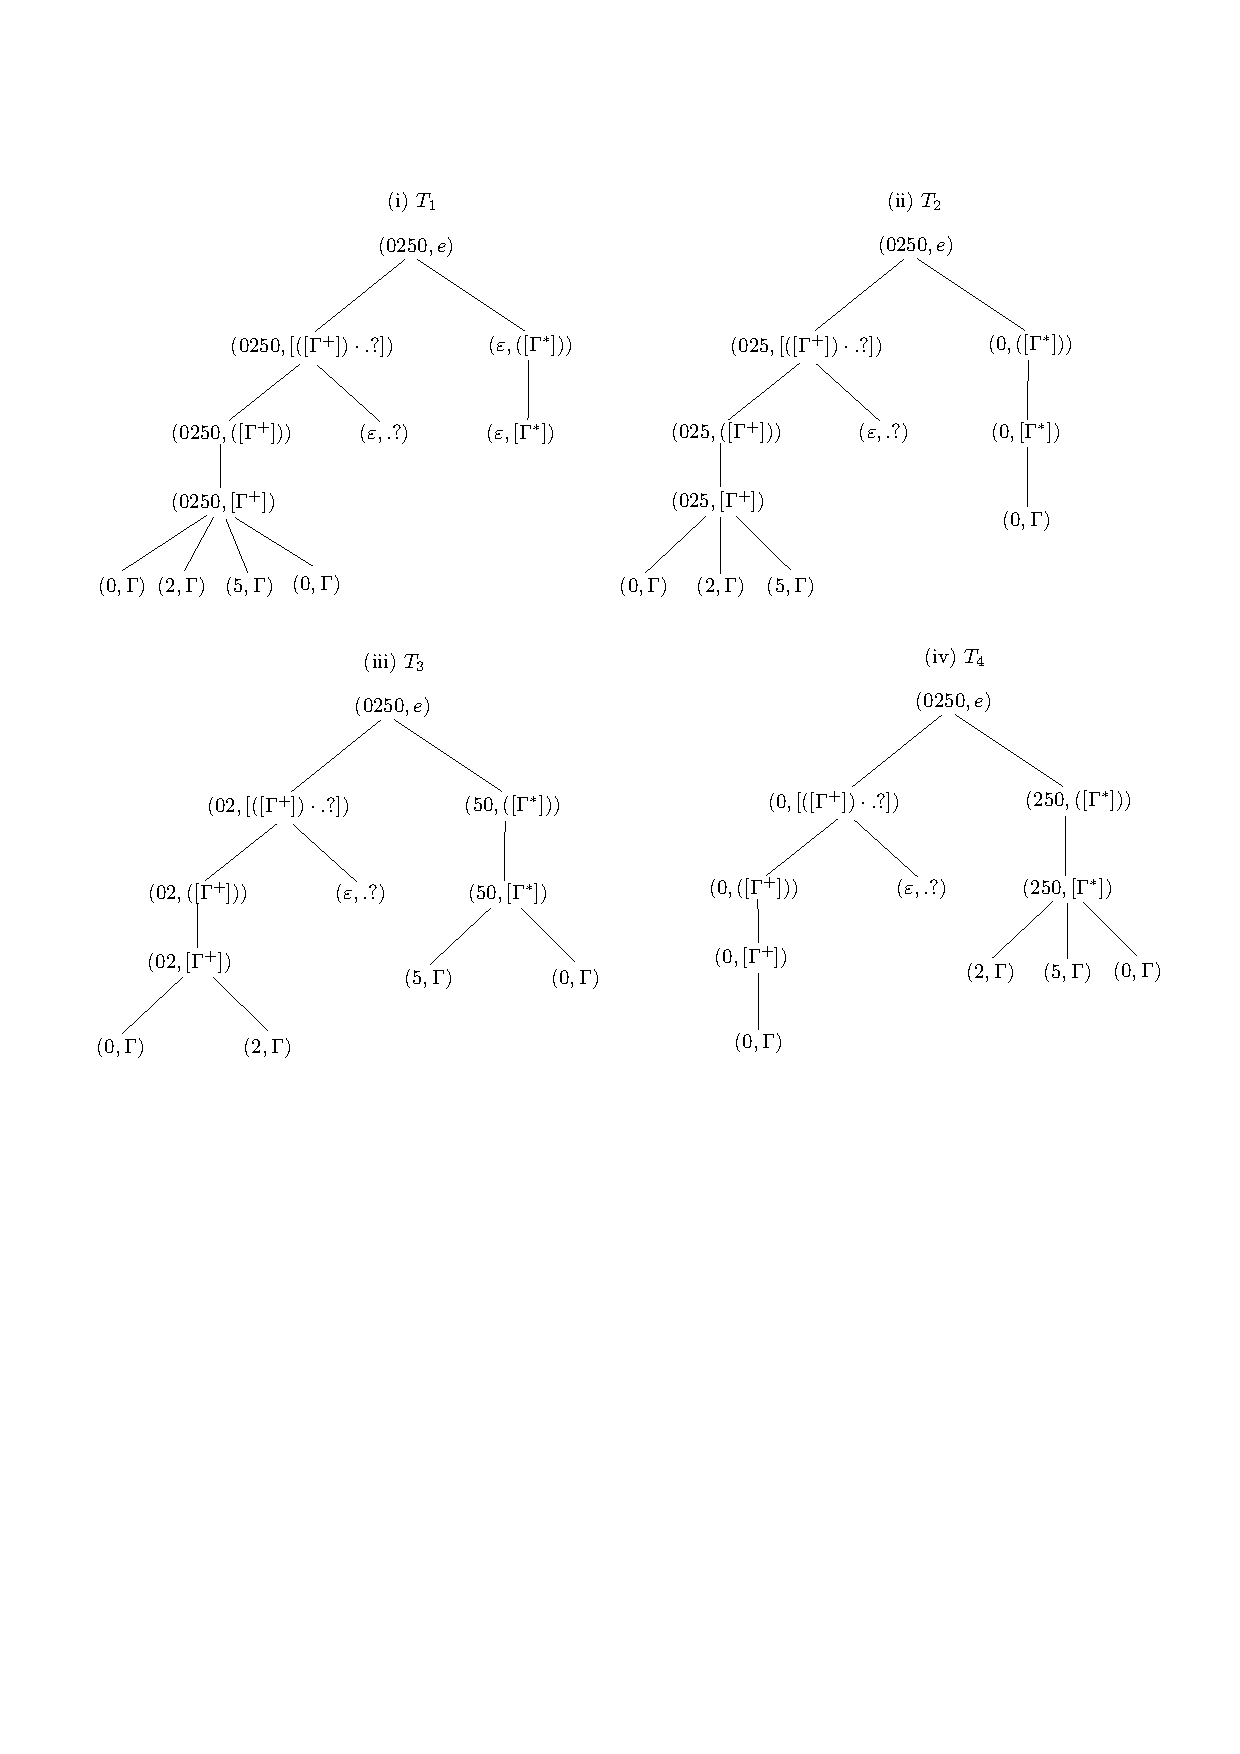
\includegraphics[width=1\textwidth]{regex-semantics-decimal.pdf}
\caption{Match trees of $e=[[([\Gamma^+])\concat .?] \concat ([\Gamma^*])]$ to $w= 0250$}
\label{fig-regex-semantics-decimal}
\end{figure}
%\Blindtext
 \end{example}



%%%%% the original example %%%%%%%%%%
%%%%% the original example %%%%%%%%%%
\hide{  
\begin{example}\label{exmp-regex-match-tree}
Let $e = ((b^\ast) \cdot ((b \cdot a^\ast) | \varepsilon)) \cdot a^\ast$ and $w= baa$. Then $\cM_{w}(e) = \{T_1,T_2,T_3\}$ as illustrated in Figure~\ref{fig-regex-semantics}: (i), (ii), (iii).  
\begin{figure}[ht]
\centering
%\rule{\linewidth}{0cm}
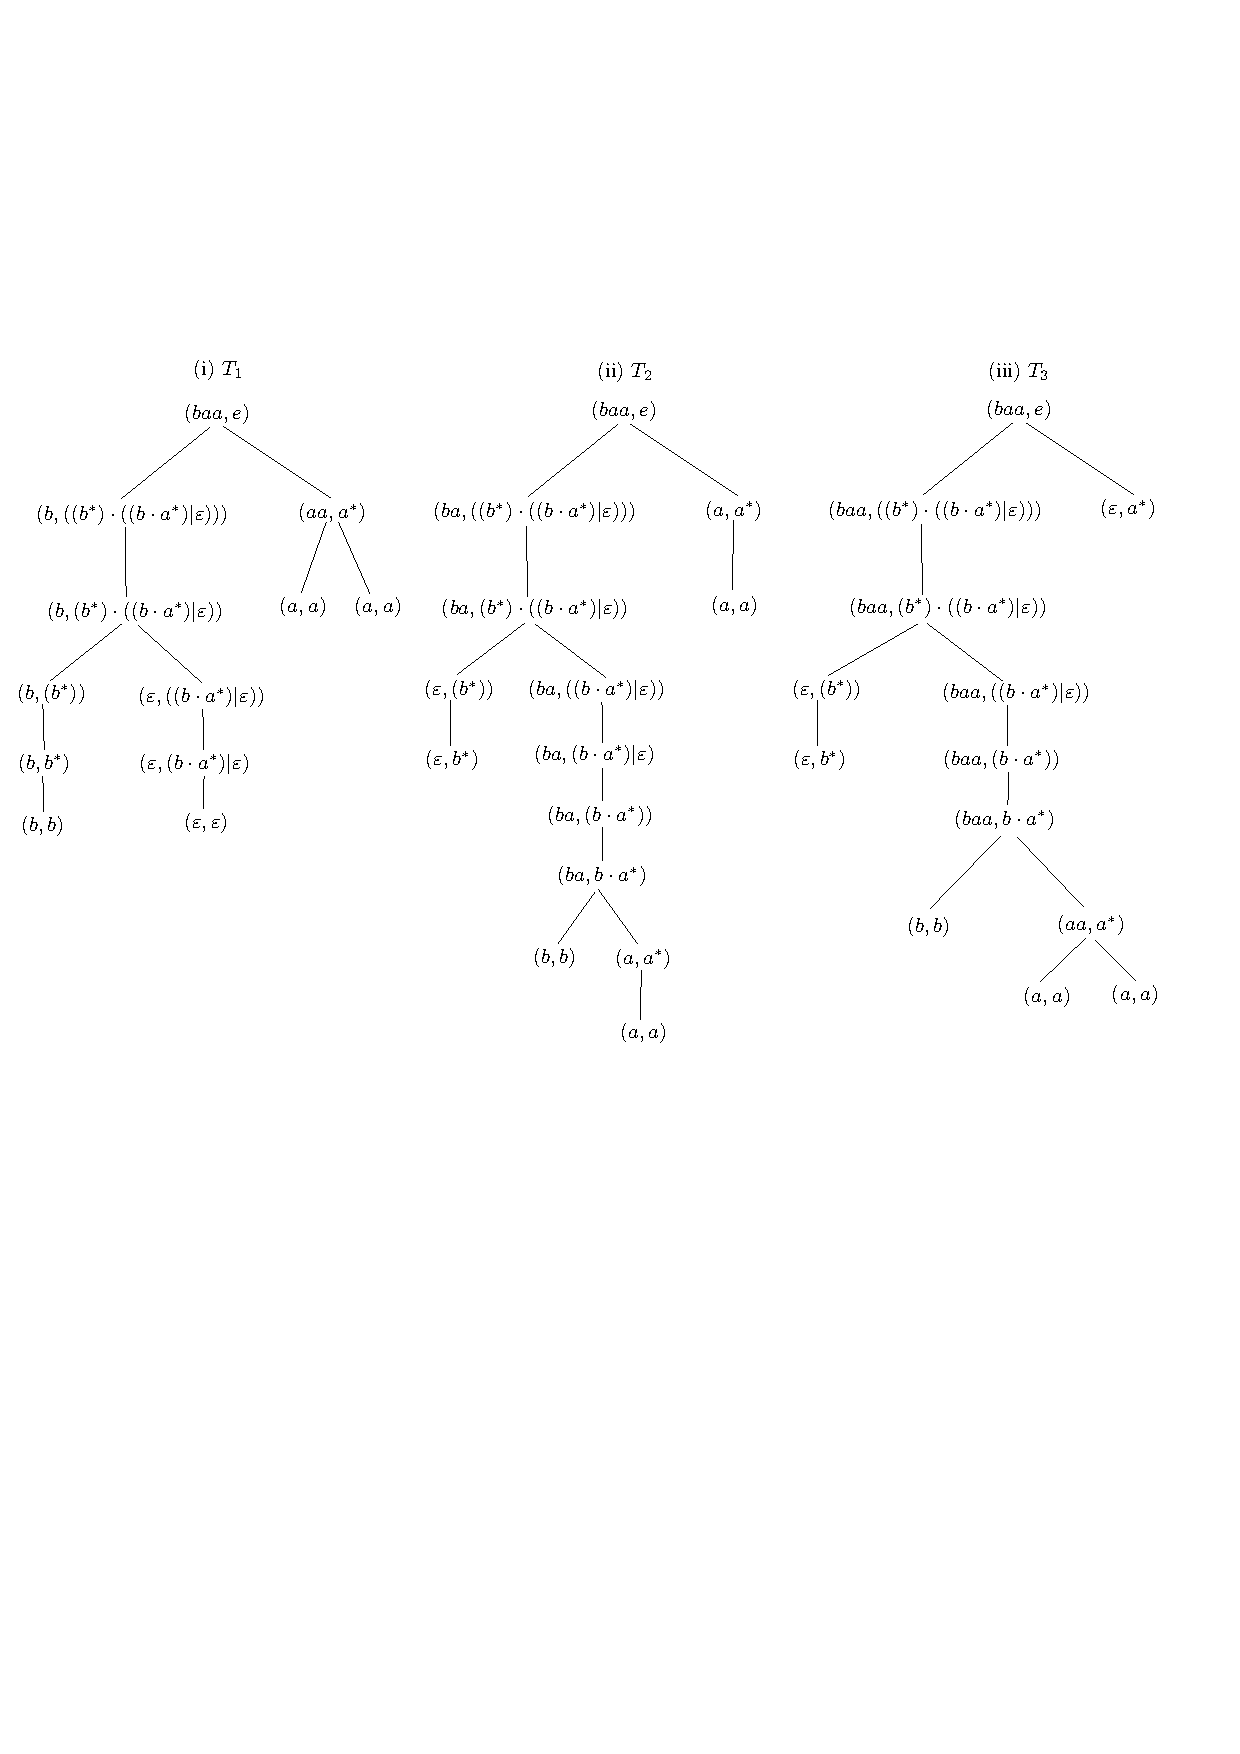
\includegraphics[width=1\textwidth]{regex-semantics.pdf}
\caption{Match trees of $e=((b^\ast) \cdot ((b \cdot a^\ast) | \varepsilon)) \cdot a^\ast$ to $w= baa$}
\label{fig-regex-semantics}
\end{figure}
%\Blindtext
 \end{example}
 }
 %%%%% the original example %%%%%%%%%%
%%%%% the original example %%%%%%%%%% 
  
  \begin{definition}[Semantics of $\regexp$]\label{def-regex-semantics}
  		
  	For a $\regexp$ $e$ and a string $w$, we recursively define a linear order on $\cM_{\pref(w)}(e)$, written $T
  	>_{w,e} T'$ for $T, T' \in \cM_{\pref(w)}(e)$, as follows:
  	\begin{itemize}
  		\item $e = \varepsilon$, $e = a$, or $e = \$ n$. There is only one match tree, thus the
  		order $>_{w, e}$ is empty.
 %
 		\item $e  = a?$. There are only two single-node match trees in $\cM_{\pref(w)}(e)$, namely, $(\varepsilon, e)$ and $(a, e)$. Then we have $(a, e) >_{w,e} (\varepsilon, e)$.
%		 		
  		\item $e = (e_1)$. Suppose that $C (T) = (w_1, e_1)$ and $C (T') = (w_2, e_1)$ for some $w_1, w_2 \in \pref(w)$.
  		Then $T >_{w,e} T'$ iff $T_{(w_1, e_1)} >_{w, e_1} T'_{(w_2, e_1)}$.
  		
  		\item $e = [e_1 + e_2]$.
  		\begin{itemize}
  			\item If $C (T) = (w_1, e_1)$ and $C (T') = (w_2, e_2)$ for some $w_1, w_2 \in \pref(w)$, then $T >_{w,e} T'$.
%  			
  			\item If $C (T) = (w_i, e_i)$ and $C (T') = (w'_i, e_i)$ for some $i \in \{ 1,
  			2 \}$ and $w_i, w'_i \in \pref(w)$, then $T >_{w,e} T'$ iff $T_{(w_i, e_i)} >_{w, e_i} T'_{(w'_i, e_i)}$.
  		\end{itemize}
  		\item $e = [e_1 \cdot e_2]$. Suppose $C (T) = (w_1, e_1) (w_2, e_2)$ and $C (T') =
  		(w_1', e_1) (w_2', e_2)$ (note that $w_1$ is a prefix of $w'_1$ or vice versa), then $T >_{w,e} T'$ when either $T_{(w_1, e_1)} >_{w, e_1}
  		T'_{(w_1', e_1)}$, or $w_1 = w_1'$ and $T_{(w_2, e_2)} >_{w_1^{-1}w, e_2} T'_{(w_2', e_2)}$. 
%  		
  		\item $e = [e_1^{\ast}]$. 
		\begin{itemize}
		\item If $T' $ is  a single node $(\varepsilon, e)$, but $T$ is not, then $T >_{w, e} T'$.
  		\item Otherwise, suppose $C(T) = (w_1, e_1) \ldots (w_k, e_1)$ and $C (T') =
  		(w_1', e_1)$ $\ldots$ $(w_l', e_1)$, we have $T >_{w,e} T'$ iff either when $C (T')$
  		is a proper prefix of $C (T)$, or for the first index $j$ such that $w_j
  		\neq w_j'$, we have $T_{(w_j, e_1)}$ $>_{(w_1\cdots w_{j-1})^{-1}w, e_1}$ $T'_{(w_j', e_1)}$.
		\end{itemize}
%
  		\item $e = [e_1^{\ast?}]$. 
		\begin{itemize}
		\item If $T$ is  a single node  $(\varepsilon, e)$, but $T'$ is not, then $T >_{w, e} T'$.
  		\item Otherwise, suppose $C(T) = (w_1, e_1) \ldots (w_k, e_1)$ and $C (T') =
  		(w_1', e_1)$ $\ldots$ $(w_l', e_1)$, we have $T >_{w,e} T'$ iff either when $C (T)$
  		is a proper prefix of $C (T')$, or for the first index $j$ such that $w_j
  		\neq w_j'$, we have $T_{(w_j, e_1)}$ $>_{(w_1\cdots w_{j-1})^{-1}w, e_1}$ $T'_{(w_j', e_1)}$.
		\end{itemize}
  	\end{itemize}
  	
  	For $e \in \regexp$ and $w \in \Lang(e)$, the \emph{accepting match} of $e$ to $w$, denoted by $M_e(w)$, is the supremum of $\cM_w(e)$. Moreover,  for $e \in \regexp$ and $w \in \Sigma^\ast$, if $w \in \Sigma^\ast \Lang(e)\Sigma^\ast$, then the (first) \emph{match} of $e$ in $w$ is defined as the supremum of $\cM_{\pref(w_1^{-1}w)}(e)$ such that $w_1$ is the shortest prefix of $w$ satisfying that $w_1^{-1}w \in \Lang(e)\Sigma^\ast$. If $w \not \in \Sigma^\ast \Lang(e)\Sigma^\ast$, the match of $e$ in $w$ is undefined.  
%  	
%  	For any subexpression $e'$ of $e$, suppose $(w_1, e') \ldots (w_m, e')$ are
%  	all the nodes labeled by $(w', e')$ with $w' \neq \varepsilon$, in the
%  	pre-order traversal of $M_e(w)$. Then the match result captured by $e'$, denoted
%  	by $M_{e', e} (w)$, is the sequence of substrings $w_1 \ldots w_m$.
  \end{definition}

\begin{example}\label{exmp-regex-semantics}
Let us continue Example~\ref{exmp-regex-match-tree}.  In Figure~\ref{fig-regex-semantics-decimal}, we have $(T_1)_{(0250, [\Gamma^+])} >_{(w, e)} (T_2)_{(025, [\Gamma^+])}$, since $(0, \Gamma)(2, \Gamma)(5,\Gamma)$ is a proper prefix of $(0, \Gamma)(2, \Gamma)(5,\Gamma)(0, \Gamma)$. From this, we deduce that $(T_1)_{(0250, ([\Gamma^+]))} >_{(w, e)} (T_2)_{(025, ([\Gamma^+]))}$. Therefore, $(T_1)_{(0250, [([\Gamma^+]) \concat .?])} >_{(w, e)} (T_2)_{(025,  [([\Gamma^+]) \concat .?])}$ and $T_1 >_{(w,e)} T_2$. Similarly, we have $T_2 >_{(w,e)} T_3$ and $T_3 >_{(w,e)} T_4$. Therefore, $T_1$ is the accepting match of $e$ to $w$, where the first and second capturing group of $e$ are matched to $0250$  and $\varepsilon$ respectively. 
%\Blindtext
 \end{example}
  
\begin{remark}
The semantics of $\regexp$ in Definition~\ref{def-regex-semantics} is essentially the semantics of regular expressions in Perl, PHP, and JavaScript etc. \cite{MasterREbook}. In comparison, POSIX regular expressions require the leftmost and longest match, which we leave as the future work. 
\end{remark}
  
  
% some examples
  
%  e = b(a*)a*
%  
%  e' = b(a*?)a*


%%%%%%%%%%%%%%%%%%%%%%%%%%%% 

%!TEX root = main.tex

\section{The string logic}\label{sec:logic}



%%%%%%%%%%%%%%%%%%%%%%%%%%%%%%%%%%%%%%%%


%\subsection{Prioritized Streaming String Transducer}
%Below, we introduce  a new class of prioritized transducer \cite{BM17} which combines the expressive power of streaming string transducer \cite{AC10,AD11}.
%
%\begin{definition}[Prioritized Streaming String Transducer]
%	A \emph{prioritized streaming string transducer} (PSST) is a tuple $\psst = (Q, \Sigma, X, E, \delta, q_0, F)$, where $Q$ a
%	finite set of states, $\Sigma$ is the input and output alphabet, and $X$ a finite set of variables. $E$ is a partial function from $Q \times \Sigma \times
%	Q$ to $X \rightarrow (X \cup \Sigma)^{\ast}$, i.e. the set of assignment,
%	$\delta \in Q \times \Sigma \rightarrow \overline{Q}$ and $F$ is a partial function
%	from $Q$ to $(X \cup \Sigma)^{\ast}$.
%\end{definition}
%
%A run of $\psst$ is the sequence $q_0 \sigma_1 s_1 q_1 \ldots \sigma_m s_m q_m$, where $F (q_m)$ is defined and for each $i \in [m], q_i \in \delta (q_{i-1}, \sigma_i)$ and $s_i = E (q_{i - 1}, \sigma_i, q_i)$. For any two runs on $w = \sigma_1 \ldots \sigma_m$, denoted by $p = q_0 \sigma_1 s_1 \ldots \sigma_m s_m q_m$ and $p' = q_0 \sigma_1
%s_1' \ldots \sigma_m s_m' q_m'$, we say that $p$ is of a higher priority over
%$p'$ if $p \neq p'$ and, for the smallest index $j$ with $q_j \neq q_j'$,
%$\delta (q_{j - 1}, \sigma_j) = \ldots q_j \ldots q_j' \ldots$
%
%The accepting run of $\psst$ on input $w$ is the run of the highest priority. The output of $T$ on w, denoted by $T(w)$, is defined as $\pi_m(F(q_m))$, where $\pi_0(x) = \varepsilon$ for each $x \in X$, and $\pi_{i}(x) = \pi_{i-1}(s_{i}(x))$ for $1 \le i \le m$ and $x \in X$. Note that here we abuse the notation  $\pi_m(F(q_m))$ and $\pi_{i-1}(s_{i}(x))$ by taking a function $\pi$ from $X$ to $\Sigma^*$ as a function from $(X \cup \Sigma)^*$ to $\Sigma^*$, which maps each $\sigma \in \Sigma$ to $\sigma$ and each $x \in X$ to $\pi(x)$.  
%
%%  $\tmop{Out} (r) =
%%  s_{\varepsilon} \circ s_1 \circ s_2 \ldots s_n \circ F (q_n)$ where
%%  $s_{\varepsilon}$ is the empty substitution which maps all variables to
%%  $\varepsilon$.
%
%\begin{definition}[pre-image]
%	For a string relation $R \subseteq \Sigma^* \times \Sigma^*$ and $L \subseteq \Sigma^*$, we define the \emph{pre-image} of $L$ under $R$ as $R^{-1}(L):=\{w \in \Sigma^* \mid \exists w'.\ w' \in L \mbox{ and } (w, w') \in R\}$. 
%\end{definition}
%
%\begin{theorem}[pre-image of \PSST{}]
%	\label{theorem:psst_preimage}
%	Given a \PSST{} $\psst = (Q_T, \Sigma$, $X, E, \delta_T, q_{0, T}, F_T)$ and \FA{} $A
%	= (Q_A, \Sigma, \delta_A, q_{0, A}, F_A)$, we can compute an \FA{} $B = (Q_B,
%	\Sigma, \delta_B, q_{0, B}, F_B)$ in exponential time  such that $\Lang(B) = \cR^{-1}_T(\Lang(\Aut))$.
%\end{theorem}
%
%\begin{proof}
%	Intuitively, $B$ simulates the run of $\psst$ on $w$, and, for each $x \in X$, records the set of state pairs $(p, q) \in Q_A \times Q_A$ such that starting from $p$, $A$ can reach $q$ after reading the string stored in $x$. Moreover, $B$ also records all the states accessible from a run with higher priority to ensure the current run is the accepting one of $\psst$.
%	
%	Formally, $Q_B = Q_T \times (\cP(Q_A \times Q_A ))^{X} \times \cP(Q_T)  $, $q_{0, B} = (q_{0, T}, \rho_{\varepsilon}, \emptyset)$ where $\rho_{\varepsilon} (x) = \{(q, q) \mid q \in Q\}$ for each $x \in X$, and $\delta_{B}$ comprises the tuples $((q, \rho, S), a, (q_i, \rho', S'))$ such that there exists $s \in \left((X \cup \Sigma\right)^*)^X$ satisfying
%	\begin{itemize}
%		\item $\delta_T (q, a) = (q_1 \ldots q_i \ldots q_m)$, 
%		\item $s = E(q,a,q_i)$.
%		\item $S' = \delta_T^{\ast} (S, a) \cup \{ q_1, \ldots, q_{i - 1} \}$, where $\delta_T^{\ast}(S,a) = \{q' \mid \exists q \in S, q' \in \delta_T(q,a)\}$.
%		\item and $\rho'$ is obtained from $\rho$ and $s$ as follows: for each $x \in X$, if $s(x) = \varepsilon$, then $\rho'(x) = \{(p, p) \mid p \in Q_A\}$, otherwise, let $s(x) = b_1 \cdots b_\ell$ with $b_i \in \Sigma \cup X$ for each $i \in [\ell]$, then $\rho'(x) = \theta_1 \circ \cdots \circ \theta_\ell$, where $\theta_i = \delta^{(b_i)}_A$ if $b_i \in \Sigma$, and $\theta_i = \rho(b_i)$ otherwise.
%		%
%		%$\rho'(x) = \theta_\ell$ such that $\theta_0 = \{(p,p) \mid p \in Q_A\}$, and for each $i \in [\ell]$, if $b_i \in \Sigma$, then $\theta_i = \{(p, p') \mid (p, p'') \in \theta_{i-1}, (p'', b_i, p') \in \delta_A \mbox{ for some } p''\}$, otherwise, $\theta_i = \theta_{i-1} \cdot \rho(x)$. 
%	\end{itemize}
%	
%	Moreover, $F_B$ is the set of states $(q, \rho, S) \in Q_B$ such that
%	\begin{enumerate}
%		\item $F_T (q)$ is defined,
%		\item For any $q' \in S$, $F_T (q')$ is not defined
%		
%		\item if $F_T(q) = \varepsilon$, then $q_{0, A}  \in F_A$, otherwise, 
%		let $F_T(q) = b_1 \cdots b_\ell$ with $b_i \in \Sigma \cup X$ for each $i \in [\ell]$, then $(\theta_1 \circ \cdots \circ \theta_\ell) \cap (\{q_{0,A}\} \times F_A) \neq \emptyset$, where for each $i \in [\ell]$, if $b_i \in \Sigma$, then $\theta_i = \delta^{(b_i)}_A$, otherwise, $\theta_i = \rho(b_i)$.
%	\end{enumerate}
%\end{proof}
%
%Note that the above construction  does not utilize the so-called \tmtextit{copyless} property \cite{AC10,AD11},
%thus it works for general, or \tmtextit{copyful} \PSST{} \cite{FR17}.

% Note that in the definition of \NSST, there is no \emph{copyless} restriction.



%%%%%%%%%%%%%%%%%%%%%%%%%%%%%%%%%%%%%%%%%%%%%%%%%%%%%


%We will use $\$ 1, \$2, \cdots$ to denote the references to capturing groups in regular expressions.

%We define the set of reference expressions as follows: 

%We consider the symbolic execution of the string-manipulating programs.

%\begin{definition}[The constraint language $\strline$] 
We define the string-manipulating language $\strline$ %considered in this paper 
as follows. 
%The $\strline$ language is defined by
\[
\begin{array}{l}
S \eqdef  z:= x \concat y \mid y := \extract_{i, e}(x) \mid  
%& &  
%y := \reverse(x) 
y := \replaceall_{\pat, \rep}(x)   \mid 
%y := \Transducer(x)\  \mid\\
 \ASSERT{x \in e} \mid S; S\
\label{eq:SL}
%a ::= f(x_1,\ldots,x_n), \qquad b ::= g(x_1,\ldots,x_n)
\end{array}
\]
%\tl{to avoid confusion, write  $\ASSERT{x \in A}$?} 
where 
\begin{itemize}
	\item $\concat$ is the string concatenation operation which concatenates two strings,
%
\item for the $\extract$ function, $i \in \Nat$, $e \in \cgexp$,
%
	\item  for the $\replaceall$ operation, $\pat\in \cgexp$, $\rep \in \refexp$, %$\replaceall$ is the replace-all function to be defined shortly,
%	\item $\reverse$ is the string function which reverses a string; 
%	\item $\Transducer$ is a \PSST,
%
	\item for assertions, $e \in \regexp$.
\end{itemize} 
%and $R$ is a recognisable relation represented by a collection of tuples of \FA{}s.
%\end{definition}
%
%\zhilei{Should we add NSST constraints? Basically NSST can express more than PSST.}
%\tl{maybe just use NSST to replace PSST?}
%
%\zhilei{PSST is needed for decision procedure. NSST can be decided too, but the algorithm is very similar, so maybe too tedious to add both }

%It is evident that the $\reverse$ function is subsumed by \PSST{}s.

%
%\begin{remark}
%	Zhilin mentioned that we might introduce a function which takes a string and a pattern with capturing groups, and does sort of pattern matching to extra substrings. This function can be captured by the transducer $T$. We will formalise this later.
%\end{remark}

The $\extract$ function is used to model the regular-expression match function in programming languages.
%, e.g. $\sf str.match(regexp)$ function in Javascript. 
Specifically, the $\extract_{i, e}(x)$ function extracts the match of the $i$-th capturing group in the accepting match of $e$ to $x$ for $x \in \Lang(e)$ (otherwise, the return value of the function is undefined). Note that $\extract_{i, e}(x)$ returns $x$ if $i=0$. For instance, assuming $e = [[([\Gamma^+])\concat .?] \concat ([\Gamma^*])]$,   $\extract_{1, e}(0250)=0250$ and $\extract_{2, e}(0250)=\varepsilon$, as shown in Example~\ref{exmp-regex-semantics}. 

\begin{remark}
The match function in programming languages, e.g. $\sf str.match(reg)$ function in JavaScript, finds the first match of $\sf reg$ in $\sf str$. We can use $\extract$ to express the first match of $\sf reg$ in $\sf str$ by adding $[\Sigma^{*?}]$ and $[\Sigma^*]$ before and after $\sf reg$ respectively. More generally, the value of the $i$-th capturing group in the first match of a $\regexp$ $\sf reg$ in $\sf str$ can be specified as $\extract_{i+1, {\sf reg'}}({\sf str})$, where ${\sf reg'} = [[[\Sigma^{*?}] \concat ({\sf reg})] \concat [\Sigma^*]]$.
\end{remark}

The $\replaceall_{\pat, \rep}(x)$ function is parameterized by the  %\emph{subject} string, the second parameter is a 
\emph{pattern} $\pat \in \cgexp$ and the \emph{replacement} string $\rep \in \refexp$. For a given input string $x$, the function identifies all the %the first, second, $\dots$, 
matches of $\pat$ in $x$ and replace them with the corresponding strings specified by the replacement string. (In the replacement string,  references may be used which refer to %are replaced by 
the corresponding matches of the capturing groups.)  For instance, let $\pat = [[([\Gamma^+])\concat .?] \concat ([\Gamma^*])]$ and $\rep = \$1$. We have $\replaceall_{\pat, \rep}(2.5,3.4) = 2,3$. 

Without loss of generality, we assume that all the $\strline$ programs are in single static assignment (SSA) form, that is, each variable $x$ is assigned at most once. Moreover, if it is assigned, all its occurrences on the right hand sides of the assignment statements or in assertions are after the assignment statement of $x$.
%
For an $\strline$ program $S$, a variable $x$ occurring in $S$ is said to be an \emph{input} variable if $x$ does not occur on the left hand sides of assignment statements. The \emph{path feasibility} problem of an $\strline$ program is to decide whether there are valuations of the input variables such that the program can execute to the end.


%
%For the semantics of $\replaceall$ function, in particular when the pattern is a regular expression, we adopt the \emph{leftmost and longest} matching. 




%For instance, $\replaceall(aababaab, (ab)^+, c) =ac\cdot \replaceall(aab, (ab)^+, c)= acac$, since the leftmost and longest matching of $(ab)^+$ in $aababaab$ is $abab$. Here we require that the language defined by the pattern parameter does \emph{not} contain the empty string, in order to avoid the troublesome definition of the semantics of the matching of the empty string. We refer the reader to \cite{CCHLW18} for the formal semantics of the $\replaceall$ function. To be consistent with the notation in this paper, for each regular expression $e$, we define
%the string function $\replaceall_e: \ialphabet^* \times \ialphabet^* \rightarrow \ialphabet^*$ such that for $u, v \in \ialphabet^*$, $\replaceall_e(u, v) = \replaceall(u, e, v)$, and we write $\replaceall(x, e, y)$ as $\replaceall_e(x,y)$.

It turns out that the path feasibility problem is undecidable, attributed to the the back references in assertion statements. 

\begin{proposition}\label{prop-und}
The path feasibility problem of $\strline$ is undecidable.
\end{proposition}

We shall show that the path feasibility problem is decidable, if the uses of back references in assertion statements are forbidden, which turns out to be the situation in practice.\footnote{A partial evidence is that the occurrences of regular expressions with back references occupy only less than $1\%$ in the NPM package, according to the statistics collected in \cite{LMK19}.} In the sequel, we will use $\strline_{\sf reg}$ to denote the collection of $\strline$ programs which are free of %where no 
back references in assertion statements. %We state 
The main result of this paper is as follows.

\begin{theorem}\label{thm-main}
The path feasibility of $\strline_{\sf reg}$ is decidable in XXX. \zhilin{complexity should be added}
\end{theorem}
The decision procedure for $\strline_{\sf reg}$ utilizes a new model called prioritized streaming string transducers, which will be defined in the next section.


%%%%%%%%%%%%%%%%%%%%%%%%%%%%

%!TEX root = main.tex
 
{\PSST}s can be seen as an extension of finite-state automata with transition priorities and string variables. We first recall the definition of classic finite-state automata.

\begin{definition}[Finite-state Automata] \label{def:nfa}
	A \emph{(nondeterministic) finite-state automaton}
	(\FA{}) over a finite alphabet $\ialphabet$ is a tuple $\Aut =
	(\ialphabet, \controls, q_0, \finals, \transrel)$ where 
	$\controls$ is a finite set of 
	states, $q_0\in \controls$ is
	the initial state, $\finals\subseteq \controls$ is a set of final states, and 
	$\transrel\subseteq \controls \times 
	\ialphabet^\varepsilon \times  \controls$ is the
	transition relation. 
\end{definition}

For an input string $w$, a \emph{run} of $\Aut$ on $w$
%(with $a_0 = \EndLeft$ and $a_{n+1} = \EndRight$)
is a sequence $q_0 a_1 q_1 \ldots a_n q_n$ such that $w = a_1 \cdots a_n$ and $(q_{j-1}, a_{j}, q_{j}) \in
\transrel$ for every $j \in [n]$.
%
The run is said to be \defn{accepting} if $q_n \in \finals$.
A string $w$ is \defn{accepted} by $\Aut$ if there is an accepting run of
$\Aut$ on $w$. 
%In particular, the empty string $\varepsilon$ is accepted by $\Aut$ if $q_0 \in F$. 
The set of strings accepted by $\Aut$, i.e., the language \defn{recognized} by $\Aut$, is denoted by $\Lang(\Aut)$.
%Since we deal with computational complexity in the sequel, we define
The \defn{size} $|\Aut|$ of $\Aut$ is the cardinality of $\transrel$, the set of transitions.


%%%%%%%%%%%%%%%%%%%%%%%%%%%%%%%%%%%%%%%%%%%%%%%%
%%%%%%%%%%%%%%%%%%%%%%%%%%%%%%%%%%%%%%%%%%%%%%%%
\OMIT{
\begin{definition}[Prioritized Finite-state Automata]\label{def-pfa}
	A \emph{prioritized finite-state automaton} (PFA) over a finite alphabet $\Sigma$ is a tuple $\pnfa=(Q, \Sigma, \delta, \tau, q_0, F)$ where $\delta \in Q
	\times \Sigma \rightarrow \overline{Q}$ and $\tau \in Q \rightarrow \overline{Q} \times \overline{Q}$ such that for every $q \in Q$, if $\tau(q) = (P_1; P_2)$, then $P_1 \cap P_2 = \emptyset$. 
	The definition of $Q$, $q_0$ and $F$ is the same as FA.
\end{definition}
For $\tau(q)=(P_1; P_2)$, we will use $\pi_1(\tau(q))$ and $\pi_2(\tau(q))$ to denote $P_1$ and $P_2$ respectively.  With slight abuse of notation, we write $q\in (P_1; P_2)$ for $q\in P_1\cup P_2$. Intuitively, $\tau(q)=(P_1; P_2)$ specifies the $\varepsilon$-transitions at $q$, with the intuition that the $\varepsilon$-transitions to the states in $P_1$ (resp. $P_2$) have higher (resp. lower) priorities than the non-$\varepsilon$-transitions out of $q$.

A \emph{run} of $\pnfa$ on a string $w$ is a sequence $q_0 a'_1 q_1 \ldots a'_m q_m$ such that 
\begin{itemize}
	%\item $q_m \in F$,
	\item for any $i \in [m]$, either $a'_i \in \Sigma$ and $q_i \in \delta (q_{i - 1}, a'_i)$, or $a'_i = \varepsilon$ and $q_i \in \tau(q_{i-1})$, %\pi_1(\tau(q_{i-1}))\cup \pi_2(\tau(q_{i-1}))$,
	\item $w = a'_1 \cdots a'_m$,
	%
	\item for every subsequence $q_i a'_{i+1} q_{i+1} \ldots a'_{j} q_j$ such that  $i < j$ and $a'_{i+1} = \cdots = a'_j = \varepsilon$, it holds that for every $k, l: i \le k < l < j$, $(q_k, q_{k+1}) \neq (q_l, q_{l+1})$.
	%each state $q \in Q$ occurs \emph{at most twice} in the subsequence. 
	(Intuitively, each transition occurs at most once in a sequence of $\varepsilon$-transitions.) 
	%
	%\item moreover, for every suffix $q_i a'_{i+1} q_{i+1} \ldots a'_{m} q_m$ such that $i < m$ and $a'_{i+1} = \cdots = a'_m = \varepsilon$, it holds that $q_i, \dots, q_m$ are mutually distinct.  (Intuitively, each state occurs at most once in a suffix of $\varepsilon$-transitions.) 
\end{itemize}

Note that it is possible that $\delta(q, a) = ()$, that is, there is no $a$-transition out of $q$. 
It is easy to observe that, given a string $w$, the length of a run of $\pnfa$ on $w$ is $O(|w||\cA|)$. 
For any two runs $R = q_0 a_1 q_1 \ldots a_m q_m$ and $R' =  q_0 a'_1 q_1' \ldots a'_n q'_n$ such that $a_1 \ldots a_m = a'_1 \ldots a'_n$, we say that $R$ is of a higher priority over $R'$ if 
\begin{itemize}
	\item either $R'$ is a prefix of $R$ (in this case, the transitions of $R$ after $R'$ are all $\varepsilon$-transitions), 
	%
	\item or there is an index $j$ satisfying one of the following constraints:
	\begin{itemize}
		\item $q_0 a_1 q_1 \ldots q_{j-1} a_j = q_0 a'_1 q'_1 \ldots q'_{j-1} a'_j$, $q_j \neq q'_j$, $a_j \in \Sigma$, and $\delta (q_{j - 1}, a_j) =(\ldots, q_j, \ldots, q_j', \ldots)$,
		%
		\item $q_0 a_1 q_1 \ldots q_{j-1} a_j = q_0 a'_1 q'_1 \ldots q'_{j-1} a'_j$, $q_j \neq q'_j$, $a_j  = \varepsilon$,  and one of the following conditions holds: (i) $\pi_1(\tau(q_{j - 1})) = (\ldots, q_j, \ldots, q_j', \ldots)$, (ii) $\pi_2(\tau(q_{j - 1})) = (\ldots, q_j, \ldots, q_j', \ldots)$, or (iii) $q_j \in \pi_1(\tau(q_{j - 1}))$ and $q'_j \in \pi_2(\tau(q_{j-1}))$, 
		%
		\item $q_0 a_1 q_1 \ldots q_{j-1}  = q_0 a'_1 q'_1 \ldots q'_{j-1} $, $a_j  = \varepsilon$, $a'_j  \in \Sigma$, $q_j \in \pi_1(\tau(q_{j - 1}))$, and $q'_j \in \delta(q_{j-1}, a'_j)$, 
		%
		\item $q_0 a_1 q_1 \ldots q_{j-1}  = q_0 a'_1 q'_1 \ldots q'_{j-1} $, $a_j  \in \Sigma$, $a'_j  = \varepsilon$, $q_j \in \delta(q_{j - 1}, a_j)$, and $q'_j \in \pi_2(\tau(q_{j-1}))$.
	\end{itemize}
\end{itemize}
%From the definition of ``higher priorities" above, we observe that if there is a  run of $\pnfa$ on a string $w$, then there is a unique run of $\pnfa$ on $w$ with the highest priority. 
An \emph{accepting} run of $\pnfa$ on $w$ is a run $R = q_0 a_1 q_1 \ldots a_m q_m$ of $\pnfa$ on $w$ satisfying that 1) $q_m \in F$, 2) $R$ is of the \emph{highest} priority among those runs satisfying $q_m \in F$. 
%(Note that a run $q_0 a_1 q_1 \ldots a_m q_m$ of $\pnfa$ on $w$ with the highest priority may not satisfy $q_m \in F$.) 

The language of $\pnfa$, denoted by $\Lang(\pnfa)$, is the set of strings on which $\pnfa$ has an accepting run.
%
Note that the priorities in PFAs have no impact on whether a string is accepted; rather they affect the way that the string is accepted. As a result, PFAs still define the class of regular languages. 
}
%%%%%%%%%%%%%%%%%%%%%%%%%%%%%%%%%%%%%%%%%%%%%%%%
%%%%%%%%%%%%%%%%%%%%%%%%%%%%%%%%%%%%%%%%%%%%%%%%


%In this section, we introduce prioritized streaming string transducers (PSST), 
%a new class of transducers that combine prioritized finite-state automata \cite{BM17} 
%and streaming string transducers \cite{AC10,AD11}.
%We shall utilize PSSTs to model greedy/lazy semantics of Kleene star/plus as well as the behavior of the $\extract$ and $\replaceall$ functions.



%%%%%%%%% The old example for PFA %%%%%%%%%
%\hide{
%\begin{example}\label{exmp-pfa}
%The PFAs corresponding to $a^\ast$ and $a^{\ast?}$ respectively are illustrated in Figure~\ref{fig-pfa}(i) and (ii), where the dashed line represents $\pi_2(\tau(q_0))$ (of lower priority than the $a$-transition), the thicker solid line represents $\pi_1(\tau(q_0))$ (of higher priority than the $a$-transition), and the doubly circled state $q_1$ is a final state.
%
%\begin{figure}[ht]
%\centering
%%\rule{\linewidth}{0cm}
%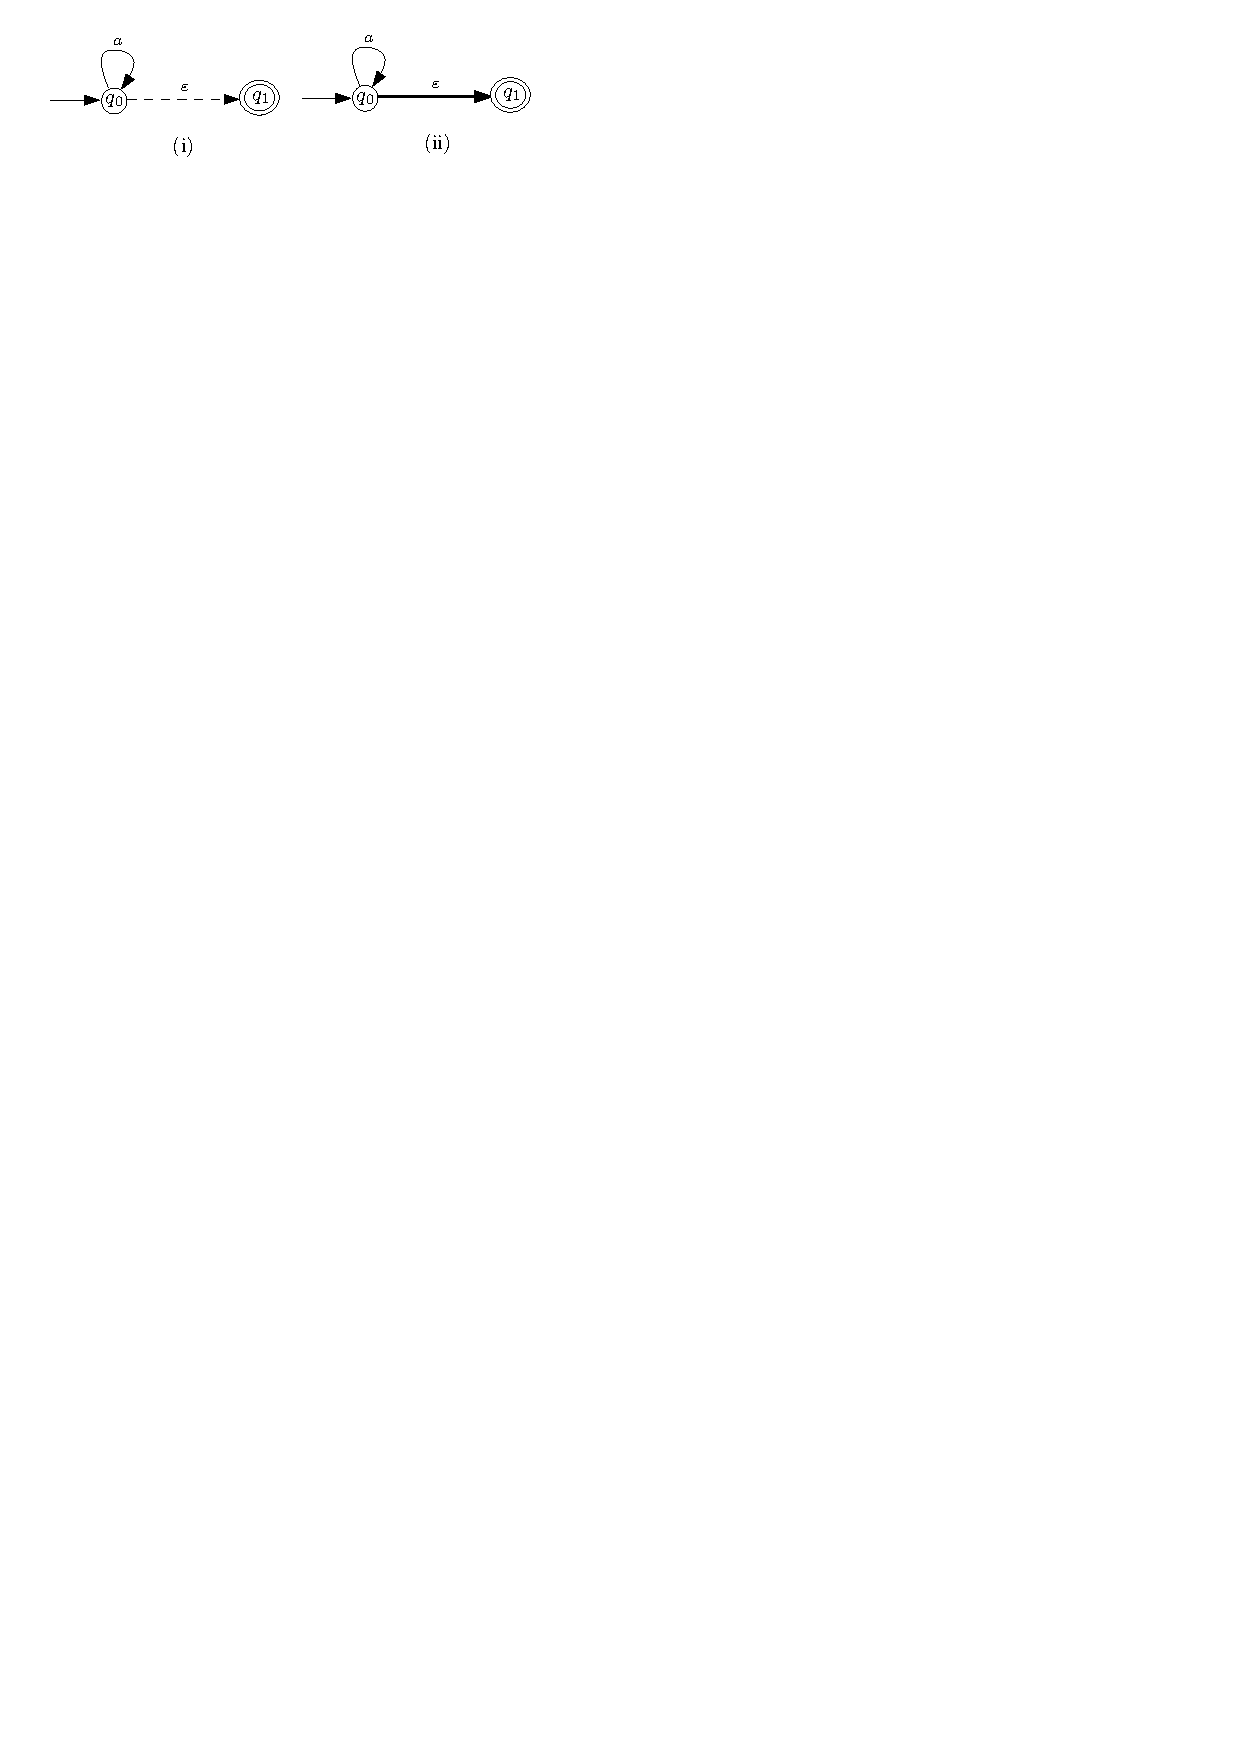
\includegraphics[width=0.6\textwidth]{pfa.pdf}
%\caption{The PFAs for $a^\ast$ and $a^{\ast?}$}
%\label{fig-pfa}
%\end{figure}
%\end{example}
%}
%%%%%%%%% The old example %%%%%%%%%

%\begin{remark}
%Remark that PFAs in Definition~\ref{def-pfa} are different from pNFAs in \cite{BM17} in the sense that the state set in a pNFA is partitioned into two disjoint subsets and the non-$\varepsilon$-transitions are deterministic, while this is not the case in PFAs. Therefore, PFAs are slightly more flexible than pNFAs in \cite{BM17}. We choose this definition of PFAs as a more natural extension of FAs. 
%\end{remark}

%The priorities of PFAs are used to model the greedy and non-greedy semantics of $\regexp$. %, as we shall see in Section~\ref{construction:pnfa}.

%%%%%%%%%%%%%%%%%%%%%%%%%%%%%%%%%%%%%%%%%%%%%%%%%%%%%%%%%%%%%%%%%%%%%%%%%%%%%%%%%%%%%%%%%%%%%%%%%%
%PSST
%%%%%%%%%%%%%%%%%%%%%%%%%%%%%%%%%%%%%%%%%%%%%%%%%%%%%%%%%%%%%%%%%%%%%%%%%%%%%%%%%%%%%%%%%%%%%%%%%%%%%%%


%a new class of transducers that combine prioritized finite-state automata \cite{BM17} %which combines the expressive power of 
%and streaming string transducers \cite{AC10,AD11}.

For a finite set $Q$, let $\overline{Q} = \bigcup_{n\in \Nat}\{ (q_1, \ldots, q_n) \mid \forall i \in [n], q_i \in Q \wedge \forall i,j \in[n], i \neq j \rightarrow q_i \neq q_j \}$. Intuitively, $\overline{Q}$ is the set of sequences of non-repetitive elements from $Q$. In particular, the empty sequence $() \in \overline{Q}$. Note that the length of each sequence from $\overline{Q}$ is bounded by  $| Q |$. For a sequence $P = (q_1, \ldots, q_n) \in \overline{Q}$ and  $q \in Q$, we write $q \in P$ if  $q = q_i$ for some $i \in [n]$. Moreover, for $P_1 = (q_1, \ldots, q_m) \in \overline{Q}$ and $P_2 = (q'_1, \ldots, q'_n) \in \overline{Q}$, we say $P_1 \cap P_2 = \emptyset$ if $\{q_1, \ldots, q_m\} \cap \{q'_1, \ldots, q'_n\} = \emptyset$.
    


%%%%%%%%%%%%%%%%%%%%%%%%%%%%%%%%%%%%%%%%%%%%
%%%%%%%%%%%%%%%%%%%%%%%%%%%%%%%%%%%%%%%%%%%%
%\OMIT{
%\begin{definition}[Prioritized Streaming String Transducers]
%A \emph{prioritized streaming string transducer} (PSST) is a tuple $\psst = (Q, \Sigma, X, \delta, \tau, E, q_0, F)$, where $Q$ is a
%finite set of states, $\Sigma$ is the input and output alphabet such that $\nullchar \not \in \Sigma$, $X$ is a finite set of variables, $\delta \in Q \times \Sigma \rightarrow \overline{Q}$, $\tau \in Q \rightarrow \overline{Q} \times \overline{Q}$, $E$ is a partial function from $Q \times \Sigma^\varepsilon \times
%  Q$ to $X \rightarrow \{\nullchar\} \cup (X \cup \Sigma)^{\ast}$, i.e. the set of assignments,
%   $q_0 \in Q$ is the initial state, and $F$ is a partial function
%  from $Q$ to $(X \cup \Sigma)^{\ast}$.
%\end{definition}
%}
%%%%%%%%%%%%%%%%%%%%%%%%%%%%%%%%%%%%%%%%%%%%
%%%%%%%%%%%%%%%%%%%%%%%%%%%%%%%%%%%%%%%%%%%%


\begin{definition}[Prioritized Streaming String Transducers]
A \emph{prioritized streaming string transducer} (\PSST) is a tuple $\psst = (Q, \Sigma, X, \delta, \tau, E, q_0, F)$, where 
\begin{itemize}
\item $Q$ is a finite set of states, 
\item $\Sigma$ is the input and output alphabet, 
\item $X$ is a finite set of string variables, 
\item $\delta \in Q \times \Sigma \rightarrow \overline{Q}$ defines the non-$\varepsilon$ transitions as well as their priorities (from highest to lowest),
% 
\item $\tau \in Q \rightarrow \overline{Q} \times \overline{Q}$ such that for every $q \in Q$, if $\tau(q) = (P_1; P_2)$, then $P_1 \cap P_2 = \emptyset$, (Intuitively, $\tau(q)=(P_1; P_2)$ specifies the $\varepsilon$-transitions at $q$, with the intuition that the $\varepsilon$-transitions to the states in $P_1$ (resp. $P_2$) have higher (resp. lower) priorities than the non-$\varepsilon$-transitions out of $q$.)
\item $E$ associates with each transition a string-variable assignment function, i.e., $E$ is partial function from $Q \times \Sigma^\varepsilon \times
  Q$ to $X \rightarrow (X \cup \Sigma)^{\ast}$ such that its domain is the set of tuples $(q, a, q')$ satisfying that either $a \in \Sigma$ and $q' \in \delta(q, a)$ or $a = \varepsilon$ and $q' \in \tau(q)$,
\item  $q_0 \in Q$ is the initial state, and
\item  $F$ is the output function, which is a partial function from $Q$ to $(X \cup \Sigma)^{\ast}$.
\end{itemize}
\end{definition}
%
For $\tau(q)=(P_1; P_2)$, we will use $\pi_1(\tau(q))$ and $\pi_2(\tau(q))$ to denote $P_1$ and $P_2$ respectively.  
%With slight abuse of notation, we write $q\in (P_1; P_2)$ for $q\in P_1\cup P_2$. 
%Intuitively, $\tau(q)=(P_1; P_2)$ specifies the $\varepsilon$-transitions at $q$, with the intuition that the $\varepsilon$-transitions to the states in $P_1$ (resp. $P_2$) have higher (resp. lower) priorities than the non-$\varepsilon$-transitions out of $q$.
The size of $\psst$, denoted by $|\psst|$, is defined as $\sum \limits_{(q, a, q') \in \dom(E)} \sum \limits_{x \in X} |E((q, a, q'))(x)|$, where $|E((q, a, q'))(x)|$ is the length of $E(q, a, q')(x)$, i.e., the number of symbols from $X \cup \Sigma$ in it. A PSST $\psst $ is said to be \emph{copyless} if for each transition $(q, a, q')$ in $\psst$ and each $x \in X$, $x$ occurs in $(E(q, a, q')(x'))_{x' \in X}$ at most once. A PSST $\psst$ is said to be \emph{copyful} if it is not copyless. For instance, if $X = \{x_1, x_2\}$ and $E(q, a, q')(x_1) = x_1$ and $E(q, a, q')(x_2) = x_1a$ for some transition $(q, a, q')$, then $\psst$ is copyful. 

A run of $\psst$ on a string $w$ is a sequence $q_0 a_1 s_1 q_1 \ldots a_m s_m q_m$ such that
\begin{itemize}
%\item $q_m \in F$,
%
\item for each $i \in [m]$, 
\begin{itemize}
\item either $a_i \in \Sigma$, $q_i \in \delta (q_{i-1}, a_i)$, and $s_i = E (q_{i - 1}, a_i, q_i)$, 
\item or $a_i = \varepsilon$, $q_i \in \tau(q_{i-1})$ and $s_i = E (q_{i - 1}, \varepsilon, q_i)$,
\end{itemize}

%\item for every subsequence $q_i a_{i+1} s_{i+1} q_{i+1} \ldots a_{j} s_j q_j$ such that  $i < j$ and $a_{i+1} = \cdots = a_j = \varepsilon$, it holds that $q_i, \ldots, q_j$ are mutually distinct. (Intuitively, loops of $\varepsilon$-transitions are forbidden.) 
\item for every subsequence $q_i a_{i+1} s_{i+1} q_{i+1} \ldots a_{j} s_j q_j$ such that  $i < j$ and $a_{i+1} = \cdots = a_j = \varepsilon$,  it holds that each $\varepsilon$-transition occurs at most once in it, namely, for every $k, l: i \le k < l < j$, $(q_k, q_{k+1}) \neq (q_l, q_{l+1})$.
\end{itemize}
Note that it is possible that $\delta(q, a) = ()$, that is, there is no $a$-transition out of $q$. 
From the assumption that each $\varepsilon$-transition occurs at most once in a sequence of $\varepsilon$-transitions, we deduce that given a string $w$, the length of a run of $\psst$ on $w$, i.e. the number of transitions in it, is $O(|w||\psst|)$. 

%A run of $\psst$ is the sequence $q_0 a_1 s_1 q_1 \ldots a_m s_m q_m$, where $F (q_m)$ is defined and for each $i \in [m], q_i \in \delta (q_{i-1}, a_i)$ and $s_i = E (q_{i - 1}, a_i, q_i)$. 
For any pair of runs $R = q_0 a_1 s_1 \ldots a_m s_m q_m$ and $R' = q_0 a'_1
  s_1' \ldots a'_n s_n' q_n'$ such that $a_1 \ldots a_m = a'_1 \ldots a'_n$, we say that $R$ is of a higher priority over $R'$ if 
\begin{itemize}
	\item either $R'$ is a prefix of $R$ (in this case, the transitions of $R$ after $R'$ are all $\varepsilon$-transitions), 
	%
	\item or there is an index $j$ satisfying one of the following constraints:
	\begin{itemize}
		\item $q_0 a_1 q_1 \ldots q_{j-1} a_j = q_0 a'_1 q'_1 \ldots q'_{j-1} a'_j$, $q_j \neq q'_j$, $a_j \in \Sigma$, and $\delta (q_{j - 1}, a_j) =(\ldots, q_j, \ldots, q_j', \ldots)$,
		%
		\item $q_0 a_1 q_1 \ldots q_{j-1} a_j = q_0 a'_1 q'_1 \ldots q'_{j-1} a'_j$, $q_j \neq q'_j$, $a_j  = \varepsilon$,  and one of the following conditions holds: (i) $\pi_1(\tau(q_{j - 1})) = (\ldots, q_j, \ldots, q_j', \ldots)$, (ii) $\pi_2(\tau(q_{j - 1})) = (\ldots, q_j, \ldots, q_j', \ldots)$, or (iii) $q_j \in \pi_1(\tau(q_{j - 1}))$ and $q'_j \in \pi_2(\tau(q_{j-1}))$, 
		%
		\item $q_0 a_1 q_1 \ldots q_{j-1}  = q_0 a'_1 q'_1 \ldots q'_{j-1} $, $a_j  = \varepsilon$, $a'_j  \in \Sigma$, $q_j \in \pi_1(\tau(q_{j - 1}))$, and $q'_j \in \delta(q_{j-1}, a'_j)$, 
		%
		\item $q_0 a_1 q_1 \ldots q_{j-1}  = q_0 a'_1 q'_1 \ldots q'_{j-1} $, $a_j  \in \Sigma$, $a'_j  = \varepsilon$, $q_j \in \delta(q_{j - 1}, a_j)$, and $q'_j \in \pi_2(\tau(q_{j-1}))$.
	\end{itemize}
\end{itemize}
  
  
  % $p \neq p'$ and, for the smallest index $j$ with $q_j \neq q_j'$,
 % $\delta (q_{j - 1}, a_j) = \ldots q_j \ldots q_j' \ldots$
  
An \emph{accepting} run of $\psst$ on $w$ is a run of $\psst$ on $w$, say $R = q_0 a_1 s_1 \ldots a_m s_m q_m$, such that 1) $F(q_m)$ is defined, 2)  $R$ is of the highest priority among those runs satisfying 1). The output of $\psst$ on $w$, denoted by $\psst(w)$, is defined as $\eta_m(F(q_m))$, where $\eta_0(x) = \varepsilon$ for each $x \in X$, and $\eta_{i}(x) = \eta_{i-1}(s_{i}(x))$ for every $1 \le i \le m$ and $x \in X$. Note that here we abuse the notation $\eta_m(F(q_m))$ and $\eta_{i-1}(s_{i}(x))$ by taking a function $\eta$ from $X$ to $\Sigma^*$ as a function from $(X \cup \Sigma)^*$ to $\Sigma^*$, which maps each $x \in X$ to $\eta(x)$ and each $a \in \Sigma$ to $a$. If there is no accepting run of $\psst$ on $w$, then $\psst(w) = \bot$, that is, the output of $\psst$ on $w$ is undefined. The string relation defined by $\psst$, denoted by $\cR_\psst$,  is 
$\{(w, \psst(w)) \mid w \in \Sigma^\ast, \psst(w)  \neq \bot\}$.
%Note that in the definition of $\cR_\psst$ above, the inputs of $\psst$ whose outputs are in $(\Sigma \cup \{\nullchar\})^* \setminus (\Sigma^* \cup \{\nullchar\})$ are ignored.


\begin{example}
The {\PSST} $\cT=(Q, \Sigma, X, \delta, \tau, E,  q_{0}, F)$ to extract the match of the first capturing group for the regular expression \mintinline{javascript}{(\d+)(\d*)} 
%in Example~\ref{exm-plre} 
%
is illustrated in Fig.~\ref{fig-psst-exmp}, where $x_1$ and $x_2$ store the matches of the two capturing groups. More specifically, in $\cT$ we have $\Sigma = \{0,\cdots,9\}$, $X= \{x_1,x_2\}$, $F(q_{4}) = x_1$ denotes the final output, and $\delta, \tau, E$ are illustrated %by the edges 
in Fig.~\ref{fig-psst-exmp}, where the dashed edges denote the $\varepsilon$-transitions of lower priorities than the non-$\varepsilon$-transitions and the symbol $\ell$ denotes the currently scanned input letter. For instance, for the state $q_2$, $\delta(q_2, \ell) = (q_2)$ for $\ell \in \{0,\ldots, 9\}$, $\tau(q_2) = (();(q_3))$, $E(q_2, \ell, q_2)(x_1) = x_1 \ell$, $E(q_2, \ell, q_2)(x_2) = x_2$,  $E(q_2, \varepsilon, q_3)(x_1) = x_1$, and $E(q_2, \varepsilon, q_3)(x_2) = \varepsilon$. Note that the identity assignments, e.g. $E(q_2, \varepsilon, q_3)(x_1) = x_1$, are omitted in Fig.~\ref{fig-psst-exmp} for readability.  For the input string $w$=``2050'', the accepting run of $\cT$ on $w$ %, namely, a run of $\cT$ on $w$ ending at $q_4$ and of the highest priority, 
is 
\[
q_0 \xrightarrow[x_1:=\varepsilon]{\varepsilon} q_1 \xrightarrow[x_1:=x_12]{2} q_2  \xrightarrow[x_1:=x_10]{0} q_2  \xrightarrow[x_1:=x_15]{5} q_2  \xrightarrow[x_1:=x_10]{0} q_2  \xrightarrow[x_2:=\varepsilon]{\varepsilon} q_3  \xrightarrow{\varepsilon} q_4,
\]
where the value of $x_1$ and $x_2$ when reaching the state $q_4$ are ``2050'' and $\varepsilon$ respectively. 
%From $\delta(q_4, \backslash s) = q_5q_{6}$, we know that $q_5$ is prior to $q_6$. 
%Therefore, whenever $\cT_{\sf nameReg}$ reads $\backslash$s at the state $q_3$,  it will choose to go the state $q_5$ greedily, unless this choice would lead to the nonacceptance (in this case, $q_6$ will be chosen). 

\begin{figure*}[ht]
\centering
%\rule{\linewidth}{0cm}
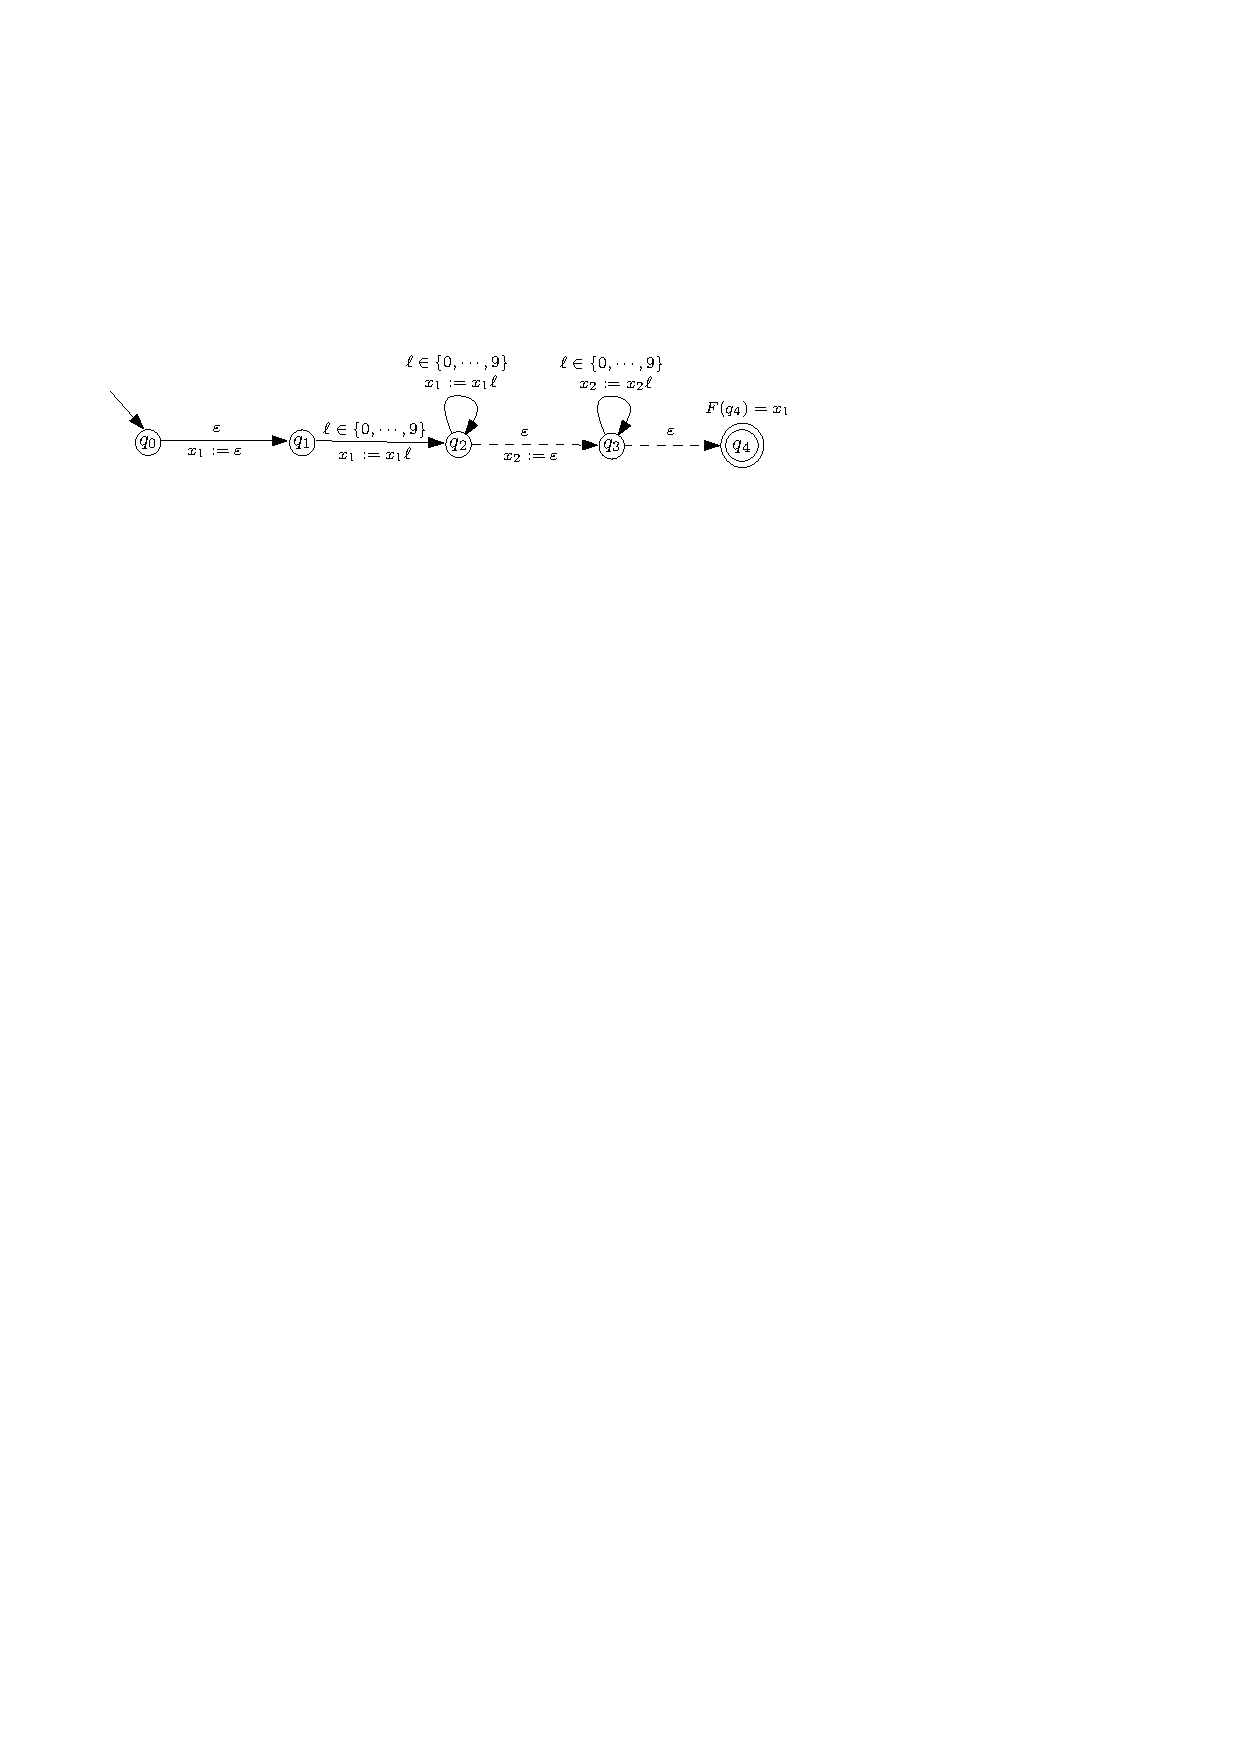
\includegraphics[width=0.8\textwidth]{psst-exmp-decimal.pdf}
\caption{The PSST $\cT$: Extract the matching of the first capturing group in ($\backslash$d+)($\backslash$d*)}
\label{fig-psst-exmp}
%\vspace{-4mm}
\end{figure*}
\end{example}


  
%  $\tmop{Out} (r) =
%  s_{\varepsilon} \circ s_1 \circ s_2 \ldots s_n \circ F (q_n)$ where
%  $s_{\varepsilon}$ is the empty substitution which maps all variables to
%  $\varepsilon$.
  

% Note that in the definition of \NSST, there is no \emph{copyless} restriction.




 
%%%%%%%%%%%%%%%%%%%%%%%%%%%%

%!TEX root = main.tex

\section{Decision procedure for $\strline_{\sf reg}$} \label{sec:decision}

In this section, we shall prove Theorem~\ref{thm-main}, i.e., the decidability of the path feasibility of $\strline_{\sf reg}$. 
%is decidable in XXX. \zhilin{complexity should be added}
%
We first show that semantically equivalent PSSTs can be effectively constructed from the $\extract$ and $\replaceall$ functions. 

\begin{lemma}\label{lem-extract}
A PSST $\cT_{\extract_{i,e}}$ can be constructed for $\extract_{i,e}(x)$ such that $\cR_{\cT_{\extract_{i,e}}} = \{(w, w') \mid w'= \extract_{i,e}(w)\}$.
\end{lemma}

\begin{lemma}\label{lem-replace}
A PSST $\cT_{\replaceall_{\pat, \rep}}$ can be constructed for $\replaceall_{\pat, \rep}(x)$ such that $\cR_{\cT_{\replaceall_{\pat, \rep}}} = \{(w, w') \mid w'= \replaceall_{\pat, \rep}(w)\}$.
\end{lemma}

With Lemma~\ref{lem-extract}-\ref{lem-replace}, the path feasibility of $\strline_{\sf reg}$ is reduced to the path feasibility of string-manipulating programs consisting of  a sequence of the statements of the form $z:=x \concat y$, $y:=\cT(x)$ and $\ASSERT{x \in \cA}$, where $\cT$ is a PSST and $\cA$ is an FA.  The class of programs is denoted by $\strline'_{\sf reg}$. We will  follow %the %backward computation %reasoning approach of 
the general OSTRICH framework \cite{CCH+18,CHL+19} to solve the path feasibility of $\strline'_{\sf reg}$, where the key is to show that the pre-images of regular languages  under PSSTs  are regular and can be computed effectively.

\begin{definition}[Pre-image]
For a string relation $R \subseteq \Sigma^* \times \Sigma^*$ and $L \subseteq \Sigma^*$, we define the \emph{pre-image} of $L$ under $R$ as $R^{-1}(L):=\{w \in \Sigma^* \mid \exists w'.\ w' \in L \mbox{ and } (w, w') \in R\}$. 
\end{definition}
 
\begin{lemma}[Pre-image of \PSST{}]
  \label{lem:psst_preimage}
  Given a \PSST{} $\psst = (Q_T, \Sigma$, $X$, $\delta_T$, $\tau_T$, $E_T$,  $q_{0, T}$, $F_T$) and an \FA{} $\Aut
  = (Q_A, \Sigma, \delta_A, q_{0, A}, F_A)$, we can compute an \FA{} $\cB = (Q_B,
  \Sigma, \delta_B, q_{0, B}, F_B)$ in exponential time  such that $\Lang(\cB) = \cR^{-1}_{\cT}(\Lang(\Aut))$.
\end{lemma}

With Lemma~\ref{lem:psst_preimage}, we  solve the path feasibility of $\strline'_{\sf reg}$ by repeating the following procedure, until no more assignment statements are left. Let $S$ be the current $\strline'_{\sf reg}$ program.
\begin{itemize}
\item If the last assignment statement of $S$ is $y:=\cT(x)$, then let $\ASSERT{y \in \cA_1}$, $\cdots$, $\ASSERT{y \in \cA_n}$ be an enumeration of all the assertion statements for $y$ in $S$. Compute $\cR^{-1}_\cT(\Lang(\cA_1))$ as an FA $\cB_1$, $\cdots$, and $\cR^{-1}_\cT(\Lang(\cA_n))$ as $\cB_n$. Remove  the assignment  $y:=\cT(x)$ and add the assertion statements $\ASSERT{x \in \cB_1}$; $\cdots$; $\ASSERT{x \in \cB_n}$. 
%
\item If the last assignment statement of $S$ is $z:=x \concat y$, then let $\ASSERT{z \in \cA_1}$, $\cdots$, $\ASSERT{z \in \cA_n}$ be an enumeration of all the assertion statements for $z$ in $S$. Compute $\concat^{-1}(\Lang(\cA_1))$, the pre-image of $\concat$ under $\Lang(\cA_1)$, as a collection of FA pairs $(\cB_{1,j}, \cC_{1,j})_{j \in [m_1]}$, $\cdots$, and $\concat^{-1}(\Lang(\cA_n))$ as $(\cB_{n, j}, \cC_{n,j})_{j \in [m_n]}$ (c.f. \cite{CHL+19}). Remove the assignment $z:=x \concat y$, nondeterministically choose the indices $j_1 \in [m_1], \cdots, j_n \in [m_n]$, and add the assertion statements $\ASSERT{x \in \cB_{1,j_1}}; \ASSERT{y \in \cC_{1, j_1}}$; $\cdots$; $\ASSERT{x \in \cB_{n,j_n}}; \ASSERT{y \in \cC_{n, j_n}}$. 
\end{itemize}

\begin{remark}
The aforementioned procedure extends the approach of backward reasoning proposed in \cite{CCH+18,CHL+19}. While standard one-way and two-way transducers were considered in \cite{CCH+18,CHL+19}, we introduce PSST, a new transducer model that covers the $\extract_{i,e}$ and $\replaceall_{\sf pat, rep}$ functions, where priorities are used to model the greedy/non-greedy semantics of $*$/$*?$ and string variables are used to store the matches of capturing groups. 
\end{remark}

It remains to prove Lemma~\ref{lem-extract}-\ref{lem:psst_preimage}, which will be the focus of the next two subsections.
% in Section~\ref{sec-extract-replace-to-psst}-\ref{sec-pre-image}.



%%%%%%%%%%%%%%%%%%%%%%%%%%%%%%%%%%%%%%%%%%%%%%%
\subsection{From $\extract$ and $\replaceall$ to PSST}\label{sec-extract-replace-to-psst}

At first, we can adapt the pNFA construction in \cite{BDM14}, which in turn is a variant of the standard Thompson construction \cite{Thompson68}, and show the following result. 

\begin{proposition}\label{prop-rwre-to-pfa}
For each $\cgexp$ $e$, a PFA $\cA_e$ can be constructed in linear time such that 
\begin{itemize}
\item $\cA_e$ has a unique initial state without incoming transitions and a unique final state without outgoing transitions,
%
\item for subexpression $e'$ of $e$, $\cA_e$ contains an isomorphic copy of $\cA_{e'}$ (i.e. the PFA constructed for $e'$), denoted by ${\sf Sub}_{e'}[\cA_e]$. 
\end{itemize}
\end{proposition}
%Let us use ${\sf Sub}_{e'}[\cA_e]$ to denote the isomorphic copy of $\cA_{e'}$ in $\cA_e$, as mentioned in Proposition~\ref{prop-rwre-to-pfa}.

%
%\begin{theorem}\label{thm-main}
%The path feasibility of $\strline_{\sf reg}$ is decidable.
%\end{theorem}
%




%\subsection{From $\regexp[\sf CG]$ to PFA}
%\label{construction:pnfa}

%\begin{figure*}
%	\centering
%	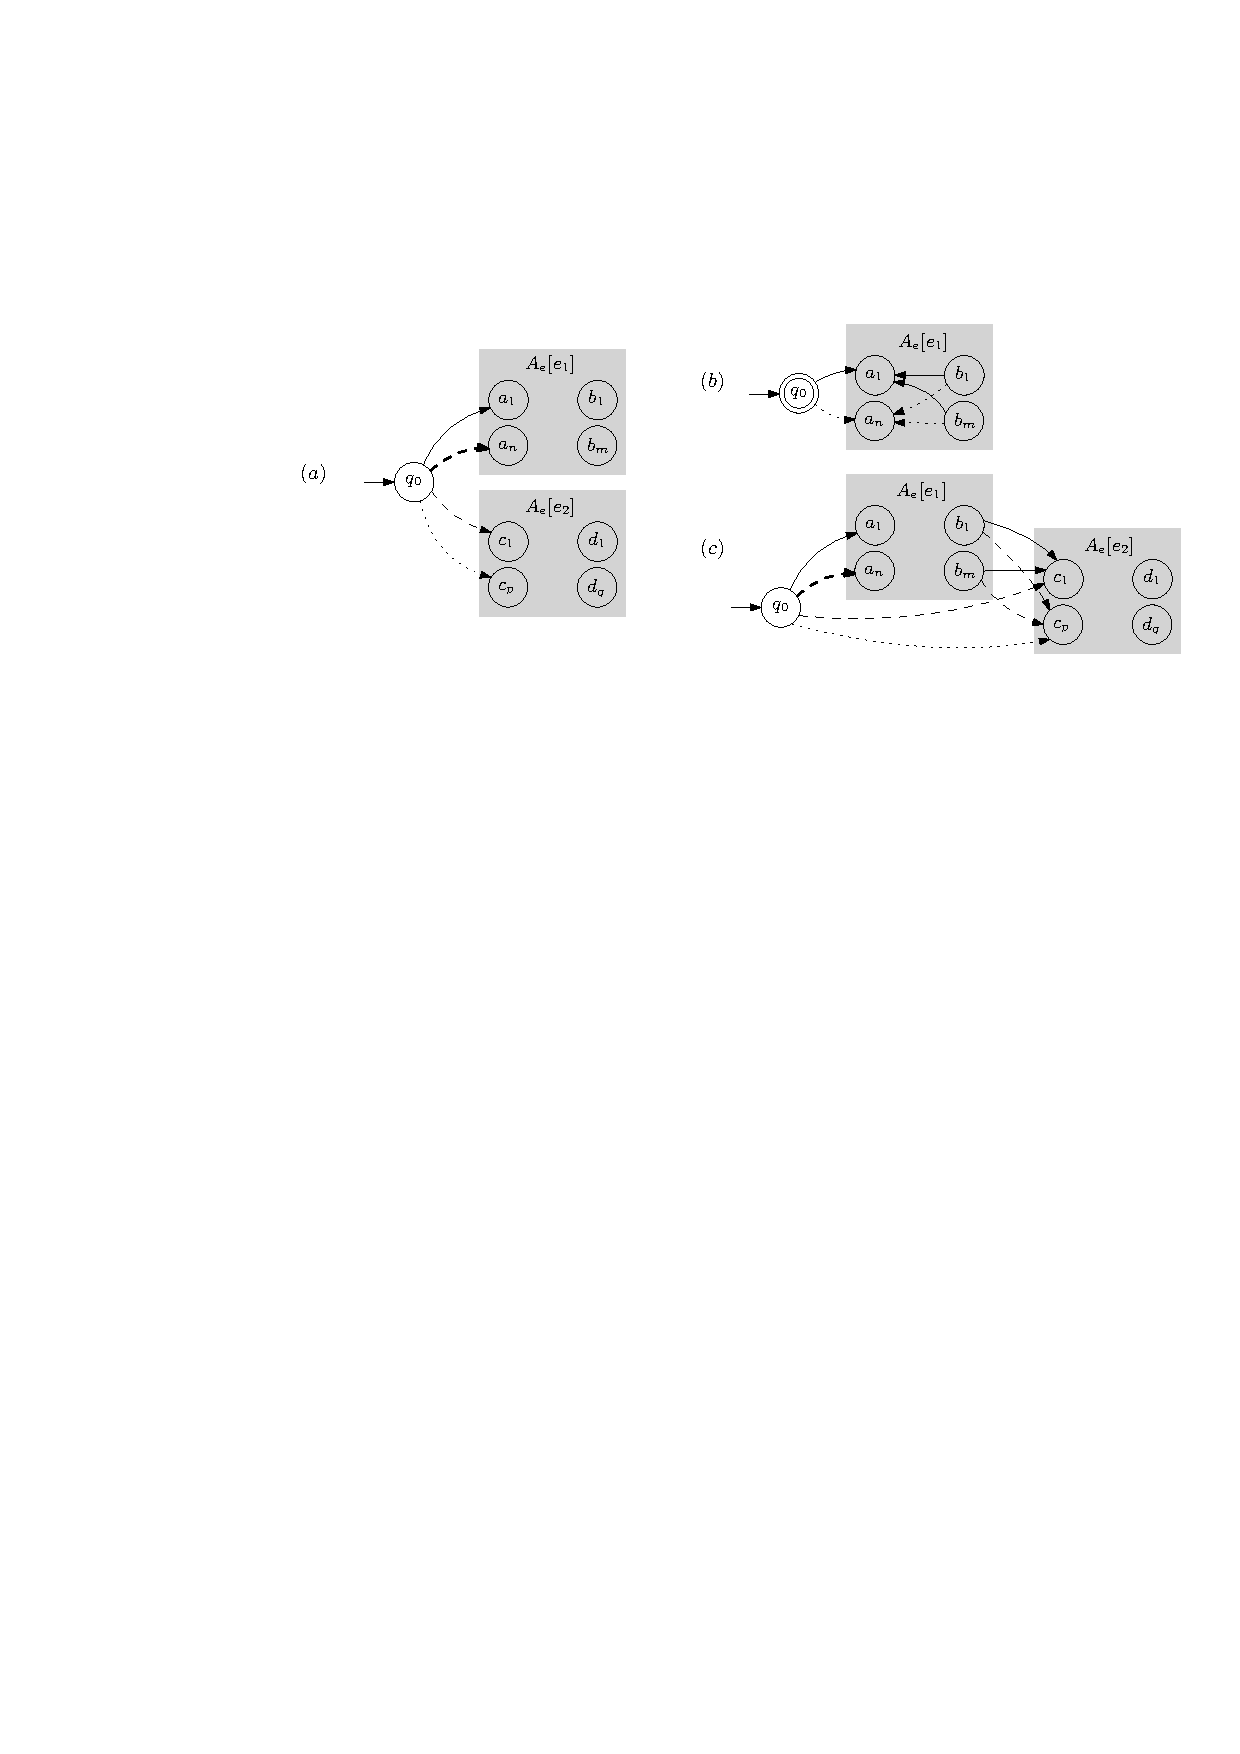
\includegraphics{pglushkov_01}
%	\caption{pNFA $A_e$ for (a) $e=e_1+e_2$ (b) $e=e_1^{\ast}$ and (c) $e=e_1 \concat e_2$ where $\varepsilon \in \Lang(e_1)$ and $\varepsilon \notin \Lang(e_2)$. A transition of lower priority is depicted thiner and more densely dotted. }
%	\label{fig:pglushkov}
%\end{figure*}

%For instance, if $e = (a (ab)^*)^*$ and $e' = a(ab)^*$, then $A_{e}[e']$ is the subgraph of $A_{e}$ comprising the states $\{a_1, a_2, b_3\}$ and the transitions $\{(a_1, a, a_2), (a_2, b, b_3), (b_3, a, a_2)\}$.
 
%Figure.\ref{fig:pglushkov} also illustrates the subgraphs corresponding to direct subexpressions of $e$.


%\begin{definition}
%Let $e \in \regexp[\sf CG]$ and $e'$ be a subexpression of $e$. Then a copy of $\cA_{e'}$ in $\cA_e = (Q, \Sigma, \delta, \tau, q_0, f_0)$ is a PFA $(Q', \Sigma, \delta', \tau', q'_0, f'_0)$ such that  
%\begin{itemize}
%\item $Q' \subseteq Q$, $q'_0, f'_0 \in Q'$, 
%\item $\delta'$ is the restriction of $\delta$ to $Q'$, with the outgoing transitions of $f'_0$ removed, specifically, for every $\sigma \in \Sigma$ and $q \in Q' \setminus \{f'_0\}$, $\delta'(q, \sigma) = \delta(q, \sigma)$, $\tau'(q) = \tau(q)$, $\delta'(f'_0, \sigma) = ()$, and $\tau'(f'_0) = ((); ())$,
%\item $(Q', \Sigma, \delta', \tau', q'_0, f'_0)$ is isomorphic to $\cA_{e'}$.
%\end{itemize}
%\end{definition}

%From the aforementioned recursive construction of $\cA_e$, we know that for each subexpression $e'$ of $e$, a PFA for $e'$, which is isomorphic to $\cA_{e'}$, is also constructed. Let us use ${\sf Sub}_{e'}[\cA_e]$ to denote this PFA for $e'$, which, roughly speaking, is a subgraph of $\cA_e$.


We are ready to prove Lemma~\ref{lem-extract} and Lemma~\ref{lem-replace}.
 
\begin{proof}[Lemma~\ref{lem-extract}]
%\paragraph*{Construction of $\cT_{\extract_{i,e}}$.} 
Let $e'$ be the subexpression corresponding to the $i$-th capturing group of $e$. In particular, if $i=0$, then $e' = e$. 

Suppose $\cA_e = (Q, \Sigma, \delta, \tau, q_0, f_0)$. Moreover, let $\cA^\dag_e = (Q^\dag, \Sigma, \delta^\dag, \tau^\dag, q^\dag_0, f^\dag_0)$ be an isomorphic copy of $\cA_e$, where every state $q$ in $\cA_e$ is replaced by $q^\dag$ in $\cA^\dag_e$. Let us use ${\sf Sub}_{e'}[\cA^\dag_e]$ to denote the isomorphic copy of ${\sf Sub}_{e'}[\cA_e]$ in $\cA^\dag_e$.

Intuitively, $\cT_{\extract_{i,e}}$ contains both $\cA_e$ and $\cA^\dag_e $, and its run comprises two stages: In the first stage, it simulates $\cA_e$. Later on, when it tries to enter a state in ${\sf Sub}_{e'}[\cA_e]$, it enters the second stage and goes to a state in ${\sf Sub}_{e'}[\cA^\dag_e]$, instead of ${\sf Sub}_{e'}[\cA_e]$, and stores the letters into $x$. It outputs $x$ in the state $f^\dag_0$.

Then $\cT_{\extract_{i,e}} = (Q  \cup Q^\dag \cup \{q'_0\}, \Sigma, X, \delta', \tau', E', q'_0, F')$ (see Figure~\ref{fig-psst-extract}), where 
\begin{itemize}
\item $q'_0 \not \in Q \cup Q^\dag$,
%
\item $X = \{x\}$,
%
%\item $\delta'$ is obtained from $\delta$ by adding $x: = x\sigma$ for each transition $(q, \sigma, q')$ in ${\sf Sub}_{e'}[\cA_e]$,  
%
\item $F'(f^\dag_0)= x$ and $F'(p)$ is undefined for all the other states in $p \in Q  \cup Q^\dag \cup \{q'_0\}$,
%
\item $\delta'$ and $\tau'$ are defined as follows,
\begin{itemize}
\item if $q_0$ does not occur in ${\sf Sub}_{e'}[\cA_e]$, then $\tau'(q'_0) = ((q_0), ())$, otherwise, $\tau'(q'_0) = ((q^\dag_0), ())$, 
%
\item for each $q \in Q$ such that $\delta(q) = (q_1, \cdots, q_n)$ and $q$ does not occur in ${\sf Sub}_{e'}[\cA_e]$, we have $\delta'(q) = (q'_1, \cdots, q'_n)$, where for each $i \in [n]$, if $q_i$ occurs in ${\sf Sub}_{e'}[\cA_e]$, then $q'_i = q^\dag_i$, otherwise, $q'_i = q_i$,
%
\item for each $q \in Q$ such that $\tau(q) = (P_1; P_2)$ and $q$ does not occur in ${\sf Sub}_{e'}[\cA_e]$, we have $\tau'(q) = (P'_1; P'_2)$, where $P'_1$ is obtained from $P_1$ by replacing each state $q \in P_1$ occurring in ${\sf Sub}_{e'}[\cA_e]$ with $q^\dag$, similarly for $P'_2$,
%
\item $\delta'$ (resp. $\tau'$) includes all the transitions in $\delta^\dag_e$ (resp. $\tau^\dag_e$),
%
\end{itemize}
%
\item for each transition $(q^\dag_1, \sigma, q^\dag_2)$ in ${\sf Sub}_{e'}[\cA^\dag_e]$ with $\sigma \in \Sigma$, we have $E'((q^\dag_1, \sigma, q^\dag_2))(x) = x \sigma$, and  on all the other transitions, $E'$ does not change the value of $x$.
%
\end{itemize}

\begin{figure}[ht]
\centering
%\rule{\linewidth}{0cm}
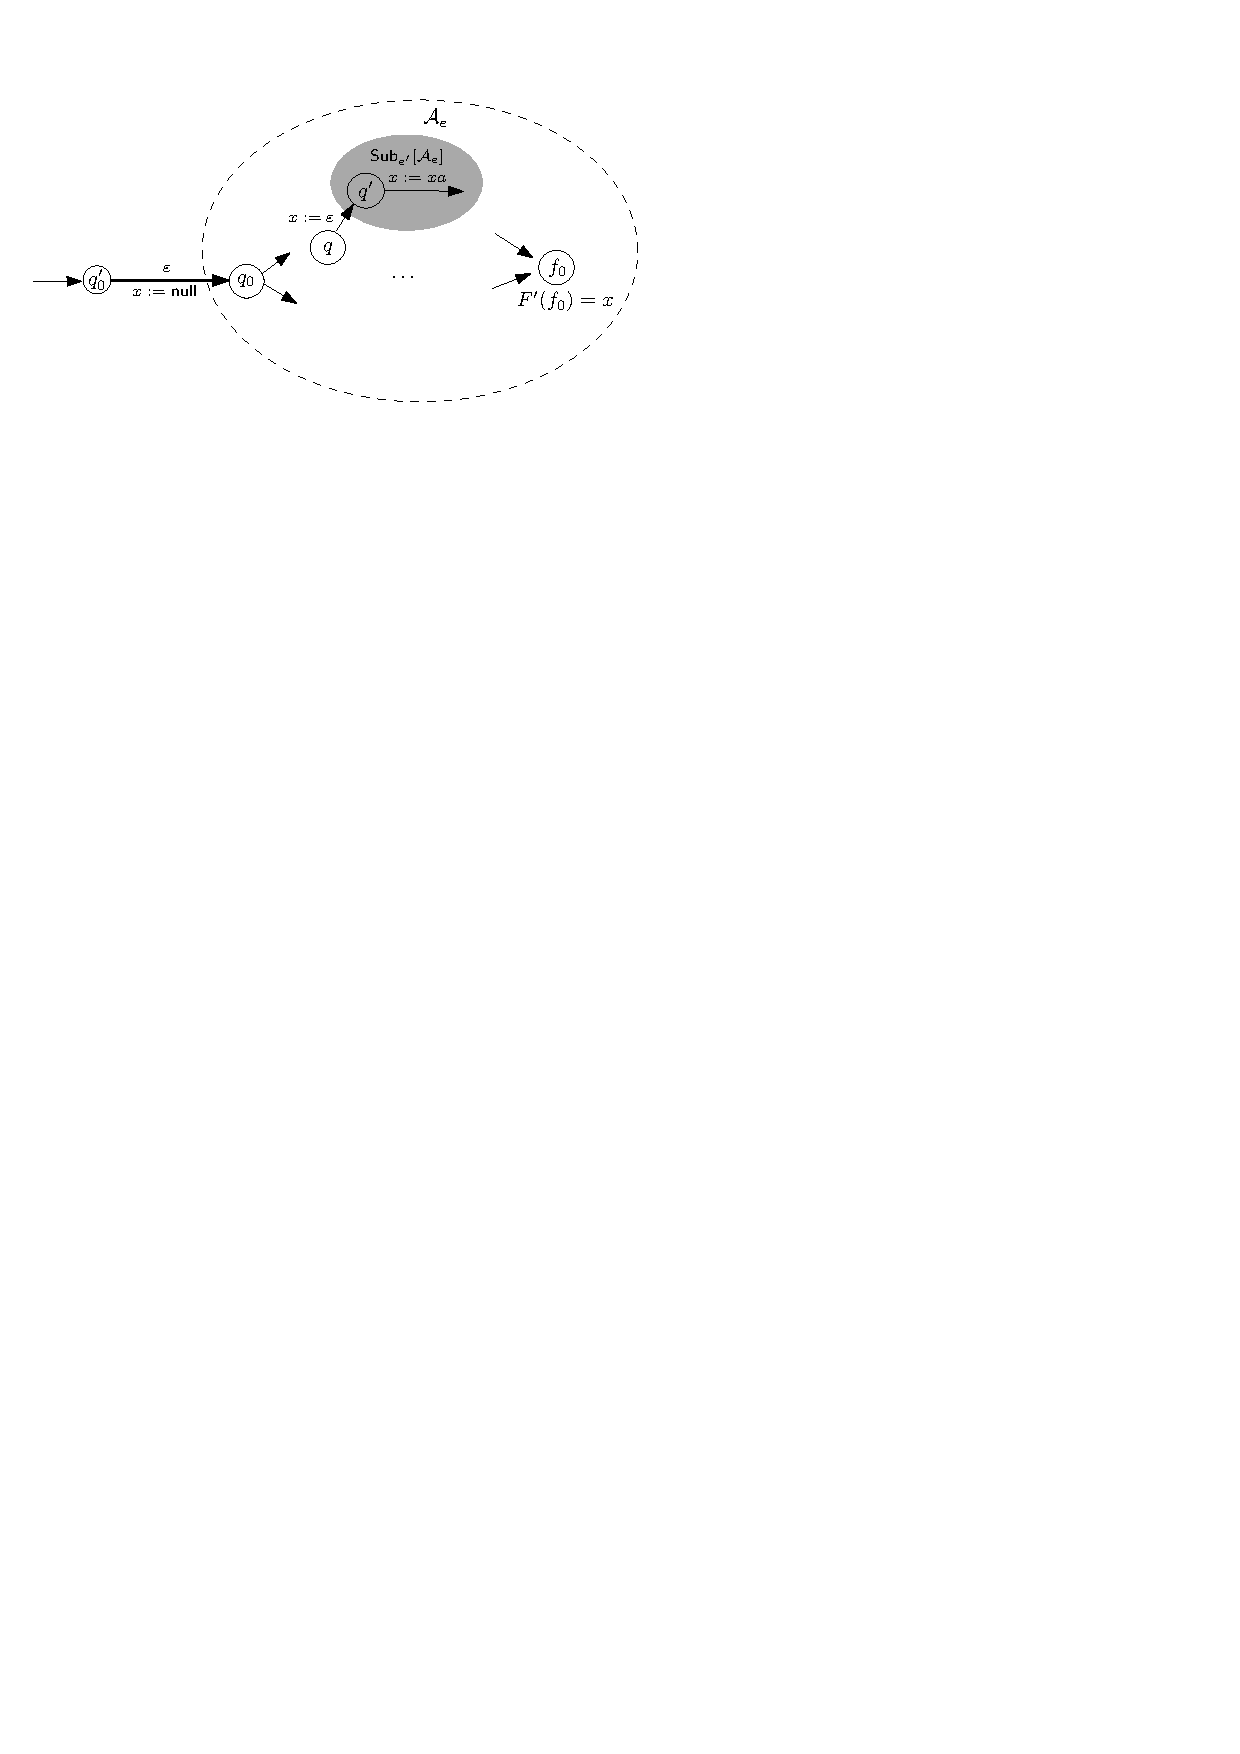
\includegraphics[width = \textwidth]{psst-extract.pdf}
\caption{The PSST for $\extract_{i,e}$}
\label{fig-psst-extract}
\end{figure}
\qed
\end{proof}


\begin{proof}[Lemma~\ref{lem-replace}]
%\paragraph*{Construction of $\cT_{\replaceall_{\pat, \rep}}$.} 
Let $\$i_1, \cdots, \$i_k$ with $i_1 < \cdots < i_k$ be an enumeration of all the references in $\rep$. 
Moreover, for every $j \in [k]$, let $e'_{i_j}$ be the subexpression of $\pat$ corresponding to the $i_j$-th capturing group.

Suppose $\cA_\pat = (Q, \Sigma, \delta, \tau, q_0, f_0)$. Then $\cT_{\replace_{\pat,\rep}}$ is obtained from $\cA_\pat$ by adding a fresh states $q'_0$ such that (see Figure~\ref{fig-psst-replace})
\begin{itemize}
\item $\cT_{\replace_{\pat,\rep}}$ goes from $q'_0$ to $q_0$ via an $\varepsilon$-transition of higher priority than the non-$\varepsilon$-transitions, in order to search the first match of $\pat$ starting from the current position, 
%
\item when $\cT_{\replace_{\pat,\rep}}$ stays at $q'_0$, it keeps appending the current letter to the end of $x_0$, 
%
\item starting from $q_0$, $\cT_{\replace_{\pat,\rep}}$ simulates $\cA_\pat$ and stores the matches of the $\$i_1$-th, $\ldots$, $\$i_k$-th capturing groups of $\pat$ into the string variables $x_1, \cdots, x_k$ respectively,   
%
\item when the first match of $\pat$ is found, $\cT_{\replace_{\pat,\rep}}$ goes from $f_0$ to $q'_0$ via an $\varepsilon$-transition, appends the replacement string, which is $\rep[x_1/\$_{i_1}, \cdots, x_k/\$_{i_k}]$, to the end of $x_0$, and keeps searching for the next match of $\pat$.
\end{itemize}

\begin{figure}[ht]
\centering
%\rule{\linewidth}{0cm}
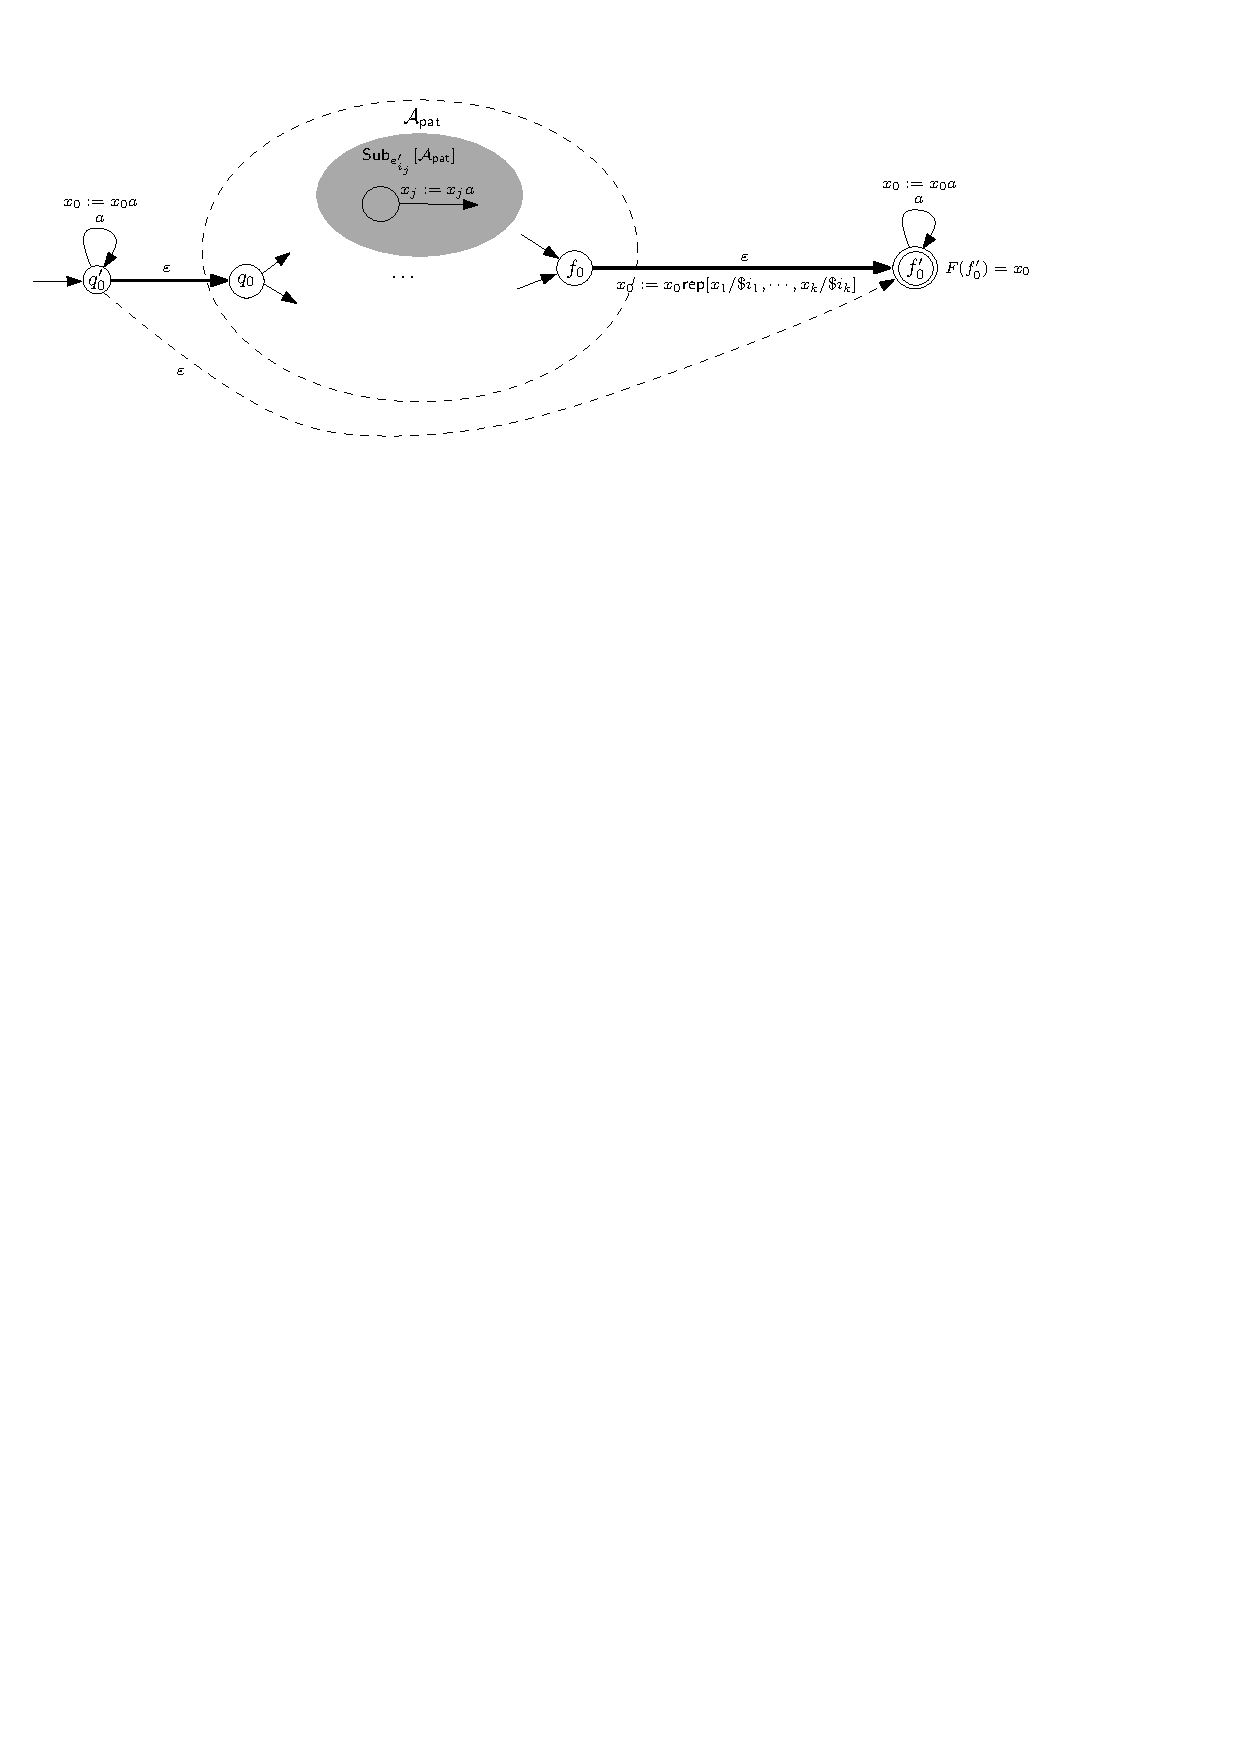
\includegraphics[scale=0.7]{psst-replace.pdf}
\caption{The PSST for $\replace_{\pat,\rep}$}
\label{fig-psst-replace}
\end{figure}

Formally, $\cT_{\replaceall_{\pat, \rep}} =$ $(Q \cup \{q'_0\}$, $\Sigma$, $X$, $\delta'$, $\tau', E, q'_0, F)$ where
\begin{itemize}
\item $q'_0 \not \in Q$,

\item  $X = \{x_0, x_1, \cdots, x_k\}$,
%
\item $F(q'_0) = x_0$, and $F(q')$ is undefined for every $q' \in Q$,
%
\item $\delta'$ and $\tau'$ are obtained from $\delta$ and $\tau$ as follows,
\begin{itemize}
\item $\delta'(q'_0, \sigma) = (q'_0)$ for every $\sigma \in \Sigma$, and $\tau'(q'_0) = ((q_0); ())$,
%
\item for every $q \in Q \setminus \{f_0\}$ and $\sigma \in \Sigma$, $\delta'(q, \sigma) = \delta(q, \sigma)$ and $\tau'(q) = \tau(q)$, 
%
\item $\delta'(f_0, \sigma) = ()$ for every $\sigma \in \Sigma$ and $\tau'(f_0) = ((q'_0); ())$,
\end{itemize}
%
\item $E$ is defined as follows, 
\begin{itemize}
\item for every transition $(q, \sigma, q')$ with $\sigma \in \Sigma^\varepsilon$ in $\cA_\pat$, $E(q, \sigma, q')(x_0) = x_0$,
%
\item for every transition $(q, \sigma, q')$ with $\sigma \in \Sigma^\varepsilon$ and $j \in [k]$,  if $(q, \sigma, q')$ occurs in ${\sf Sub}_{e'_{i_j}}[\cA_\pat]$, then $E(q, \sigma, q')(x_j) = x_j\sigma$, otherwise, $E(q, \sigma, q')(x_j) = x_j$,
%
%\item for all the other transitions $(q, \sigma, q')$ with $\sigma \in \Sigma^\varepsilon$ in $\cA_e$, we have $E(q, \sigma, q')(x) = x$, 
%
\item  for every $\sigma \in \Sigma$ and $j \in [k]$, $E(q'_0, \sigma, q'_0)(x_0) = x_0\sigma$ and $E(q'_0, \sigma, q'_0)$$(x_j) = x_j$, 

\item $E(q'_0, \varepsilon, q_0)(x_j) = x_j$ for every $j \in [k] \cup \{0\}$, 
%
\item $E(f_0, \varepsilon, q'_0)(x_0) = x_0 \rep[x_1/\$i_1,\ldots, x_k/\$i_k]$, and for every $j \in [k]$, we have $E(f_0, \varepsilon, q'_0)(x_j) = \varepsilon$.

\end{itemize}
%
\end{itemize}
\qed
\end{proof}


\subsection{Computing the pre-image of \PSST}\label{sec-pre-image}

In this subsection, we are going to show Lemma~\ref{lem:psst_preimage}, namely, how to compute pre-images of regular languages under PSSTs.

%\tl{another way is to first define B as a PFA, could make the construction a bit modular?}\zhilin{Add a counter example for this natural idea.}
 
Let $\psst = (Q_T, \Sigma$, $X, \delta_T, \tau_T, E_T,  q_{0, T}, F_T)$ be a \PSST{}  and $\Aut
  = (Q_A, \Sigma$, $\delta_A$, $q_{0, A}$, $F_A)$ be an \FA{}. Without loss of generality, we assume that $\Aut$ contains no $\varepsilon$-transitions. 

To illustrate the intuition of the FA construction, let us start with the following natural idea of firstly constructing a PFA $\cB$ for the pre-image: $\cB$ simulates a run of $\psst$ on $w$, and, for each $x \in X$, records an $\Aut$-abstraction of the string stored in $x$, that is, the set of state pairs $(p, q) \in Q_A \times Q_A$ such that starting from $p$, $\Aut$ can reach $q$ after reading the string stored in $x$. Specifically, the states of $\cB$ are of the form $(q, \rho)$ with $q \in Q$ and $\rho \in (\cP(Q_A \times Q_A ))^{X}$. Moreover, the priorities of $\cB$ inherit those of $\Aut$. The PFA $\cB$ is then transformed to an equivalent FA by simply dropping all priorities. We refer to this FA as $\cB'$.

Nevertheless, it turns out that this construction method is flawed: A string $w$ is in $\cR^{-1}_{\cT}(\Lang(\Aut))$ iff the (unique) accepting run of $\cT$ on $w$ produces an output $w'$ that is accepted by $\Aut$. However, a string $w$ is accepted by $\cB'$ iff \emph{there is a run of $\cT$ on $w$, not necessarily of the highest priority}, producing an output $w'$ that is accepted by $\Aut$. The following example illustrates the flaw of the construction above.

\begin{example}
\label{pre-image-count-examp}
Let $\cT_{\tt match_{decimalReg,1}}$ be the PSST in Figure~\ref{fig-psst-exmp} and $\cA$ be the FA corresponding to the regular expression $\{1,\cdots,9\}^*$, specifically, $\cA= (\{p_0\}$, $\{0,\cdots,9\}$, $\delta_A$, $p_0, \{p_0\})$, where $\delta_A = \{(q_0, \ell, q_0) \mid \ell = 1, \cdots, 9\}$.
%  in Figure~\ref{fig-pre-image-count-exmp}, that is, 
%\begin{itemize}
%\item $\cT=(\{q_0, q_1, q_2\}, \{a,b,c\}, \{x_0\}, \delta_T, \tau_T, E_T, q_0, F_T)$, where $\delta_T(q_0, \sigma) = (q_0)$, $\delta_T(q_1, a) = (q_1)$, $\delta_T(q_2, \sigma) = (q_2)$, $\tau_T(q_0) = ((q_1); ())$, $\tau_T(q_1)=((q_0, q_2);())$, and $\tau_T(q_2)= ((); ())$, $E_T(q_0, \sigma, q_0) (x_0) = x_0 \sigma$, $E_T(q_1, \varepsilon, q_0) (x_0) = x_0 c$, $E_T(q_1, \varepsilon, q_2) (x_0) = x_0 c$, $E_T(q_2, \sigma, q_2) (x_0) = x_0 \sigma$, for $\sigma \in\{ a, b\}$. Moreover, $F_T(q_2)= x_0$;
%
%\item $\cA = (\{p_0\}, \{a,b,c\}, \delta_A, p_0, \{p_0\})$, where $\delta_A$ = $\{(p_0, \sigma, p_0)$ $\mid \sigma = b, c\}$.
%\end{itemize}

Let us consider $w = 10$. The accepting run of $\cT_{\tt match_{decimalReg,1}}$ on $w$ is $q_0 \xrightarrow[x_1:=x_11]{1} q_1 \xrightarrow[x_1:=x_10]{0} q_1 \xrightarrow{\varepsilon} q_2 \xrightarrow{\varepsilon} q_3 \xrightarrow{\varepsilon} q_4 \xrightarrow{\varepsilon} q_5 \xrightarrow{\varepsilon} q_6$, producing an output $10 \not \in \Lang(\cA)$. Therefore, $10 \not \in \cR_\cT^{-1}(\Lang(\cA))$. Nevertheless, if we consider the FA $\cB'$ constructed from $\cT$ and $\cA$,  it turns out that $\cB'$ does accept $w$, witnessed by the run $(q_0, \{(p_0,p_0)\}) \xrightarrow{1} (q_1, \{(p_0, p_0)\}) \xrightarrow{\varepsilon} (q_2, \{(p_0, p_0)\}) \xrightarrow{\varepsilon}  (q_3, \{(p_0, p_0)\}) \xrightarrow{\varepsilon}  (q_4, \{(p_0, p_0)\}) \xrightarrow{\varepsilon}  (q_5, \{(p_0, p_0)\}) \xrightarrow{0}  (q_5, \{(p_0, p_0)\}) \xrightarrow{\varepsilon}  (q_6, \{(p_0, p_0)\})$. On the other hand, the run of $\cB'$ corresponding to the accepting run of $\cT$ on $w$, i.e. $(q_0, \{(p_0, p_0)\}) \xrightarrow{1} (q_1, \{(p_0, p_0)\}) \xrightarrow{0} (q_1, \emptyset) \xrightarrow{\varepsilon}  (q_2, \emptyset) \xrightarrow{\varepsilon} (q_3, \emptyset) \xrightarrow{\varepsilon} (q_4, \emptyset) \xrightarrow{\varepsilon} (q_5, \emptyset) \xrightarrow{\varepsilon} (q_6, \emptyset)$, is not accepting, where $\{(p_0,p_0)\}$ and $\emptyset$ are the $\cA$-abstractions of $x_1$.
\end{example}

%%%%%%%%%%%%%%%%%%%%%%%%%%%%%%
%%%%%%%%%%%%%%%%%%%%%%%%%%%%%%
\hide{
\begin{example}
\label{pre-image-count-examp}
Let $\cT$ be the PSST and $\cA$ be the FA in Figure~\ref{fig-pre-image-count-exmp}, that is, 
\begin{itemize}
\item $\cT=(\{q_0, q_1, q_2\}, \{a,b,c\}, \{x_0\}, \delta_T, \tau_T, E_T, q_0, F_T)$, where $\delta_T(q_0, \sigma) = (q_0)$, $\delta_T(q_1, a) = (q_1)$, $\delta_T(q_2, \sigma) = (q_2)$, $\tau_T(q_0) = ((q_1); ())$, $\tau_T(q_1)=((q_0, q_2);())$, and $\tau_T(q_2)= ((); ())$, $E_T(q_0, \sigma, q_0) (x_0) = x_0 \sigma$, $E_T(q_1, \varepsilon, q_0) (x_0) = x_0 c$, $E_T(q_1, \varepsilon, q_2) (x_0) = x_0 c$, $E_T(q_2, \sigma, q_2) (x_0) = x_0 \sigma$, for $\sigma \in\{ a, b\}$. Moreover, $F_T(q_2)= x_0$;
%
\item $\cA = (\{p_0\}, \{a,b,c\}, \delta_A, p_0, \{p_0\})$, where $\delta_A$ = $\{(p_0, \sigma, p_0)$ $\mid \sigma = b, c\}$.
\end{itemize}

Let us consider $w = a$. The accepting run of $\cT$ on $w$ is $q_0 \xrightarrow{\varepsilon} q_1 \xrightarrow[x_0:=x_0c]{\varepsilon} q_0 \xrightarrow[x_0:=x_0a]{a} q_0 \xrightarrow{\varepsilon} q_1 \xrightarrow[x_0:=x_0c]{\varepsilon} q_2$, producing an output $cac \not \in \Lang(\cA)$. Therefore, $a \not \in \cR_\cT^{-1}(\Lang(\cA))$. Nevertheless, if we consider the FA $\cB'$ constructed from $\cT$ and $\cA$,  it turns out that $\cB'$ does accept $w$, witnessed by the run $(q_0, \{(p_0,p_0)\}) \xrightarrow{\varepsilon} (q_1, \{(p_0,p_0)\}) \xrightarrow{a} (q_1, \{(p_0, p_0)\}) \xrightarrow{\varepsilon}  (q_2, \{(p_0, p_0)\})$. On the other hand, the run of $\cB'$ corresponding to the accepting run of $\cT$ on $w$, i.e. $(q_0, \{(p_0,p_0)\}) \xrightarrow{\varepsilon} (q_1, \{(p_0,p_0)\}) \xrightarrow{\varepsilon} (q_0, \{(p_0, p_0)\}) \xrightarrow{a}  (q_0, \emptyset) \xrightarrow{\varepsilon} (q_1, \emptyset) \xrightarrow{\varepsilon} (q_2, \emptyset)$, is not accepting, where $\{(p_0,p_0)\}$ and $\emptyset$ are the $\cA$-abstractions of $x_0$.
\end{example}

\begin{figure}[ht]
\centering
%\rule{\linewidth}{0cm}
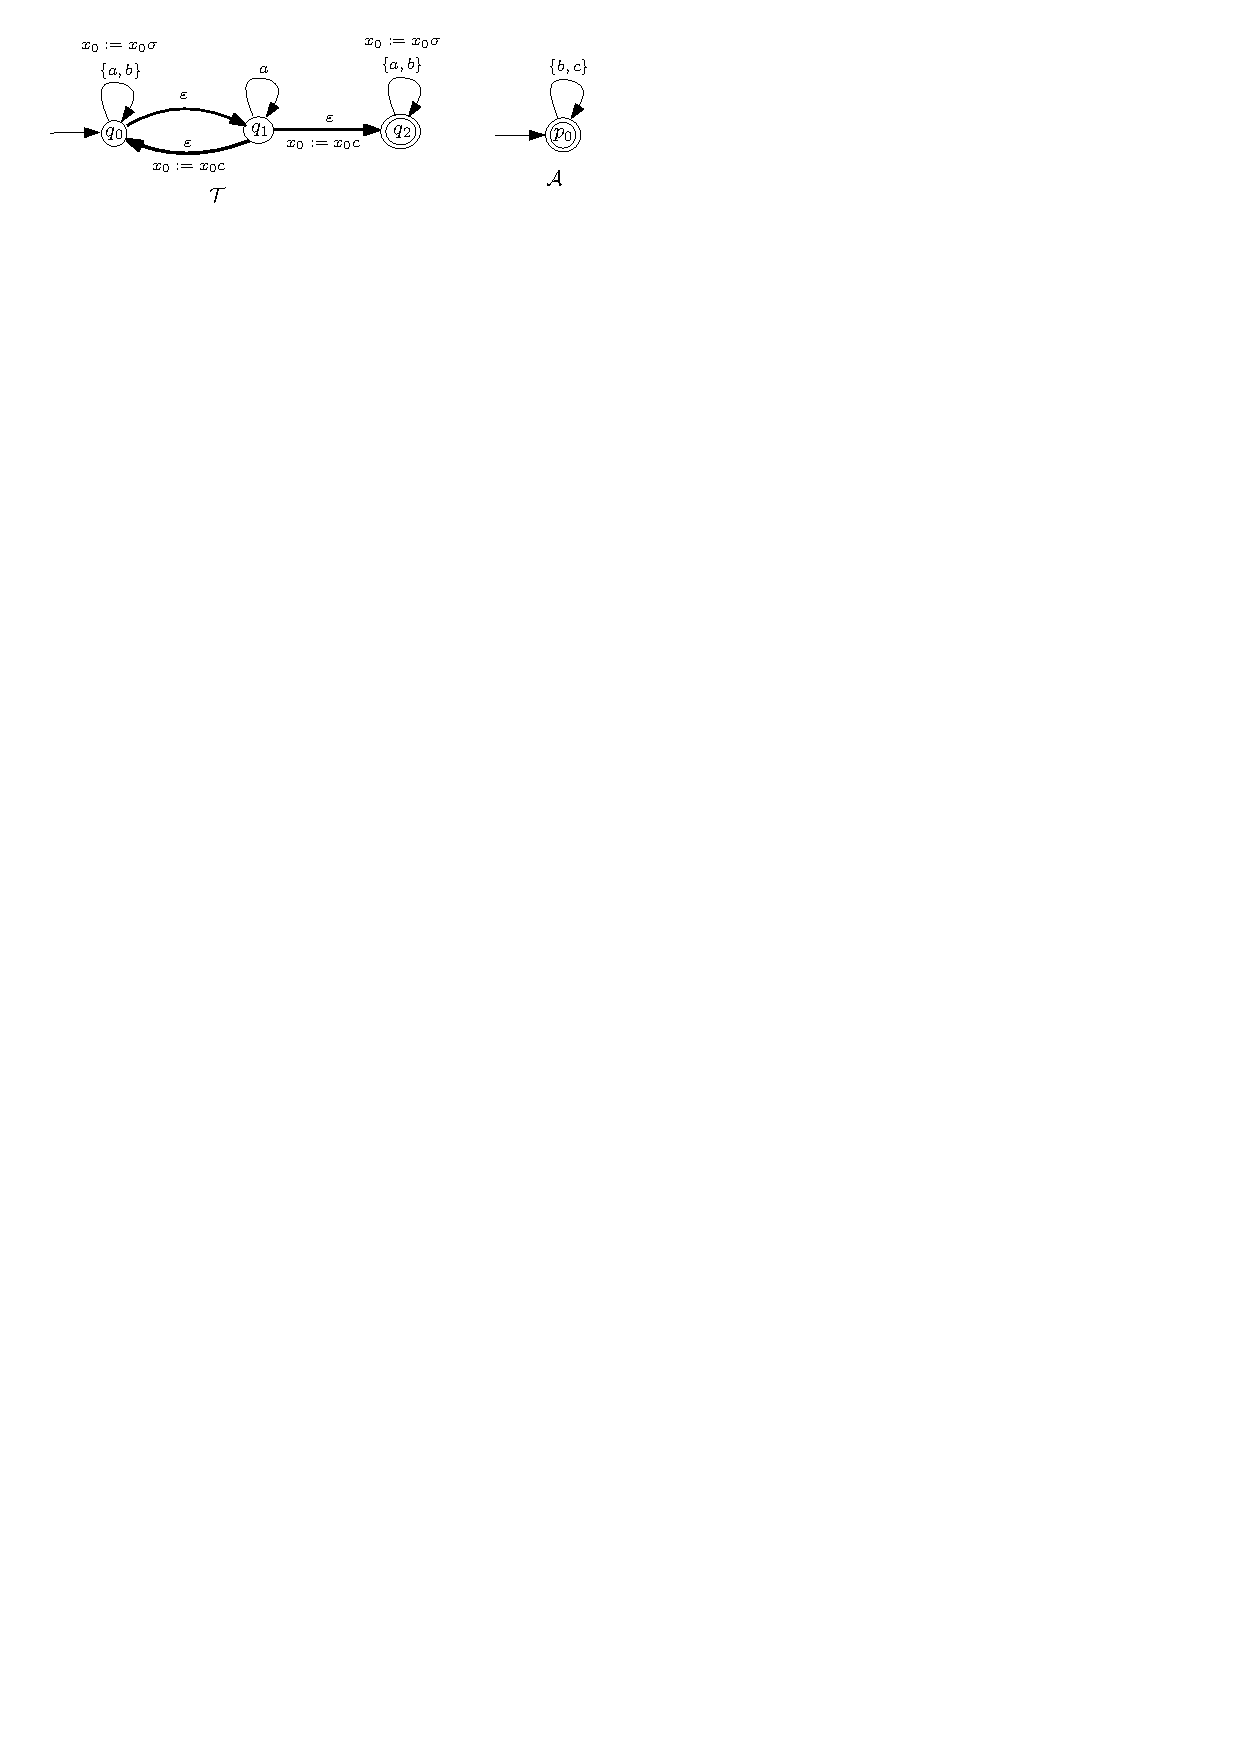
\includegraphics[scale=0.8]{pre-image-counter-example.pdf}
\caption{A counterexample to disprove the flawed pre-image construction method}
\label{fig-pre-image-count-exmp}
\end{figure}
}
%%%%%%%%%%%%%%%%%%%%%%%%%%%%%%%%
%%%%%%%%%%%%%%%%%%%%%%%%%%%%%%%%

\begin{proof}[Lemma~\ref{lem:psst_preimage}]
Let $\psst = (Q_T, \Sigma$, $X, \delta_T, \tau_T, E_T,  q_{0, T}, F_T)$ be a \PSST{} and $\Aut
  = (Q_A, \Sigma, \delta_A, q_{0, A}, F_A)$ be an \FA{}. For convenience, we use $\cE(\tau_T)$ to denote $\{(q, q') \mid q' \in \tau_T(q)\}$.

Our goal is to construct a FA $\cB$ that simulates the run of $\psst$ on $w$, and, for each $x \in X$, records an $\Aut$-abstraction of the string stored in $x$, that is, the set of state pairs $(p, q) \in Q_A \times Q_A$ such that starting from $p$, $\Aut$ can reach $q$ after reading the string stored in $x$. To simulate the runs of $\psst$, it is necessary to record all the states accessible from a run of higher priority to ensure the current run is an accepting run of $\psst$ of highest priority. Moreover, $\cB$ also remembers the set of $\varepsilon$-transitions of $\cT$ after the latest non-$\varepsilon$-transition to ensure that no transition occurs twice in a sequence of $\varepsilon$-transitions of $\cT$.

Specifically, each state of $\cB$ is of the form $(q, \rho, \Lambda, S)$, where $q \in Q_T$, $\rho \in (\cP(Q_A \times Q_A ))^{X}$, $\Lambda \subseteq \cE(\tau_T)$, and $S \subseteq Q_T$. 
For a state $(q, \rho, \Lambda, S)$, our intention for $S$ is that the states in it are those that can be reached in the runs of higher priorities than the current run, by reading the same sequence of letters and applying the $\varepsilon$-transitions as many as possible. Note that when recording in $S$ all the states accessible from a run of higher priority, we do not take the non-repetition of $\varepsilon$-transitions into consideration since if a state is reachable by a sequence of $\varepsilon$-transitions where some $\varepsilon$-transitions are repeated, then there exists also a sequence of non-repeated $\varepsilon$-transitions reaching the state. 
Moreover, when simulating a $\sigma$-transition of $\cT$ (where $\sigma \in \Sigma$) at a state $(q, \rho, \Lambda, S)$, suppose $\delta_T(q, \sigma) = (q_1, \cdots, q_m)$ and $\tau_T(q) = (P_1, P_2)$, then $\cB$ nondeterministically chooses $q_i$ and goes to the state $(q_i, \rho', \emptyset, S')$, where 
\begin{itemize}
\item $\rho'$ is obtained from $\rho$ and $E_T(q, \sigma, q_i)$, 
%
\item $\Lambda$ is reset to $\emptyset$,
% 
\item all the states obtained from $S$ by applying  a $\sigma$ transition should be \emph{saturated by $\varepsilon$-transitions} and put into $S'$, more precisely, all the states reachable from $S$ by first applying a $\sigma$-transition, then a sequence of $\varepsilon$-transitions, should be put into $S'$,
%
\item moreover, all the states obtained from $q_1,\cdots, q_{i-1}$ (which are of higher priorities than $q_i$) by saturating with $\varepsilon$-transitions should be put into $S'$,
%
\item finally, all the states obtained from those in $P'_1 = \{q' \in P_1 \mid (q, q') \not \in \Lambda\}$ (which are of higher priorities than $q_i$) by saturating with non-$\Lambda$ $\varepsilon$-transitions first (i.e. the $\varepsilon$-transitions that do not belong to $\Lambda$), and applying a $\sigma$ transition next, finally saturating with $\varepsilon$-transitions again, should be put into $S'$, (note that according to the semantics of PSST, the $\varepsilon$-transitions in $\Lambda$ should be avoided when defining $P'_1$ and saturating the states in $P'_1$ with $\varepsilon$-transitions). 
\end{itemize}
%For technical reasons, when constructing $\cB$, we assume that this saturation happens when a state is added to $S$ for the first time. Therefore, at a state $(q, \rho, \Lambda, S)$, all the states reachable from the states in $S$ by sequences of $\varepsilon$-transitions in $\cT$ have already been in $S$.

Before the formal construction of $\cB$, we introduce some notations.
\begin{itemize}
\item For $S \subseteq Q_T$, $\delta^{(ip)}_T(S, a) = \{q'_1 \mid \exists q_1 \in S, q'_1 \in \delta_T(q_1, a)\}$.
%
\item For $q \in Q_T$,  if $\tau_T(q) = (P_1, P_2)$, then $\tau^{(ip)}_T(\{q\})=S$ such that $S = P_1 \cup P_2$. 
Moreover, for $S \subseteq Q_T$, we define $\tau^{(ip)}_T(S) = \bigcup \limits_{q \in S} \tau^{(ip)}_T(\{q\})$. We also use $\big(\tau^{(ip)}_T\big)^\ast$ to denote the $\varepsilon$-closure of $\cT$, namely, $\big(\tau^{(ip)}_T\big)^\ast(S) = \bigcup \limits_{n \in \Nat} \big(\tau^{(ip)}_T\big)^{n}(S)$, where $\big(\tau^{(ip)}_T\big)^{0}(S) = S$, and for $n \in \Nat$, $\big(\tau^{(ip)}_T\big)^{n+1}(S) = \tau^{(ip)}_T\big(\big(\tau^{(ip)}_T\big)^{n}(S)\big)$. 
%
\item For $S \subseteq Q_T$ and $\Lambda \subseteq  \cE(\tau_T)$, we use $\big(\tau^{(ip)}_T \backslash \Lambda\big)^\ast(S)$ to denote the set of states reachable from $S$ by sequences of $\varepsilon$-transitions where {\it no} transitions $(q, \varepsilon, q')$ such that $(q, q') \in \Lambda$ are used.
%
%We also use $(\tau^{(ip)}_T)^\ast$ to denote the reflexive transitive closure of $\tau^{(ip)}_T$. \tl{here $(\tau^{(ip)}_T)$ is defined as a function... you mean function composition?}
%\zhilei{I think we can just use the term 'epsilon closure' here?}
%\item For $\sigma \in \Sigma$ and $S \subseteq Q_T$,  we use $\tau^+_T[a, S]$ to denote the set of states that can be obtained from 
% 
\item For $\rho \in (\cP(Q_A \times Q_A ))^{X}$ and $s \in X \rightarrow (X \cup \Sigma)^{\ast}$, we use $s(\rho)$ to denote $\rho'$ that is obtained from $\rho$ as follows: For each $x \in X$, if $s(x) = \varepsilon$, then $\rho'(x) = \{(p, p) \mid p \in Q_A\}$, otherwise, let $s(x) = b_1 \cdots b_\ell$ with $b_i \in \Sigma \cup X$ for each $i \in [\ell]$, then $\rho'(x) = \theta_1 \circ \cdots \circ \theta_\ell$, where $\theta_i = \delta^{(b_i)}_A$ if $b_i \in \Sigma$, and $\theta_i = \rho(b_i)$ otherwise.
\end{itemize}

We are ready to present the formal construction of $\cB =  (Q_B$, $\Sigma$, $\delta_B$, $q_{0, B}, F_B)$. 
\begin{itemize}
\item $Q_B = Q_T \times (\cP(Q_A \times Q_A ))^{X} \times \cP(\cE(\tau_T)) \times \cP(Q_T)$, 
%(Intuitively, the letter $\sigma$ in $(q, \sigma, \rho, S) \in Q_B$ means the next letter to be read at $q$, with $\bot$ represents the end of the input.)

\item $q_{0, B} = (q_{0,T}, \rho_{\varepsilon}, \emptyset, \emptyset)$ where $\rho_{\varepsilon} (x) = \{(q, q) \mid q \in Q\}$ for each $x \in X$,

\item $\delta_{B}$ comprises 
\begin{itemize}
%\item the tuples $(q'_0, \varepsilon, ((q_{0,T},\sigma), \rho_{\varepsilon}, \emptyset))$ where $\sigma \in \Sigma$, $\rho_{\varepsilon} (x) = \{(q, q) \mid q \in Q\}$ for each $x \in X$, 
%
\item the tuples $((q, \rho, \Lambda, S), \sigma, (q_i, \rho', \Lambda', S'))$ such that  
%there exists $s \in \left((X \cup \Sigma\right)^*)^X)$ satisfying
\begin{itemize}
\item $\sigma \in \Sigma$, 
%$\sigma' \in \Sigma \cup \{\bot\}$, 
%
\item $\delta_T (q, \sigma) = (q_1, \ldots, q_i, \ldots, q_m)$, 
%
\item $s = E(q, \sigma, q_i)$, 
%
\item $\rho' = s(\rho)$,
%
\item $\Lambda' = \emptyset$, (Intuitively, $\Lambda$ is reset.)
%
\item let $\tau_T(q) = (P_1, P_2)$, then $S' = \big(\tau^{(ip)}_T\big)^\ast\big(\{ q_1$, $\ldots$, $q_{i - 1} \} \cup \delta^{(ip)}_T\big(S \cup \big(\tau^{(ip)}_T \setminus \Lambda\big)^\ast(P'_1), \sigma\big)\big)$, where $P'_1 = \{q' \in P_1 \mid (q, q') \not \in \Lambda\}$;  
%(Note that according to the semantics of PSSTs, when computing the set of states reachable from $q$ through an $\varepsilon$-transition to some $q' \in P_1$ first and a sequence of $\varepsilon$-transitions starting from $q'$ next, the transitions $(q'', \varepsilon, q''')$ with $(q'', q''') \in \Lambda$ should be excluded. )
%
\end{itemize}
%
\item the tuples $((q, \rho, \Lambda, S), \varepsilon, (q_i, \rho', \Lambda', S'))$ such that 
%there exists $s \in \left((X \cup \Sigma\right)^*)^X$ satisfying
\begin{itemize}
%, $\sigma' \in \Sigma \cup \{\bot\}$, 
%
\item $\tau_T(q) = ((q_1, \ldots, q_i, \ldots, q_m); \cdots)$, 
%
\item $(q, q_i) \not \in \Lambda$,

\item $s = E(q, \varepsilon, q_i)$, 
%
\item $\rho' = s(\rho)$,
%
\item $\Lambda' = \Lambda \cup \{(q, q_i)\}$, 
%
\item $S' =  S \cup \big(\tau^{(ip)}_T \backslash \Lambda \big)^\ast(\{ q_j \mid j \in [i-1], (q, q_j) \not \in \Lambda \})$;
%
%$\rho'(x) = \theta_\ell$ such that $\theta_0 = \{(p,p) \mid p \in Q_A\}$, and for each $i \in [\ell]$, if $b_i \in \Sigma$, then $\theta_i = \{(p, p') \mid (p, p'') \in \theta_{i-1}, (p'', b_i, p') \in \delta_A \mbox{ for some } p''\}$, otherwise, $\theta_i = \theta_{i-1} \cdot \rho(x)$. 
\end{itemize}
%

\item the tuples $((q, \rho, \Lambda, S), \varepsilon, (q_i, \rho', \Lambda', S'))$ such that 
%there exists $s \in \left((X \cup \Sigma\right)^*)^X$ satisfying
\begin{itemize}
%\item $\sigma \in \Sigma$, 
%$\sigma' \in \Sigma \cup \{\bot\}$, 
%
\item $\tau_T (q) = ((q'_1, \ldots, q'_n); (q_1, \ldots, q_i, \ldots, q_m))$, 
%
\item $(q, q_i) \not \in \Lambda$,
%
\item $s = E(q, \varepsilon, q_i)$,
%
\item $\rho' = s(\rho)$,
%
\item $\Lambda' = \Lambda \cup \{(q, q_i)\}$, 
%
\item $S' = S \cup \{q\} \cup \big(\tau^{(ip)}_T \backslash \Lambda \big)^\ast\big(\big\{q'_j \mid j \in [n], (q, q'_j) \not \in \Lambda \big\} \cup \big\{q_j \mid j \in [i-1], (q, q_j) \not \in \Lambda \big\} \big)$. (Note that here we include $q$ into $S'$, since the non-$\varepsilon$-transitions out of $q$ have higher priorities than the transition $(q, \varepsilon, q_i)$.)
%
%$\rho'(x) = \theta_\ell$ such that $\theta_0 = \{(p,p) \mid p \in Q_A\}$, and for each $i \in [\ell]$, if $b_i \in \Sigma$, then $\theta_i = \{(p, p') \mid (p, p'') \in \theta_{i-1}, (p'', b_i, p') \in \delta_A \mbox{ for some } p''\}$, otherwise, $\theta_i = \theta_{i-1} \cdot \rho(x)$. 
\end{itemize}
\end{itemize}
\item
Moreover, $F_B$ is the set of states $(q, \rho, \Lambda, S) \in Q_B$ such that
\begin{enumerate}
  \item $F_T (q)$ is defined,
%
  \item for any $q' \in S$, $F_T (q')$ is not defined,
  %
  \item if $F_T(q) = \varepsilon$, then $q_{0, A}  \in F_A$, otherwise, 
let $F_T(q) = b_1 \cdots b_\ell$ with $b_i \in \Sigma \cup X$ for each $i \in [\ell]$, then $(\theta_1 \circ \cdots \circ \theta_\ell) \cap (\{q_{0,A}\} \times F_A) \neq \emptyset$, where for each $i \in [\ell]$, if $b_i \in \Sigma$, then $\theta_i = \delta^{(b_i)}_A$, otherwise, $\theta_i = \rho(b_i)$.
\end{enumerate}
\end{itemize}
\end{proof}

Note that the above construction  does not utilize the so-called \tmtextit{copyless} property \cite{AC10,AD11},
  thus it works for general, or \textit{copyful} \PSST{} \cite{FR17}.

\begin{example}
Let us continue Example~\ref{pre-image-count-examp}. Suppose $\cT_{\tt match_{decimalReg,1}} = (Q_T, \Sigma$, $X, \delta_T$, $\tau_T, E_T,  q_{0, T}, F_T)$. Then the FA defining $\cR^{-1}_{\cT_{\tt match_{decimalReg,1}}}(\Lang(\Aut))$ constructed by using the aforementioned procedure is illustrated in Figure \ref{fig-psst-preimage-exmp}, where the final states are those boxed states, moreover, the states reachable from $(q_2, \emptyset, \{(q_1,q_2)\}, \{q_1\})$ are omitted because no final states are unreachable from those states, which are therefore redundant. Let us exemplify the construction by considering the state $(q_5, \{(p_0,p_0)\}, \{(q_1,q_2), (q_2,q_3), (q_3,q_4), (q_4, q_5)\}, \{q_1,q_3\})$. For each letter $\ell \in \{0,\cdots, 9\}$, the state $(q_5, \{(p_0,p_0)\}, \emptyset, \{q_1,q_2, q_3, q_4, q_5, q_6\})$ is reached from it, since $\delta(q_1,\ell) = (q_1)$ and $(\tau^{(ip)}_T)^*(\{q_1\}) = \{q_1, q_2, q_3, q_4, q_5, q_6\}$. Note that the state $(q_6, \{(p_0,p_0)\}, \{(q_5,q_6)\}, \{q_1, q_2, q_3, q_4, q_5, q_6\})$ is not a final state since $q_6$ belongs to the last component of the state and $F_T(q_6)$ is defined.
%For efficiency, we minimize the FA after the construction. See Section \ref{sect:impl} for implementation details.
\end{example}


\begin{figure}[ht]
\centering
%\rule{\linewidth}{0cm}
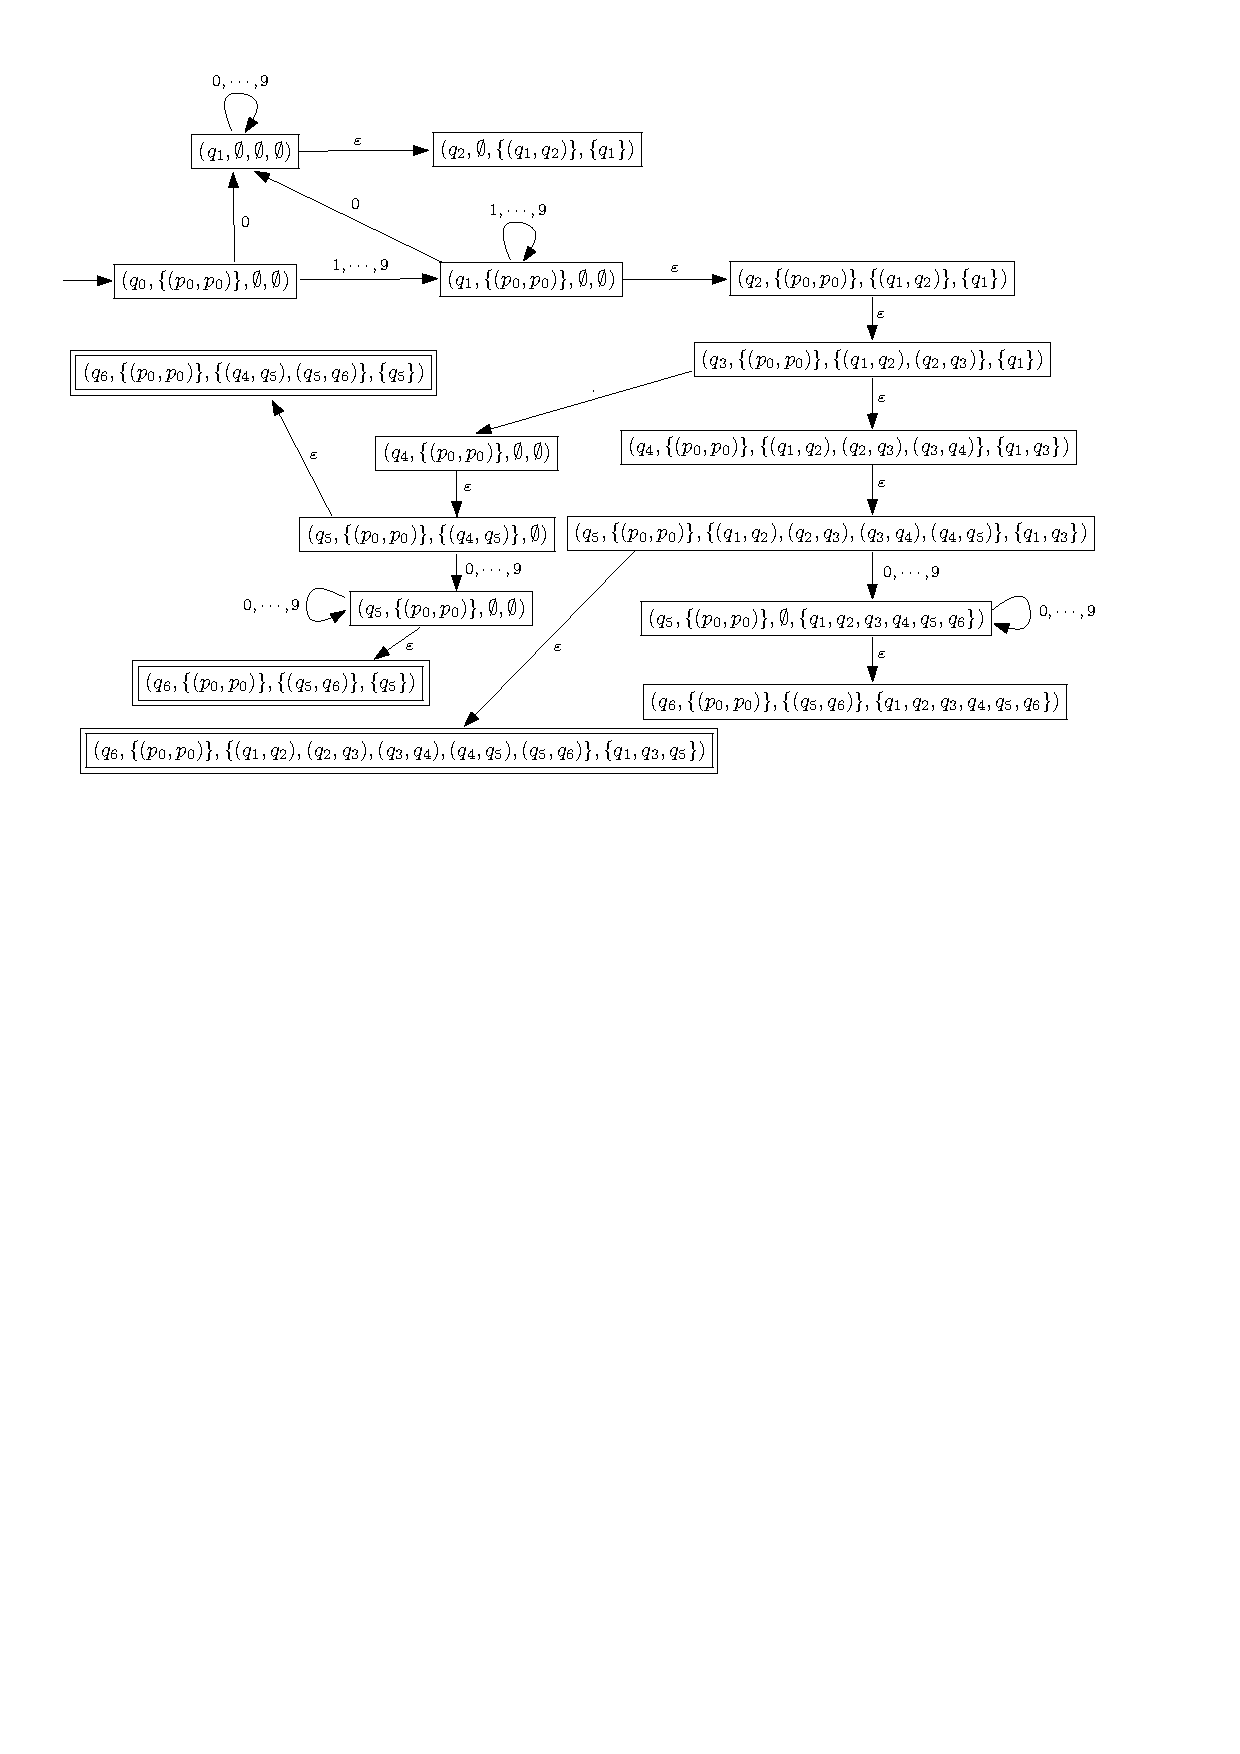
\includegraphics[width = \textwidth]{psst-preimage-example-new.pdf}
\caption{The FA defining $\cR^{-1}_{\cT_{\tt match_{decimalReg,1}}}(\Lang(\Aut))$}
\label{fig-psst-preimage-exmp}
\end{figure}

%%%%%%%%%%%%%%%%%%%%%%%%%%%%%%%%%%%
%%%%%%%%%%%%%%%%%%%%%%%%%%%%%%%%%%%
\hide{
\begin{table}[t]
\centering
\caption{the actual $\cB$ state in Figure 
\label{table:psst-preimage}
\ref{fig-psst-preimage-exmp}}
\begin{tabular}{|c|c|}
    \hline
    Symbol & State of $\cB$\\
    \hline
    $r_0$ & $(q_0, \rho_1, \emptyset, \emptyset)$\\
    \hline
    $r_1$ & $(q_1, \rho_1, \{ (q_0, q_1) \}, \emptyset)$\\
    \hline
    $r_2$ & $(q_2, \rho_1, \{ (q_0, q_1), (q_1, q_2) \}, \{ q_0 \})$\\
    \hline
    $r_3$ & $(q_2, \rho_2, \emptyset, \{ q_0, q_1, q_2 \})$\\
    \hline
    $r_4$ & $(q_2, \rho_1, \emptyset, \{ q_0, q_1, q_2 \})$\\
    \hline
    $r_5$ & $(q_0, \rho_1, \{ (q_0, q_1) (q_1, q_0) \}, \emptyset)$\\
    \hline
    $r_6$ & $(q_0, \rho_2, \emptyset, \emptyset)$\\
    \hline
    $r_7$ & $(q_0, \rho_2, \emptyset, \{ q_0, q_1, q_2 \})$\\
    \hline
    $r_8$ & $(q_1, \rho_2, \{ (q_0, q_1) \}, \{ q_0, q_1, q_2 \})$\\
    \hline
    $r_9$ & $(q_0, \rho_2, \{ (q_0, q_1) (q_1, q_0) \}, \{ q_0, q_1, q_2 \})$\\
    \hline
    $r_{10}$ & $(q_2, \rho_2, \{ (q_0, q_1) (q_1, q_2) \}, \{ q_0, q_1, q_2 \})$\\
    \hline
    $r_{11}$ & $(q_0, \rho_1, \emptyset, \{ q_0, q_1, q_2 \})$\\
    \hline
    $r_{12}$ & $(q_1, \rho_1, \{ (q_0, q_1) \}, \{ q_0, q_1, q_2 \})$\\
    \hline
    $r_{13}$ & $(q_0, \rho_1, \{ (q_0, q_1) (q_1, q_0) \}, \{ q_0, q_1, q_2 \})$\\
    \hline
    $r_{14}$ & $(q_2, \rho_1, \{ (q_0, q_1) (q_1, q_2) \}, \{ q_0, q_1, q_2 \})$\\
    \hline
    $r_{15}$ & $(q_2, \rho_2, \{ (q_0, q_1) (q_1, q_2) \}, \{ q_0 \})$\\
    \hline
    $r_{16}$ & $(q_1, \rho_2, \emptyset, \{ q_0, q_1, q_2 \})$\\
    \hline
    $r_{17}$ & $(q_2, \rho_2, \{ (q_1, q_2) \}, \{ q_0, q_1, q_2 \})$\\
    \hline
    $r_{18}$ & $(q_0, \rho_2, \{ (q_1, q_0) \}, \{ q_0, q_1, q_2 \})$\\
    \hline
    $r_{19}$ & $(q_1, \rho_2, \{ (q_1, q_0) (q_0, q_1) \}, \{ q_0, q_1, q_2 \})$\\
    \hline
    $r_{20}$ & $(q_2, \rho_2, \{ (q_1, q_0) (q_0, q_1) (q_1, q_2) \}, \{ q_0, q_1, q_2 \})$\\
    \hline
    $r_{21}$ & $(q_1, \rho_2, \{ (q_0, q_1) \}, \emptyset)$\\
    \hline
    $r_{22}$ & $(q_0, \rho_2, \{ (q_0, q_1) (q_1, q_0) \}, \emptyset)$\\
    \hline
\end{tabular}
\end{table}
}
%%%%%%%%%%%%%%%%%%%%%%%%%%%%%%%%%%%
%%%%%%%%%%%%%%%%%%%%%%%%%%%%%%%%%%%


\zhilin{stopped here}
\zhilei{changed a little bit}

\subsection{Complexity}

\begin{proposition}[POPL'19]
	The path feasibility problem of the following two fragments is non-elementary: SL with 2FTs, and SL with FTs+replaceAll.
	
	SL[conc, replaceAll, reverse, FFT] is expspace-complete (note that 2FTs in SL are restricted to be one-way and functional)
\end{proposition}

%The same proof strategy can be used for FTs+replaceAll. The 2FTs used in the proof above
%proceed by running completely over the word and producing some output, then silently moving
%back to the beginning of the word. An arbitrary number of passes are made in this way. We
%can simulate this behaviour using FTs and replaceAll.


The main open question is the complexity of the SL fragment with replaceall function and prioritized streaming transducers. Note that PSST can simulate 2FT (adapting Matt's proof?), so we could obtain nonelementary lower bound for SL with PSST.

However, this variant of replaceall is quite different from the replaceall we had before ...

\begin{enumerate}
\item  does  copyless help?
\item how about SL with only this version of replaceall?
\end{enumerate}


%%%%%%%%%%%%%%%%%%%%%%%%%%%%

%!TEX root = main.tex

\section{Implementation and Experiments}
\label{sect:impl}

We have implemented our decision procedure for $\strline_{\sf reg}$ in the SMT
solver \ostrich,\footnote{Name anonymized for doubly-blind review,
and will be provided in the final version.} extending the
open-source solver OSTRICH~\cite{CHL+19}.
%\cite{CHL+19}, %\url{https://github.com/uuverifiers/ostrich}}
%which provides a modular and easy-to-use framework for extending all
%sorts of string operations. 
As shown in Section \ref{sec:decision},
PSSTs satisfy the conditions required by the backward reasoning
approach of OSTRICH, which enables us to integrate our logic with
standard string theory. The resulting extended theory of strings is a
conservative extension of the SMT-LIB theory of Unicode
strings.\footnote{\url{http://smtlib.cs.uiowa.edu/theories-UnicodeStrings.shtml}}

\subsection{Implementation}

Our implementation extends classical regular expressions in SMT-LIB
with indexed {\sf re.capture} and {\sf re.reference} operators, which
denote capturing groups and references to them. We also add {\sf re.*?}
and {\sf re.+?} for lazy Kleene stars.

The three string operators that use these extended real world regular
expressions are {\sf str.replace\_cg}, {\sf str.replace\_cg\_all}, and
{\sf str.extract}. Operators {\sf str.replace\_cg} and {\sf
  str.replace\_cg\_all} are counterparts of the standard {\sf
  str.replace\_re} and {\sf replace\_re\_all} operators, and allow
capturing groups in the match pattern and references in the
replacement pattern. As an example, the following constraint swaps the first name and the last name (see Example~\ref{exmp-name-swap}),
%lower-case characters~$x$ with a sub-sequent upper-case character~$Y$:
%
{\small
\begin{minted}{lisp}
(= w (str.replace_cg_all v (re.++  
 ((_ re.capture 1)(re.+ (re.union (re.range "A" "Z")(re.range "a" "z"))))
 (str.to.re " ") 
 ((_ re.capture 2)(re.+ (re.union (re.range "A" "Z")(re.range "a" "z")))))
 (re.++ (_ re.reference 2) (_ re.reference 1))))
\end{minted}
}
%
The replacement string is written as a regular expression only
containing the operators {\sf re.++}, {\sf str.to\_re}, and {\sf re.reference}. In contrast to the standard operators, using string variables in the 
replacement parameter is not allowed.

The indexed operator {\sf str.extract} implements $\extract_{i, e}$ in
$\strline_{\sf reg}$. For instance,
%
{\small
\begin{minted}{lisp}
  ((_ str.extract 1)
        (re.++ (re.*? re.allchar)
               ((_ re.capture 1) (re.+ (re.range "a" "z")) re.all)) x)
\end{minted}
}
extracts the left-most, longest sub-string consisting of only lower-case
characters from a string~$x$.

Our implementation is able to handle \textit{anchors} as well. Due to space restrictions, we did not introduce them as part of our formalism. Anchors are special symbols that match certain positions of a string without consuming any characters. In most practical programming languages, it is quite common to use \verb!^! and \verb!$! in regular expressions to signify the start and end of a string, respectively. We add \textsf{re.begin-anchor} and \textsf{re.end-anchor} for them.

The implementation revolves around PSSTs. Any of the three string operators mentioned above will be converted into an equivalent PSST (See Appendix~\ref{appendix:sec-extract-replace-to-psst}). {\ostrich} then iterates the dependency graph and repeatedly eliminates them. More specifically, we first use Lemma \ref{lem:psst_preimage} to back-propagate regular constraints on string variables and check satisfiability, and then use forward concrete evaluation to generate a model. We omit the details here due to space restrictions, and refer the readers to the baseline \cite{CHL+19}.

\subsection{Experimental evaluation}

\begin{figure}[tb]
  \scriptsize

  \begin{minipage}{0.49\linewidth}
\begin{minted}{lisp}
(declare-fun x () String)
(define-fun  y () String
   (str.replace_cg_all x <re1> <repl>))
(push 1)
(assert (str.in.re x 
          (re.++ re.all <re1> re.all)))
(assert (str.in.re y 
          (re.++ re.all <re2> re.all)))
(check-sat) (get-model)
(pop 1) (push 1)
(assert (str.in.re x 
          (re.++ re.all <re1> re.all)))
(assert (not (str.in.re y 
          (re.++ re.all <re2> re.all))))
(check-sat) (get-model)
(pop 1) (push 1)
(assert (not (str.in.re x 
          (re.++ re.all <re1> re.all))))
(check-sat) (get-model)
(pop 1)
\end{minted}
  \end{minipage}\hfill
  \raisebox{-25ex}{\rule{0.4pt}{52ex}}\hfill
  \begin{minipage}{0.49\linewidth}
\begin{minted}{js}
function fun(x) {
   if(/<re1>/.test(x)) {
      var y = x.replace(/<re1>/g, <repl>);
      if(/<re2>/.test(y))
        console.log("1");
      else
        console.log("2");
   }
   else
       console.log("3");
}

var S$ = require("S$");
var x = S$.symbol("x", "");
fun(x);
\end{minted}
  \end{minipage}
  
  \caption{Harnesses with replace-all: SMT-LIB for \ostrich,
    and JavaScript for \expose{}.}
  \label{fig:harness}
  
\end{figure}

Our experiments have the purpose of answering the following main questions:

\medskip
\noindent
\textbf{R1:} Are the  RWREs defined in this paper
suitable to encode regular expressions in programming languages,
for instance ECMAScript regular expressions~\cite{ECMAScript11}?
\\
\textbf{R2:} How does \ostrich\ compare to other solvers that can
handle real-world regular expressions, e.g., greedy/lazy
quantifiers and capturing groups?
\\
\textbf{R3:} How does \ostrich\ perform in the context of symbolic execution,
the primary application of string constraint solving?

%

\paragraph{For \textbf{R1}:} We implemented a translator from ECMAScript 11th Edition (ES11 for short) regular
expressions to RWREs, and integrated \ostrich\ into the symbolic
execution tool Aratha~\cite{aratha}. We then ran Aratha+\ostrich\ on
the regression test suite of \expose{}~\cite{DBLP:conf/spin/LoringMK17},
as well as some other JavaScript programs containing match or replace
functions extracted from Github. To verify the soundness of
Aratha+\ostrich, we compared the results with those produced by
\expose{}; we also checked the correctness of models computed by
\ostrich\ by concretely executing the JavaScript program under test on
the generated inputs, to confirm that the concrete execution indeed
follows the targeted path. The results are summarized in Table~\ref{tab:exp-r1};
no inconsistencies were observed in the experiments, showing that the
semantics in this paper are indeed suitable for capturing ES11
semantics.

\begin{table}[t]

	\begin{center}
	\begin{tabular}{|l@{\quad}|*{6}{c}|*{6}{c}|}
	\hline
	   & 
	  \multicolumn{6}{c|}{\textbf{Aratha+\ostrich}} &\multicolumn{6}{c|}{\textbf{\expose{}+Z3}}
	  \\
    & 
	  \multicolumn{6}{c|}{~\# paths covered within 60s~~} &\multicolumn{6}{c@{\quad}|}{~\# paths covered within 60s}
	  \\
	   & ~~0~  & ~1~ &  ~2~ & ~3~ & ~$\geq$4~ & ~\#T.O.~ &
	    ~~0~  & ~1~ &  ~2~ & ~3~ & ~$\geq$4~ & ~\#T.O.~
	  \\\hline
	  \textbf{\expose{}} &  14 & 9 & 9 & 2 & 15 & 0  & 15 & 8 & 9 & 2 & 15 & 1  
	  \\
	  \emph{(49 programs)} & \multicolumn{6}{c|}{Average time: \textbf{6.49}s} & \multicolumn{6}{c@{\quad}|}{Average time: 13.46s}\\
	  & \multicolumn{6}{c|}{Total \#paths covered:126}  & \multicolumn{6}{c@{\quad}|}{Total \#paths covered:122}	  
	  \\\hline
	  \textbf{Match} & 3 & 7 & 12 & 6 & 0 & 0  & 3 & 8 & 12 & 5 & 0 & 6
	  \\
	  \emph{(28 programs)} & \multicolumn{6}{c|}{Average time: \textbf{4.30}s} & \multicolumn{6}{c@{\quad}|}{Average time: 23.66s}\\
	  & \multicolumn{6}{c|}{Total \#paths covered: 49}  & \multicolumn{6}{c@{\quad}|}{Total \#paths covered: 47}	  
	  \\\hline
	  \textbf{Replace} & 12 & 20 & 6 & 0 & 0 & 0  & 12 & 23 & 3 & 0 & 0 & 22
	  \\
	  \emph{(38 programs)} & \multicolumn{6}{c|}{Average time: \textbf{2.71}s} & \multicolumn{6}{c@{\quad}|}{Average time: 41.73s}\\
	  & \multicolumn{6}{c|}{Total \#paths covered: 32}  & \multicolumn{6}{c@{\quad}|}{Total \#paths covered: 29}	  
	  \\\hline
	\end{tabular}
	\end{center}
	\caption{Results of Expose+Z3 and Aratha+{\ostrich} on Javascript programs for \textbf{R1} and \textbf{R3}. Experiments were done on an Intel-Xeon-E5-2690-@2.90GHz machine, running 64-bit Linux and Java 1.8. Runtime was limited to 60s wall-clock time. Average time is
    wall-clock time needed per benchmark, and counts timeouts as 60s. \#T.O. is the number of timeouts. Note that some paths may have already been covered before T.O. }
	\label{tab:exp-r1}
	
\end{table}


\paragraph{For \textbf{R2}:} There are no standard string benchmarks
involving RWREs, and we are not aware of other constraint solvers
supporting capturing groups, neither among the SMT nor the CP
solvers. %(e.g.,
%\cite{DBLP:conf/cpaior/ScottFPS17,DBLP:conf/cp/AmadiniGS20}).
The closest related work is the algorithm implemented in \expose{}, which
applies Z3~\cite{Z3} for solving string constraints, but augments
it with a refinement loop to approximate the RWRE
semantics.\footnote{We considered replacing Z3 with \ostrich\ in
  \expose{} for the experiments. However, \expose{} integrates Z3 using its
  C API, and changing to \ostrich, with native support
  for capture groups, would have required the rewrite of substantial
  parts of \expose{}.}
%
For \textbf{R2}, we compared \ostrich\ with \expose{} on 98,117
RWREs taken from \cite{DMC+19}.

For each of the regular expressions, we created four harnesses: two in
SMT-LIB, as inputs for \ostrich, and two in JavaScript, as inputs for
\expose{}. The two harnesses shown in Fig.~\ref{fig:harness} use one of the
regular expressions from \cite{DMC+19} (\verb!<re1>!) in combination with
the replace-all function to simulate typical string processing;
\verb!<re2>! is the fixed pattern \verb![a-z]+!, and \verb!<repl>! the
replacement string \verb!"$1"!. The three paths of the JavaScript
function~\verb!fun! correspond to the three queries in the SMT-LIB
script, so that a direct comparison can be made between the results of
the SMT-LIB queries and the set of paths covered by \expose{}. The other
two harnesses are similar to the ones in Fig.~\ref{fig:harness}, but
use the match function instead of replace-all, and contain four
queries and four paths, respectively.

\begin{table}[t]

  \begin{center}
  \begin{tabular}{|l@{~~}|*{6}{c}|*{5}{c}@{~~}|}
    \hline
     & 
    \multicolumn{6}{c|}{\textbf{\ostrich}} &
    \multicolumn{5}{c|}{\textbf{\expose{}+Z3}}
    \\
      & \multicolumn{6}{c|}{\# queries solved within 60s}
      & \multicolumn{5}{c|}{\# paths covered within 60s}
    \\
     & ~~0~~ & ~~1~~ & ~~2~~ & ~~3~~ & ~~4~~ & ~~\#Err~~
     & ~~0~~ & ~~1~~ & ~~2~~ & ~~3~~ & ~~4~~
    \\\hline
    \textbf{Match}  & 172 & 92 & 61 & 534 & 96,126 & 1132
    & ~3,333 & 9,274 & 36,916 & 48,594 &
    \\
     \emph{(98,117} & \multicolumn{6}{c|}{Average time: 1.19s}
    &\multicolumn{5}{c|}{Average time: 28.0s}
    \\
    \emph{~~benchm.)} & \multicolumn{6}{c|}{Total \#sat: 249,975, \#unsat: 136,345}
    & \multicolumn{5}{c|}{Total \#paths covered: 228,888}
    \\\hline
    \textbf{Replace} & 445 & 229 & 576 & 95,735 & --- & 1,132
    & ~5,281 & 18,221 & 69,059 & 5,556 & ---
    \\
    \emph{(98,117} & \multicolumn{6}{c|}{Average time: 1.48s}
    & \multicolumn{5}{c|}{Average time: 55.0s}
    \\
    \emph{~~bench.)} & \multicolumn{6}{c|}{Total \#sat: 273,927, \#unsat: 14,659}
    & \multicolumn{5}{c|}{Total \#paths covered: 173,007}
      \\\hline
  \end{tabular}
  \end{center}
  \caption{The number of queries answered by \ostrich, and number of
    paths covered by \expose{}, in the \textbf{R2} experiments. 
    Experiments were done on an AMD Opteron 2220 SE machine, running
    64-bit Linux and Java~1.8.  Runtime per benchmark was limited to
    60s wall-clock time, 2GB memory, and the number of tests
    executed concurrently by \expose\ to 1.  Average time is
    wall-clock time per benchmark, timeouts count as 60s.}
  \label{tab:exp-r2}

\end{table}



The results of this experiment are shown in
Table~\ref{tab:exp-r2}. \ostrich\ is able to answer all four queries
in 96,126 of the match benchmarks (97.9\%), and all three queries in
95,735 of the replace-all benchmarks (97.6\%). The errors in 1,132 cases
are due to back-references in \verb!<re1>!, which are not handled by
\ostrich. \expose{} can on the match problems cover 228,888 paths in
total (91.5\% of the number of sat results of \ostrich), although the
runtime of \expose{} is on average 23x higher than that of
\ostrich. For replace, \expose{} can cover 173,007 paths (63.2\%),
showing that this class of constraints is harder; the runtime of
\expose{} is on average 37x higher than that of \ostrich.  Overall,
even taking into account that \expose{} has to analyze JavaScript
code, as opposed to the SMT-LIB given to \ostrich, the experiments
show that \ostrich\ is a highly competitive solver for RWREs.




\paragraph{For \textbf{R3}:} We compare Aratha+{\ostrich} with
\expose{}+Z3 on the benchmarks from \textbf{R1}. In
Table~\ref{tab:exp-r1}, we can see that Aratha+{\ostrich} can within
60s cover slightly more paths than \expose{}+Z3. Aratha+{\ostrich} can
discover feasible paths more quickly than \expose{}+Z3, however: on
all three families of benchmarks, Aratha+{\ostrich} terminates on
average in less than 10s, and it discovers all paths 
within 35s. \expose{}+Z3 needs full 60s for
29 of the programs (``T.O.'' in the table),
and it finds new paths until the end of the 60s. Since \expose{}+Z3
handles the replace-all operation by unrolling, it is not able to
prove infeasibility of paths involving such operations, and will
therefore not terminate on some programs.
%is faster than \expose{}+Z3 by a factor between 1.7 and 15, while being
%able to cover more paths. The smaller speedup compared to the results
%for \textbf{R2} can be explained by the fact that Aratha should spend time in processing Javascript code, besides using {\ostrich} to solve path constraints.
%SMT-LIB queries
%produced by Aratha are not pure string constraints, but also include
%ADTs, arrays, and bit-vectors. 
Overall, the experiments indicate that {\ostrich} is more
efficient than the CEGAR-augmented symbolic execution for dealing
with RWREs.


%%%%%%%%%%%%%%%%%%%%%%%%%%%%
%\section{Experiments}

%%%%%%%%%%%%%%%%%%%%%%%%%%%%

\bibliographystyle{alpha}
\bibliography{string}

\newpage
%% Appendix
\appendix

%!TEX root = main.tex


\section{Construction of $\CEFA_{\indexof_v}$} \label{appendix:cefa_indexof}

In this section, we show that the function $\indexof_v(\cdot, \cdot)$ can be captured by CEFA. Technically, for any NFA $\NFA$ and constant string $v$, we can construct a CEFA %$\CEFA'$ such that 
accepting $\{(w, (n, \indexof_v(w, n)))\mid w\in \Lang(\NFA) \}$. %$R(\CEFA')=(r_1,r_2)$ and $\Lang(\CEFA')=\{(w, (n, \indexof_v(w, n)))\mid w\in \Lang(\NFA) \}$. 

%The construction is slightly technical and can be found in Appendix, Section~\ref{appendix:cefa_indexof}.
For this purpose, we need a concept of window profiles of  string positions w.r.t. $v$, which are elements of $\{\bot, \top\}^{n-1}$. The window profiles facilitate recognising the first occurrence of $v$ in the input string. 
Intuitively, given a string $u$, the window profile of a position $i$ in $u$ w.r.t. $v$ encodes the matchings of prefixes of $v$ to the suffixes of $u[0,i]$ (see \cite{CCH+18} for the details). For $\pi = \pi_1 \cdots \pi_{n-1} \in \{\bot, \top\}^{n-1}$ and $b \in \Sigma$, we use $\uwp(\vec{\pi}, b)$ to represent the window profile updated from $\pi$ after reading the letter $b$, specifically, $\uwp(\vec{\pi}, b) = \vec{\pi'}$ such that  
\begin{itemize}
\item $\pi'_1 = \top$ iff $b = a_1$, 
%
\item for each $i \in [n-2]$, $\pi'_{i+1} = \top$ iff $\pi_{i} = \top$ and $b = a_{i+1}$. 
\end{itemize}
Let $WP_v$ denote the set of window profiles of string positions w.r.t. $v$. From the result in \cite{CCH+18}, we know that $|WP_v| \le |v|$. 
%Then the set of window profiles of $v$, denoted by $WP_v$, is computed by setting $WP_0 := \{\bot^{n-1}\}$ and iterating the following procedure, until $WP_i = WP_{i+1}$:
%\[WP_{i+1}:=WP_i \cup \{\uwp(\vec{\pi}, b) \mid \vec{\pi} \in WP_i, b \in \Sigma\}.\] 
%Therefore, the aforementioned iteration terminates in at most $|v|$ steps.\\
%
%

Suppose $v = a_1 \cdots a_n$ with $n \ge 2$. 
Then $\indexof_v$ is captured by the CEFA $\CEFA_{\indexof_v}=(Q, \Sigma, R, \delta, I, F)$, such that 
\begin{itemize}
\item $Q = \{q_0, q_1\} \cup WP_v \cup WP_v \times [n]$, 
\item $R=(r_1, r_2)$ (where $r_1,r_2$ represent the input and output positions of $\indexof_v$ respectively), 
\item $I=\{q_0\}$, 
\item $F=\{q_1\}$, and 
\item $\delta$ comprises 
\begin{itemize}
\item the tuples $(q_0, a, q_0, \eta)$ such that $a \in \Sigma$, $\eta(r_1)=1$, and $\eta(r_2) = 1$,
%
\item the tuples $(q_0, a, \vec{\pi}, \eta)$ such that $a \in \Sigma$, $\vec{\pi} = \theta \bot^{n-2}$ where $\theta  = \top$ iff $a = a_1$, $\eta(r_1) = 0$, and $\eta(r_2)= 0$ (recall that the first position of a string is $0$),
% 
\item the tuples  $(\vec{\pi}, a, \uwp(\vec{\pi}, a), \eta)$ such that $\vec{\pi} \in WP_u$, $a \in \Sigma$, $\pi_{n-1} = \bot$ or $a \neq a_{n}$, $\eta(r_1) = 0$, and $\eta(r_2)= 1$,
%
\item the tuples $(\vec{\pi}, a, (\uwp(\vec{\pi}, a), 1), \eta)$ such that $\vec{\pi} \in WP_u$, $a = a_1$, $\pi_{n-1} = \bot$ or $a \neq a_{n}$, $\eta(r_1) = 0$, and $\eta(r_2)= 1$,
%
\item the tuples $((\vec{\pi}, i),  a, (\uwp(\vec{\pi}, a), i+1), \eta)$ such that $\vec{\pi} \in WP_u$, $i \in [n-2]$, $a = a_{i+1}$, $\pi_{n-1} = \bot$ or $a \neq a_{n}$, $\eta(r_1) = 0$, and $\eta(r_2)= 0$,
%
\item the tuples $((\vec{\pi}, n-1),  a, q_1, \eta)$ such that $\vec{\pi} \in WP_u$, $a = a_{n}$, $\eta(r_1) =0$, and $\eta(r_2)= 0$,
%
\item the tuples  $(q_1, a, q_1, \eta)$ such that $a \in \Sigma$, $\eta(r_1) = 0$, and $\eta(r_2)= 0$.
\end{itemize}
\end{itemize}

%%%%%%%%%%%%%%%%%%%%%%%%%%%%%%%%%%%%%%%%%%%%%%%%%%%%%%%%%%%%%%%%%%%%%%%%%%%%%%


\section{Proof of Proposition~\ref{prop:pre-image}}\label{app:pre-image}


\noindent {\bf Proposition~\ref{prop:pre-image}}.
\emph{Let $L$ be a CERL defined by a CEFA $\CEFA = (Q, \Sigma, R, \delta, I, F)$. Then for each string function $f$ ranging over $\concat$, $\replaceall_{e,u}$, $\reverse$, FFTs $\NFT$, and $\substring$, $f^{-1}_R(L)$ is CERR-definable. In addition,
\begin{itemize}
\item a CEFA representation of $\concat^{-1}_R(L)$ can be computed in time $\bigO(|\CEFA|^2)$, 
%
\item a CEFA representation of $\reverse^{-1}_R(L)$ (resp. $\substring^{-1}_R(L)$) can be computed in time $\bigO(|\CEFA|)$,
%
\item a CEFA representation of  $(\Tran(\NFT))^{-1}_R(L)$ can be computed in time polynomial in $|\CEFA|$ and exponential in $|\NFT|$,
%
\item a CEFA representation of  $(\replaceall_{e,u})^{-1}_R(L)$ can be computed in time polynomial in $|\CEFA|$ and exponential in $|e|$ and $|u|$.
\end{itemize}
}

\begin{proof}
	Let $\CEFA=(Q, \Sigma, R, \delta, I, F)$ be a CEFA with $R= (r_1, \cdots, r_k)$. We show how to construct a CEFA representation of $f^{-1}_R(L)$ for each function $f$ in {\slint}.
	
	%%%%%%%%%%%%%%%%%%%%%%%%%%%%%%%%%%%%%%%%%%%%%%%%%%%%%%%%%%%%%%%%%%%%%%%%%%%%%%
	\paragraph*{$\concat^{-1}_R(L)$.}
	%
	A CEFA representation of $\concat^{-1}_R(L)$ is given by $((\CEFA_{I, q}, \NFA_{q, F})_{q \in Q}, \vec{t})$, where 
	\begin{itemize}
		\item $\CEFA_{I, q}=(Q, \Sigma, R^{(1)}, \delta^{(1)}, I, \{q\})$ and  $\CEFA_{q, F}=(Q, \Sigma, R^{(2)}, \delta^{(2)}, \{q\}, F)$ such that 
		\begin{itemize}
			\item $R^{(1)} = (r^{(1)}_1, \cdots, r^{(1)}_k)$, $R^{(2)} = (r^{(2)}_1, \cdots, r^{(2)}_k)$, 
			\item $\delta^{(1)}$ comprises the tuples $(q, a, q', \eta')$ satisfying that there exists $\eta$ such that $(q, a, q', \eta) \in \delta$ and for each $j \in [k]$, and $\eta'(r^{(1)}_j)=\eta(r_j)$,  similarly for $\delta^{(2)}$,
		\end{itemize}
		\item and $\vec{t} = (r^{(1)}_1 + r^{(2)}_1, \cdots, r^{(1)}_k + r^{(2)}_k)$.
	\end{itemize}
	Note that the size of $((\CEFA_{I, q}, \NFA_{q, F})_{q \in Q}, \vec{t})$ is $\bigO(|\CEFA|^2)$.
	%
	%%%%%%%%%%%%%%%%%%%%%%%%%%%%%%%%%%%%%%%%%%%%%%%%%%%%%%%%%%%%%%%%%%%%%%%%%%%%%%
	%
	\paragraph*{$\reverse^{-1}_R(L)$.} 
	%
	A CEFA representation of $\reverse^{-1}_R(L)$ is given by $(\CEFA^{(r)}, \vec{t})$, where 
	\begin{itemize}
		\item $\CEFA^{(r)}=(Q, \Sigma, R^{(1)}, \delta', F, I)$ such that 
		\begin{itemize}
			\item $R^{(1)}=(r^{(1)}_1,\cdots,r^{(1)}_k)$, and 
			\item $\delta'$ comprises the tuples $(q', a, q, \eta')$ satisfying that there exists $\eta$ such that $(q, a, q', \eta) \in \delta$, and $\eta'(r^{(1)}_i) = \eta(r_i)$ for each $i \in [k]$,
		\end{itemize}
		%
		\item and $\vec{t}=(r^{(1)}_1, \cdots, r^{(1)}_k)$. 
	\end{itemize}
	Note that $\Lang(\CEFA^{(r)}) = \{(w^{(r)}, \vec{n}) \mid (w, \vec{n}) \in \Lang(\CEFA)\}$, and the size of $(\CEFA^{(r)}, \vec{t})$ is $\bigO(|\CEFA|)$.
	
	%%%%%%%%%%%%%%%%%%%%%%%%%%%%%%%%%%%%%%%%%%%%%%%%%%%%%%%%%%%%%%%%%%%%%%%%%%%%%%
	\paragraph*{$\substring^{-1}_R(L)$.}
	A CEFA representation of $\substring^{-1}_R(L)$ is given by $(\cB, \vec{t})$, where 
	\begin{itemize}
		\item $\cB = (Q', \Sigma, R', \delta', I', F')$ such that 
		\begin{itemize}
			\item $Q' = Q \times \{p_0, p_1, p_2\}$, (intuitively, $p_0$, $p_1$, and $p_2$ denote that the current position is before the starting position, between the starting position and ending position, and after the ending position respectively)
			%
			\item $R' = \left(r'_{1,1}, r'_{1,2}, r^{(1)}_1,\cdots, r^{(1)}_k \right)$, (intuitively, $r'_{1,1}$ denotes the starting position, and $r'_{1,2}$ denotes the length of the substring)
			%
			\item $I'=I \times \{p_0\}$, $F'=F' \times \{p_2\} \cup (I \cap F) \times \{p_0\}$,
			%
			\item and $\delta'$ comprises 
			\begin{itemize}
				\item the tuples $((q, p_0), a, (q, p_0), \eta')$ such that $q \in I$, $a \in \Sigma$, and $\eta'$ satisfies that $\eta'(r'_{1,1})= 1$, and $\eta'(r'_{1,2}) = 0$, and $\eta'(r^{(1)}_j)=0$ for each $j \in [k]$, 
				%
				\item the tuples $((q, p_0), a, (q', p_1), \eta')$ such that $q \in I$ and there exists $\eta$ satisfying that $(q, a, q', \eta) \in \delta$, moreover, $\eta'(r'_{1,1})=0$ (recall that the positions of strings start at $0$), $\eta'(r'_{1,2}) = 1$, and $\eta'(r^{(1)}_j)=\eta(r_j)$ for each $j \in [k]$,
				%
				\item the tuples $((q, p_0), a, (q', p_2), \eta')$ such that $q \in I$ and there exists $\eta$ satisfying that $(q, a, q', \eta) \in \delta$, moreover, $q' \in F$, and $\eta'(r'_{1,1})=0$ (recall that the positions of strings start at $0$), $\eta'(r'_{1,2}) = 1$, and $\eta'(r^{(1)}_j)=\eta(r_j)$ for each $j \in [k]$,  
				%
				\item the tuples $((q, p_1), a, (q', p_1), \eta')$ such that there exists $\eta$ satisfying that $(q, a, q', \eta) \in \delta$, $\eta'(r'_{1,1}) = 0$, and $\eta'(r'_{1,2}) = 1$, and $\eta'(r^{(1)}_j)=\eta(r_j)$ for each $j \in [k]$,
				%
				\item the tuples $((q, p_1), a, (q', p_2), \eta')$ such that $q' \in F$, and there exists $\eta$ satisfying that $(q, a, q', \eta) \in \delta$, moreover, $\eta'(r'_{1,1}) = 0$, $\eta'(r'_{1,2}) = 1$, and $\eta'(r^{(1)}_j)=\eta(r_j)$ for each $j \in [k]$,
				%
				%\item the tuples $((q, p_1), a, (q, p_2), \eta')$ such that $q \in F$ and $\eta'(r^{(1)}_j)=0$ for each $j \in [k]$, $\eta'(r'_1) = 0$, and $\eta'(r'_2) = 1$,
				%
				\item the tuples $((q, p_2), a, (q, p_2), \eta')$ such that $q \in F$, $\eta'(r'_{1,1}) = 0$, and $\eta'(r'_{1,2}) = 0$, and $\eta'(r^{(1)}_j)=0$ for each $j \in [k]$,
				%
			\end{itemize}
		\end{itemize}
		\item $\vec{t}=(r^{(1)}_1, \cdots, r^{(1)}_k)$.
	\end{itemize}
	Note that the size of $(\cB, \vec{t})$ is $\bigO(|\CEFA|)$.
\zhilin{substring cleaned, the other operations to be cleaned}	
	%%%%%%%%%%%%%%%%%%%%%%%%%%%%%%%%%%%%%%%%%%%%%%%%%%%%%%%%%%%%%%%%%%%%%%%%%%%%%%
	%
	%
	\paragraph*{$(\Tran(\NFT))^{-1}_R(L)$.}
	%
	Suppose $\NFT = (Q', \Sigma, \delta', I', F')$. Then a CEFA representation of $(\Tran(\NFT))^{-1}_R(L)$ is given by 
	$(\cB, \vec{t})$, where 
	\begin{itemize}
		\item $\cB$ simulates the run of $\NFT$ on the input string, meanwhile, it simulates the run of $\CEFA$ on the output string of $\NFT$, formally, $\cB= (Q' \times Q, \Sigma, R^{(1)}, \delta'', I' \times I, F' \times F)$ such that 
		\begin{itemize}
			\item $R^{(1)}  = (r^{(1)}_1, \cdots, r^{(1)}_k)$, and
			\item $\delta''$ comprises the tuples $((q'_1, q_1), a, (q'_2, q_2), \eta')$ satisfying one of the following conditions,
			\begin{itemize}
				\item there exist $u = a_1 \cdots a_n \in \Sigma^+$ and a transition sequence $p_0 \xrightarrow[\delta]{a_1, \eta_1} p_2 \cdots p_{n-1} \xrightarrow[\delta]{a_n, \eta_n} p_{n}$ in $\CEFA$ such that $(q'_1, a, q'_2, u) \in \delta'$, $p_0 = q_1$, $p_{n}= q_2$, and for each $j \in [k]$,  $\eta'(r^{(1)}_j) = \eta_1(r_j) + \cdots + \eta_n(r_j)$,
				%
				\item $(q'_1, a, q'_2, \varepsilon) \in \delta'$, $q_1 = q_2$, and $\eta'(r^{(1)}_j) =0$ for each $j \in [k]$,
			\end{itemize}
		\end{itemize}
		%
		\item $\vec{t}=(r^{(1)}_1, \cdots, r^{(1)}_k)$.
	\end{itemize}
	Note that the number of transitions of $\cB$ can be exponential in the worst case, since it summarises the updates of cost registers of $\CEFA$ on the output strings of the transitions of $\NFT$. More precisely,  let
	\begin{itemize}
		\item $\ell$ be the maximum length of the output strings of transitions of $\NFT$, 
		\item $N$ be the maximum number of transitions between a given pair of states of $\CEFA$, and
		\item  $C$ be the maximum absolute value of the integer constants occurring in $\CEFA$,
	\end{itemize}
	then $|\delta''|$, the cardinality of $\delta''$, is bounded by $|\delta'| \times |Q|^2 \times N^\ell $, and the integer constants occurring in each transition of $\delta''$ are bounded by $\ell C$. Therefore, 
	the size of $(\cB, \vec{t})$ is 
	\[
	\bigO(|\delta'| \times |Q|^2 \times N^\ell \times k \log_2 (\ell C)).
	\] 
	Since $|\delta'|, \ell \le |\NFT|$, $|Q|, N, k \le |\CEFA|$, and $C \le 2^{|\CEFA|}$, we deduce that the size of $(\cB, \vec{t})$ is 
	$
	\bigO( |\NFT| \times  |\CEFA|^2 \times |\CEFA|^{|\NFT|} \times |\CEFA|^2 \log_2(|\NFT|))= |\CEFA|^{\bigO(|\NFT|)} |\NFT| \log_2(|\NFT|).$
	%
	
	%%%%%%%%%%%%%%%%%%%%%%%%%%%%%%%%%%%%%%%%%%%%%%%%%%%%%%%%%%%%%%%%%%%%%%%%%%%%%%
	\paragraph*{$(\replaceall_{e,u})^{-1}_R(L)$.}
	%
	From the result in \cite{CCH+18}, we know that  a NFT $\NFT_{e,u}=(Q', \Sigma, \delta', I', F')$ can be constructed to capture $\replaceall_{e,u}$.  Moreover, 
	\begin{itemize}
		\item $|Q'|$, as well as $|\delta'|$, is $2^{\bigO(|e|)}$,
		\item $\ell$, the maximum length of the output strings of transitions of $\NFT_{e,u}$, is $|u|$.
	\end{itemize}
	Then a CEFA representation of $(\replaceall_{e,u})^{-1}_R(L)$ can be constructed as that of $(\Tran(\NFT_{e,u}))^{-1}_R(L)$.
	Let $N$ denote the maximum number of transitions between a given pair of states of $\CEFA$, and $C$ be the maximum absolute value of the integer constants occurring in $\CEFA$, which is bounded by $2^{|\CEFA|}$. Then the CEFA representation of $(\replaceall_{e,u})^{-1}_R(L)$ is of size 
	\[
	\bigO(|\delta'| \times |Q|^2 \times N^\ell \times k \log_2 (\ell C)) = 2^{\bigO(|e|)} |\CEFA|^2 |\CEFA|^{|u|} |\CEFA|^2 \log_2 |u|=2^{\bigO(|e|)} |\CEFA|^{\bigO(|u|)}.
	\]
	%
	according to the aforementioned discussion for NFTs.
	% 
	%
\end{proof}

%%%%%%%%%%%%%%%%%%%%%%%%%%%%%%%%%%%%%%%%%%%%%%%%%%%%%%%%%%%%%%%%%%%%%%%%%%%%%%%%%%%%%%%%%%%%%%%%%%%%%%%
\section{Proof of Proposition~\ref{prop:la-sat-cefa-inter}}\label{app:sat-cefa}

\noindent{\bf Proposition~\ref{prop:la-sat-cefa-inter}}.
\emph{The {\lasat} problem is $\pspace$-complete.}

\begin{proof}
	The lower bound follows from the {\pspace}-hardness of the intersection problem of NFAs. 
	
	For the upper bound, let $\{ \CEFA_i^{j} \}_{i\in I,j\in J_i}$ be a family of CEFAs  each of which carries a vector of registers $R_i^j$ and  $\phi$ be a quantifier-free LIA formula such that  $ R_i^{j} $ are pairwise disjoint and the variables of $\phi$ are from $R'=\bigcup_{i,j} R_i^j$. 
	%Deciding whether  there are an assignment function $\theta: R' \rightarrow \Int$ and strings $(w_i)_{i \in I}$ such that  $\phi[\theta(R' )/R']$ holds and $(w_i, \theta(R_i^j)) \in \Lang(\CEFA_{i}^j)$ for every $i \in I$ and $j \in J_i$ is $\pspace$-complete. 
	
	At first, we observe that we can focus on \emph{monotonic CEFAs} where the cost registers are monotone in the sense that their values are non-decreasing, in other words, they can only be updated with natural number constants. This observation is justified by the following reduction.
	
	For each register $r \in R^i_j$, introduce two registers $r^+, r^-$. Let $(R^i_j)^{\pm}$ denote the vector of registers by replacing each $r \in R^i_j$ with $(r^+, r^-)$. Intuitively,  for each $r \in R^i_j$, the updates of $r$ in $\CEFA_i^{j} $ are split into the non-negative ones and negative ones, with the former stored in $r^+$ and the latter in $r^-$. Suppose $(R')^{\pm} = \bigcup_{i,j} (R_i^j)^{\pm}$. Then we construct monotonic CEFAs $(\cB_i^{j})_{i \in I, j \in J_i}$ and an LIA formula $\phi^\pm$ such that
	\begin{quote}
		there are an assignment function $\theta: R' \rightarrow \Int$ and strings $(w_i)_{i \in I}$ such that  $\phi[\theta(R' )/R']$ holds and $(w_i, \theta(R_i^j)) \in \Lang(\CEFA_{i}^j)$ for every $i \in I$ and $j \in J_i$ 
		\begin{center} if and only if \end{center}
		there are an assignment function $\theta^\pm: (R')^\pm \rightarrow \Nat$ and strings $(w_i)_{i \in I}$ such that  $\phi^\pm[\theta^\pm((R')^\pm)/(R')^\pm]$ holds and $(w_i, \theta^\pm((R_i^j)^\pm)) \in \Lang(\cB_{i}^j)$ for every $i \in I$ and $j \in J_i$.
	\end{quote}
	For $i \in I$ and $j \in J_i$, the CEFA $\cB_{i}^j$ is obtained from $\CEFA_{i}^j$ by replacing each transition $(q, a, q', \eta)$ in $\CEFA_i^j$ by the transition $(q, a, q', \eta')$ such that for each $r \in R_j^j$, 
	\[
	\eta'(r^+) = \left\{ \begin{array}{l  l}\eta(r), & \mbox{ if } \eta(r) \ge 0 \\ 0 & \mbox{ otherwise} \end{array}\right.,  \eta'(r^-) = \left\{ \begin{array}{l  l} 0, & \mbox{ if } \eta(r) \ge 0 \\ -\eta(r) & \mbox{ otherwise} \end{array}\right..
	\]
	In addition, $\phi^\pm$ is obtained from $\phi$ by replacing each $r \in R'$ with $r^+-r^-$.
	
	\smallskip
	
	It remains to prove the {\lasat} problem for monotonic CEFAs is in {\pspace}, namely,
	\begin{quote}
		given a family of monotonic CEFAs $\{ \CEFA_i^{j} \}_{i\in I,j\in J_i}$ each of which carries a vector of registers $R_i^j$ and a quantifier-free LIA formula $\phi$ such that  $ R_i^{j} $ are pairwise disjoint,  and the variables of $\phi$ are from $R'=\bigcup_{i,j} R_i^j$, deciding whether  there are an assignment function $\theta: R' \rightarrow \Nat$ and strings $(w_i)_{i \in I}$ such that  $\phi[\theta(R' )/R']$ holds and $(w_i, \theta(R_i^j)) \in \Lang(\CEFA_{i}^j)$ for every $i \in I$ and $j \in J_i$ is in {\pspace}.
	\end{quote}
	
	
	We use Proposition 16 in \cite{LB16} to show the result. Proposition 16 in \cite{LB16} is about monotonic counter machines, which can be seen as monotonic CEFAs where each transition contain no alphabet symbol, moreover, $\eta(r) \in \{0,1\}$ for the update function $\eta$ therein.
	
	For each $i\in I$ and $j\in J_i$, let $(\CEFA')_i^j$ be the monotonic counter machine obtained from $\CEFA_i^{j}$ by the following two-step procedure:
	\begin{enumerate}
		\item {[Remove the alphabet symbols]}: Remove alphabet symbols $a$ in each transition $(q, a, q', \eta)$ of $\CEFA_i^{j}$.
		%
		\item {[From binary encoding to unary encoding]}: Replace each transition $(q, q', \eta)$ such that $\ell = \max_{r \in R_i^j} \eta(r) > 1$ with a sequence of transitions $(q, p_1,\eta'_1), \cdots, (p_{\ell-1}, p_\ell, \eta'_\ell)$, where $p_1, \cdots,p_r$ are the freshly introduced states, moreover, $\eta'_j(r) = 1$ if $\eta(r) \ge j$, and $\eta'_j(r)=0$ otherwise. 
	\end{enumerate}
	
	According to Proposition 16 in \cite{LB16}, we have the following, 
	\begin{quote}
		Given a family of monotonic counter machines $\{ \cC_i \}_{i\in I}$ each of which carries a vector of counters $R_i$ and a quantifier-free LIA formula $\phi$ such that $ R_i$ are pairwise disjoint,  and the variables of $\phi$ are from $R'=\bigcup_{i} R_i$. If there are an assignment function $\theta: R' \rightarrow \Nat$ and strings $(w_i)_{i \in I}$ such that  $\phi[\theta(R' )/R']$ holds and $(w_i, \theta(R_i)) \in \Lang(\cC_{i})$ for every $i \in I$, then there are desired $\theta$ and $(w_i)_{i \in I}$ such that for each $i \in I$ and $r \in R_i$, $\theta(r)$ is at most polynomial in the number of states in $\cC_i $, exponential in $|R_i|$, and exponential in $|\phi|$.
	\end{quote}
	For each $i \in I$, let $\cC_i$ be the product of monotonic counter machines $(\CEFA')_i^j$ for $j \in J_i$. 
	From the fact that the number of states of $(\CEFA')_i^j$ is at most the product of the number of transitions of $\CEFA_i^j$ and $B_{\CEFA_i^j}$ (where $B_{\CEFA_i^j}$ denotes the maximum natural number constants $\eta(r)$ in $\CEFA_i^j$), we deduce the following,
	\begin{quote}
		if there are an assignment function $\theta: R' \rightarrow \Nat$ and strings $(w_i)_{i \in I}$ such that  $\phi[\theta(R' )/R']$ holds and $(w_i, \theta(R_i^j)) \in \Lang(\CEFA_i^j)$ for every $i \in I$ and $j \in J_i$, then there are desired $\theta$ and $(w_i)_{i \in I}$ such that for each $r \in \bigcup_{j \in J_i} R^j_i$, $\theta(r)$ is at most polynomial in the product of the number of transitions in $\CEFA_i^j$ and $B_{\CEFA_i^j}$ for $j \in J_i$, exponential in $\left|\bigcup_{j \in J_i} R^j_i \right|$, and exponential in $|\phi|$.
	\end{quote}
	
	Therefore, one can nondeterministically guess the strings $(w_i)_{i \in I}$, and for each $i \in I$ and $j \in J_i$, simulate the runs of CEFAs $\CEFA_i^j$ on $w_i$, in polynomial space, since  the values of all the registers can be assumed to be at most exponential, thus their binary encodings can be stored in polynomial space. From Savitch's theorem \cite{complexity-book}, we conclude that the {\lasat} problem for monotonic CEFAs is in {\pspace}.
\end{proof}

%%%%%%%%%%%%%%%%%%%%%%%%%%%%%%%%%%%%%%%%%%%%%%%%

\section{Example of {\tt urlXssSanitise(url)} for the decision procedure} \label{app:urlexample}

%\begin{example}
	Consider the program $S$ associated with {\tt urlXssSanitise(url)} in Section~\ref{sec:intro}. % Example~\ref{exmp:running}.
	%\[
	%\begin{array}{l}
	%y := \replaceall_{\Sigma \setminus ), \varepsilon}(x); z:= \replaceall_{\Sigma \setminus (, \varepsilon}(x);\\
	%\ASSERT{\length(y) = \length(z)}; \ASSERT{\indexof_{(}(x,0) < \indexof_{)}(x,0)}.
	%\end{array}
	%\] 
	We show how to decide its path feasibility. % of $S$. 
	\begin{description}
		\item[Step I.]   Vacuous since $S$ contains only atomic assertions already. %neither disjunction nor conjunction.
		%
		\item[Step II.] Nondeterministically choose to replace $\indexof_\#(\mathtt{url1}, 0)$ with $-1$ and add $\ASSERT{\mathtt{url1} \in \NFA_{\overline{\Sigma^*\#\Sigma^*}}}$ to $S$.  
		%
		\item[Step III.] Replace $\length(\mathtt{url1})$ with $i'_1$ and add $\ASSERT{\mathtt{url1} \in \CEFA_{\rm len}[i'_1/r_1]}$ to $S$, moreover, replace $\indexof_?(\mathtt{url1}, 0)$ with $i'_3$ and add $\ASSERT{0= i'_2}; \ASSERT{\mathtt{url1} \in \CEFA_{\indexof}[i'_2/r_1, i'_3/r_2]}$ to $S$, where $i'_1, i'_2, i'_3$ are fresh integer variables. Then we get the following program (still denoted by $S$), 
		\[ 
		\begin{array}{l}
		\ASSERT{\mathtt{prothostpath} \in \NFA_\varepsilon}; \ASSERT{\mathtt{querfrag} \in \NFA_\varepsilon}; \mathtt{url1} := \NFT_{\rm trim}(\mathtt{url}); \\
		\ASSERT{\mathtt{qmarkpos} = i'_3}; \ASSERT{\mathtt{sharppos} =-1 }; \ASSERT{\mathtt{qmarkpos} \ge 0}; \\ 
		\mathtt{prothostpath1} := \substring(\mathtt{url1}, 0, \mathtt{qmarkpos});\\
		\mathtt{querfrag1} := \substring(\mathtt{url1, qmarkpos}, i'_1 - \mathtt{qmarkpos});\\
		\mathtt{querfrag2} := \replaceall_{\mathtt{script},\ \varepsilon}(\mathtt{querfrag1});\\
		\mathtt{url2} := \mathtt{prothostpath1} \concat \mathtt{querfrag2}; \ASSERT{\mathtt{querfrag2} \in  \NFA_{\Sigma^*\mathtt{script}\Sigma^*}};  \\
		\ASSERT{\mathtt{url1} \in  \NFA_{\overline{\Sigma^*\#\Sigma^*}}}; \ASSERT{\mathtt{url1} \in \CEFA_{\rm len}[i'_1/r_1]}; \\
		\ASSERT{0= i'_2}; \ASSERT{\mathtt{url1} \in \CEFA_{\indexof}[i'_2/r_1, i'_3/r_2]}.
		\end{array}
		\]
		%
		\item[Step IV.] Since there is no CEFA constraints for $\mathtt{url2}$, removing the last assignment statement of $S$, i.e. $\mathtt{url2} := \mathtt{prothostpath1} \concat \mathtt{querfrag2}$, is easy and in this case we add no statements to $S$. After this, $\mathtt{querfrag2} := \replaceall_{\mathtt{script},\ \varepsilon}(\mathtt{querfrag1})$ becomes the last assignment statement. Suppose $\NFA'=(Q', \Sigma, \delta', I', F')$ is an NFA representing $(\replaceall_{\mathtt{script},\ \varepsilon})^{-1}_\emptyset(\Lang(\NFA_{\Sigma^*\mathtt{script}\Sigma^*}))$, namely, the pre-image of $\Lang(\NFA_{\Sigma^*\mathtt{script}\Sigma^*})$ under $\replaceall_{\mathtt{script},\ \varepsilon}$. Then we remove this assignment statement and add $\ASSERT{\mathtt{querfrag1 \in \NFA'}}$, resulting into the following program
		\[ 
		\begin{array}{l}
		\ASSERT{\mathtt{prothostpath} \in \NFA_\varepsilon}; \ASSERT{\mathtt{querfrag} \in \NFA_\varepsilon}; \mathtt{url1} := \NFT_{\rm trim}(\mathtt{url}); \\
		\ASSERT{\mathtt{qmarkpos} = i'_3}; \ASSERT{\mathtt{sharppos} =-1 }; \ASSERT{\mathtt{qmarkpos} \ge 0}; \\ 
		\mathtt{prothostpath1} := \substring(\mathtt{url1}, 0, \mathtt{qmarkpos});\\
		\mathtt{querfrag1} := \substring(\mathtt{url1, qmarkpos}, i'_1 - \mathtt{qmarkpos});\\
		%    \mathtt{querfrag2} := \replaceall_{\mathtt{script},\ \varepsilon}(\mathtt{querfrag1});\\
		%    \mathtt{url2} := \mathtt{prothostpath1} \concat \mathtt{querfrag2}; 
		\ASSERT{\mathtt{querfrag2} \in  \NFA_{\Sigma^*\mathtt{script}\Sigma^*}};  
		\ASSERT{\mathtt{url1} \in  \NFA_{\overline{\Sigma^*\#\Sigma^*}}}; \\
		\ASSERT{\mathtt{url1} \in \CEFA_{\rm len}[i'_1/r_1]};  \ASSERT{0= i'_2}; \\
		\ASSERT{\mathtt{url1} \in \CEFA_{\indexof}[i'_2/r_1, i'_3/r_2]};  \ASSERT{\mathtt{querfrag1} \in \NFA'}.
		\end{array}
		\]
		
		From Example~\ref{exm:pre-image}, we know that $\substring^{-1}_\emptyset(\Lang(\NFA'))$ can be represented by some CEFA $\cB=(Q'', R'', \delta'', I'', F'')$ with $Q''= Q' \times \{p_0,p_1,p_2\}$ and $R''=(r'_{1,1}, r'_{1,2})$ (where $r'_{1,1}$ and $r'_{1,2}$ are fresh integer variables). Then we remove $\mathtt{querfrag1} := \substring(\mathtt{url1, qmarkpos}, i'_1 - \mathtt{qmarkpos})$, add $\ASSERT{\mathtt{url1} \in \cB};\ASSERT{\mathtt{r'_{1,1}= qmarkpos}}; \ASSERT{r'_{1,2}=i'_1 - \mathtt{qmarkpos}}$, and get the following program
		\[ 
		\begin{array}{l}
		\ASSERT{\mathtt{prothostpath} \in \NFA_\varepsilon}; \ASSERT{\mathtt{querfrag} \in \NFA_\varepsilon}; \mathtt{url1} := \NFT_{\rm trim}(\mathtt{url}); \\
		\ASSERT{\mathtt{qmarkpos} = i'_3}; \ASSERT{\mathtt{sharppos} =-1 }; \ASSERT{\mathtt{qmarkpos} \ge 0}; \\ 
		\mathtt{prothostpath1} := \substring(\mathtt{url1}, 0, \mathtt{qmarkpos});\\
		%   \mathtt{querfrag1} := \substring(\mathtt{url1, qmarkpos}, i'_1 - \mathtt{qmarkpos});\\
		%    \mathtt{querfrag2} := \replaceall_{\mathtt{script},\ \varepsilon}(\mathtt{querfrag1});\\
		%    \mathtt{url2} := \mathtt{prothostpath1} \concat \mathtt{querfrag2}; 
		\ASSERT{\mathtt{querfrag2} \in  \NFA_{\Sigma^*\mathtt{script}\Sigma^*}};  
		\ASSERT{\mathtt{url1} \in  \NFA_{\overline{\Sigma^*\#\Sigma^*}}}; \\
		\ASSERT{\mathtt{url1} \in \CEFA_{\rm len}[i'_1/r_1]};  \ASSERT{0= i'_2}; \\
		\ASSERT{\mathtt{url1} \in \CEFA_{\indexof}[i'_2/r_1, i'_3/r_2]};  \ASSERT{\mathtt{querfrag1} \in \NFA'};\\
		\ASSERT{\mathtt{url1} \in \cB};\ASSERT{\mathtt{r'_{1,1} = qmarkpos} }; \ASSERT{r'_{1,2}=i'_1 - \mathtt{qmarkpos}}.
		\end{array}
		\]
		We can continue the process until the problem contains no assignment statement.
		%
		\item[Step V.]  Straightforward by utilising Proposition~\ref{prop:la-sat-cefa-inter}. 
	\end{description}
%\end{example}








%%%%%%%%%%%%%%%%%%%%%%%%%%%%%%
\section{Algorithms for case splits in the semantics of $\indexof_v$ and $\substring$}\label{app:case-split-semantics}

\begin{algorithm}[htbp]
  \small
  \KwIn{$active$: set of CEFA constraints,  $arith$: arithmetic constraint,
    $\mathit{funApps}$: acyclic set of assignment statements, and $(\mathcal{I}_l)_{l \in [5]}$: subsets of $\indexof_v(x,i)$ string terms}
  \KwResult{$(active, arith, \mathit{funApps})$\newline}
  
\For{each $\indexof_v(x, i) \in \mathcal{I}_1$}
		{
			$arith \leftarrow arith[\indexof_v(x, 0)/\indexof_v(x,i)] \wedge i < 0$\;
		}
		\For{each $\indexof_v(x, i) \in \mathcal{I}_2$}
		{
			$active \leftarrow active \cup \{x \in \NFA_{\overline{\Sigma^* v \Sigma^*}}\}$\;
			$arith \leftarrow arith[-1/\indexof_v(x,i)] \wedge i < 0$\;
		}
		\For{each $\indexof_v(x, i) \in \mathcal{I}_3$}
		{
			$arith \leftarrow arith[-1/\indexof_v(x,i)] \wedge i \ge \length(x)$\;
		}
		\For{each $\indexof_v(x, i) \in \mathcal{I}_4$}
		{
			$arith \leftarrow arith[-1/\indexof_v(x,i)] \wedge i \ge 0 \wedge i < \length(x)$\;
		}
		\For{each $\indexof_v(x, i) \in \mathcal{I}_5$}
		{
			choose fresh variables $y$ and $j$\;
			$active \leftarrow active \cup \{y \in \NFA_{\overline{\Sigma^* v \Sigma^*}}\}$\;
			$arith \leftarrow arith[-1/\indexof_v(x,i)] \wedge i \ge 0 \wedge i < \length(x) \wedge j = \length(x)-i$\;
			 $\mathit{funApps} \leftarrow \mathit{funApps} \cup \{y:=\substring(x, i, j)\}$\;
		}		
\caption{$\mathit{indexofCaseSplit}$ for case splits in the semantics of $\indexof_v$}\label{alg:indexof}
\end{algorithm}

\begin{algorithm}[htbp]
  \small
  \KwIn{$active$: set of CEFA constraints,  $arith$: arithmetic constraint,
    $\mathit{funApps}$: acyclic set of assignment statements, and $(\mathcal{I}_l)_{l \in [5]}$: subsets of $\indexof_v(x,i)$ string terms}
  \KwResult{$(active, arith, \mathit{funApps})$\newline}

  		\For{each $y:=\substring(x, i, j) \in \mathcal{J}_1$}
		{
			 $arith \leftarrow arith \wedge i \ge 0 \wedge i+j \le \length(x)$;
		}
		\For{each $y:=\substring(x, i, j) \in \mathcal{J}_2$}
		{
			 choose a fresh integer variable $i'$\;
			 $arith \leftarrow arith \wedge i \ge 0 \wedge i \le \length(x) \wedge i+j > \length(x) \wedge i' = \length(x)-i$\;
			 $\mathit{funApps} \leftarrow \mathit{funApps}[y:=\substring(x, i, i')/y:=\substring(x, i, j)]$\;
		}
		\For{each $y:=\substring(x, i, j) \in \mathcal{J}_3$}
		{
			 $arith \leftarrow arith \wedge i < 0$\;
			 $active \leftarrow active \cup \{y \in \NFA_\varepsilon\}$\;
			 $\mathit{funApps} \leftarrow \mathit{funApps} \setminus \{y:=\substring(x, i, j)\}$\;		 
		}
\caption{$\mathit{substringCaseSplit}$  for case splits in the semantics of $\substring$}\label{alg:substring}
\end{algorithm}





%%%%%% The proof of Theorem~\ref{thm-la-sat-cefa} is removed%%%%%%%%%%
%%%%%% The proof of Theorem~\ref{thm-la-sat-cefa} is removed%%%%%%%%%%
%%%%%% The proof of Theorem~\ref{thm-la-sat-cefa} is removed%%%%%%%%%%
%%%%%% The proof of Theorem~\ref{thm-la-sat-cefa} is removed%%%%%%%%%%
\hide{
\section{Proof of Theorem~\ref{thm-la-sat-cefa}} \label{appendix:thm-la-sat-cefa}

For a $k$-cost-enriched language $L$, we define 
\[
\prjnum(L) = \left\{(n_1, \cdots, n_k) \in \Int^k \mid \mbox{ there exist } w \in \Sigma^*.\ (w,(n_1,\cdots,n_k)) \in L \right\}.
\]

\begin{lemma}\label{lem-cefa-la}
	Let $\CEFA=(Q, \Sigma, R, \delta, I, F)$ be a CEFA with $R= (r_1, \cdots,  r_k)$. Then an existential LIA formula $\phi_\CEFA(r_1, \cdots, r_k)$ such that $\cM(\phi_\CEFA)= \prjnum(\Lang(\CEFA))$ can be computed in linear time from $\CEFA$.
\end{lemma}

\begin{proof}
	Suppose $\delta = \{\tau_1, \cdots, \tau_l\}$ such that $\tau_j = (q_j, a_j, q'_j, \eta_j)$ and $\eta_j(r_i) =  c_{j,i}$ for every $j \in [l]$ and $i \in [k]$.
	
	From the results on NFAs (Theorem~1 in \cite{SSMH04}), we know that for each pair of states $(q, q') \in I \times F$,  an existential LIA formula $\phi_{q,q'}(m_1, \cdots, m_l)$ can be computed in linear time such that $\cM(\phi_{q,q'})$ is the set of Parikh images of the runs of $\NFA$ starting from $q$ and ending at $q'$, where the variables $m_1, \cdots, m_l$ represent the numbers of occurrences of $\tau_1,\cdots, \tau_l$ respectively in the run. 
	
	Then the desired existential LIA formula $\phi_\NFA$ is constructed as follows,
	\[\phi_\NFA(r_1, \cdots, r_k) ::= \bigvee \limits_{(q,q') \in I \times F} \exists m_1 \cdots \exists m_l.\ \left(\varphi_{q,q'}(m_1, \cdots, m_l) \wedge \bigwedge \limits_{i \in [k]} r_i = \sum \limits_{j \in [l]} c_{j,i} m_j \right).\]
\end{proof}

We are ready to prove Theorem~\ref{thm-la-sat-cefa}.
\begin{proof}[Proof of Theorem~\ref{thm-la-sat-cefa}]
	The NP lower bound follows from the fact that the satisfiability problem of existential LIA formulas is NP-complete \cite{BT76,GS78} (see also \cite{Haase18}).
	
	For the upper bound, suppose that $\phi$ is a quantifier-free LIA formula and $\CEFA_1,\cdots,\CEFA_m$ are CEFAs such that 
	\begin{itemize}
		\item	$\CEFA_i=(Q_i, \Sigma, R_i, \delta_i, I_i, F_i)$  with $R_i = (r_{i, 1}, \cdots, r_{i, k_i})$, for every $i\in [m]$,
		\item $R_i \cap R_j = \emptyset$ for every $1 \le i < j \le m$, and
		\item the free variables of $\phi$ are from $\bigcup_{i\in [m]} R_i$.
	\end{itemize}
	From Lemma~\ref{lem-cefa-la}, for every $i \in [m]$, an existential LIA formula $\phi_{\CEFA_i}(r_{i,1}, \cdots, r_{i, k_i})$ such that $\cM(\phi_{\CEFA_i})= \prjnum(\Lang(\CEFA_i))$ can be computed in linear time from $\CEFA_i$.
	
	Then the satisfiability of $\phi$ w.r.t. $\CEFA_1,\cdots, \CEFA_m$ is reduced to the satisfiability problem of the  following existential LIA formula
	\[
	\phi' \equiv \phi \wedge \bigwedge \limits_{i \in [m]} \phi_{\CEFA_i}(r_{i,1}, \cdots, r_{i, k_i}).
	\]
	Since the size of $\phi'$ is linear in the size of $\phi$ and those of $\CEFA_1,\cdots,\CEFA_m$, and the satisfiability problem of existential LIA formulas is NP-complete, we conclude that the satisfiability of $\phi$ w.r.t.  $\CEFA_1,\cdots,\CEFA_m$ can be decided in nondeterministic polynomial time.
	
	It remains to prove the correctness of the reduction, namely, $\phi$ is satisfiable w.r.t. $\CEFA_1,\cdots, \CEFA_m$ iff $\phi'$ is satisfiable.
	
	\smallskip
	
	\noindent \emph{``Only if'' direction}. Suppose $\phi$ is satisfiable w.r.t. $\CEFA_1,\cdots, \CEFA_m$. Then there are an assignment function $\theta: \bigcup \limits_{i \in [m]} R_i \rightarrow \Int$ and strings $w_1, \cdots, w_m$  
	such that  $\phi[(\theta(R_i)/R_i)_{i \in [m]}]$ is evaluated to $true$ and $(w_i, \theta(R_i)) \in \Lang(\NFA_i)$ for every $i \in [m]$. For every $i \in [m]$, from $\cM(\phi_{\CEFA_i})=\prjnum(\Lang(\CEFA_i))$, we know that $\theta(R_i)$ satisfies $\phi_{\CEFA_i}$, namely, $\phi_{\CEFA_i}[\theta(R_i)/R_i]$ is evaluated to $true$. Therefore, the assignment $\theta$ makes $\phi'$ satisfied.
	
	\smallskip 
	
	\noindent \emph{``If'' direction}. Suppose $\phi'$ is satisfiable. Then there is an assignment $\theta: \bigcup \limits_{i \in [m]} R_i \rightarrow \Int$ such that $\phi[(\theta(R_i)/R_i)_{i \in [m]}]$, $\phi_{\CEFA_1}[\theta(R_1)/R_1]$, $\cdots$, and $\phi_{\CEFA_m}[\theta(R_m)/R_m]$ are all evaluated to $true$. For every $i \in [m]$, from $\cM(\phi_{\CEFA_i})=\prjnum(\Lang(\CEFA_i))$,  we know that there is a string $w_i$ such that $(w_i, \theta(R_i)) \in \Lang(\CEFA_i)$. From Definition~\ref{def-la-sat-cefa}, we conclude that $\phi$ is satisfiable w.r.t. $\CEFA_1,\cdots, \CEFA_m$.
\end{proof}
}
%%%%%% The proof of Theorem~\ref{thm-la-sat-cefa} is removed%%%%%%%%%%
%%%%%% The proof of Theorem~\ref{thm-la-sat-cefa} is removed%%%%%%%%%%



\end{document}
